%%%%%%%%%%%%%%%%%%%%%%%%%%%%%%%%%%%%%%%%%%%%%%%%%%%%%%%%%%%%%%%%%%%%
%%%%%%%%%%%%%%%%%%%%%%%%%%%%%%%%%%%%%%%%%%%%%%%%%%%%%%%%%%%%%%%%%%%%
%%                                                                %%
%% An example for writting your thesis using LaTeX                %%
%% Original version by Luis Costa,  changes by Perttu Puska       %%
%% Support for Swedish added 15092014                             %%
%%                                                                %%
%% This example consists of the files                             %%
%%         thesistemplate.tex (versio 2.01)                       %%
%%         opinnaytepohja.tex (versio 2.01) (for text in Finnish) %%
%%         aaltothesis.cls (versio 2.01)                          %%
%%         kuva1.eps                                              %%
%%         kuva2.eps                                              %%
%%         kuva1.pdf                                              %%
%%         kuva2.pdf                                              %%
%%                                                                %%
%%                                                                %%
%% Typeset either with                                            %%
%% latex:                                                         %%
%%             $ latex opinnaytepohja                             %%
%%             $ latex opinnaytepohja                             %%
%%                                                                %%
%%   Result is the file opinnayte.dvi, which                      %%
%%   is converted to ps format as follows:                        %%
%%                                                                %%
%%             $ dvips opinnaytepohja -o                          %%
%%                                                                %%
%%   and then to pdf as follows:                                  %%
%%                                                                %%
%%             $ ps2pdf opinnaytepohja.ps                         %%
%%                                                                %%
%% Or                                                             %%
%% pdflatex:                                                      %%
%%             $ pdflatex opinnaytepohja                          %%
%%             $ pdflatex opinnaytepohja                          %%
%%                                                                %%
%%   Result is the file opinnaytepohja.pdf                        %%
%%                                                                %%
%% Explanatory comments in this example begin with                %%
%% the characters %%, and changes that the user can make          %%
%% with the character %                                           %%
%%                                                                %%
%%%%%%%%%%%%%%%%%%%%%%%%%%%%%%%%%%%%%%%%%%%%%%%%%%%%%%%%%%%%%%%%%%%%
%%%%%%%%%%%%%%%%%%%%%%%%%%%%%%%%%%%%%%%%%%%%%%%%%%%%%%%%%%%%%%%%%%%%

%% Uncomment one of these:
%% the 1st when using pdflatex, which directly typesets your document in
%% pdf (use jpg or pdf Figures), or
%% the 2nd when producing a ps file (use eps Figures, don't use ps Figures!).
\documentclass[english,12pt,a4paper,pdftex,elec,utf8]{aaltothesis}
%\documentclass[english,12pt,a4paper,dvips]{aaltothesis}

%% To the \documentclass above
%% specify your school: arts, biz, chem, elec, eng, sci
%% specify the character encoding scheme used by your editor: utf8, latin1

%% Use one of these if you write in Finnish (see the Finnish template):
%%
%\documentclass[finnish,12pt,a4paper,pdftex,elec,utf8]{aaltothesis}
%\documentclass[finnish,12pt,a4paper,dvips]{aaltothesis}
\usepackage[super]{nth}
\usepackage{graphicx}
\graphicspath{ {images/} }
\usepackage{listings}
\usepackage{minted}
\usepackage{float}
\usepackage{svg}
\usepackage{pdfpages}

\usepackage{booktabs}
\usepackage{multirow}

%% Use this if you write hard core mathematics, these are usually needed
\usepackage{amsfonts,amssymb,amsbsy}


%% Use the macros in this package to change how the hyperref package below 
%% typesets its hypertext -- hyperlink colour, font, etc. See the package
%% documentation. It also defines the \url macro, so use the package when 
%% not using the hyperref package.
%%
%\usepackage{url}

%% Use this if you want to get links and nice output. Works well with pdflatex.
\usepackage{hyperref}
\hypersetup{pdfpagemode=UseNone, pdfstartview=FitH,
  colorlinks=true,urlcolor=red,linkcolor=blue,citecolor=black,
  pdftitle={Default Title, Modify},pdfauthor={Your Name},
  pdfkeywords={Modify keywords}}


%% All that is printed on paper starts here
\begin{document}

%% Change the school field to specify your school if the automatically 
%% set name is wrong
% \university{aalto-yliopisto}
\university{aalto University}
% \school{Sähkötekniikan korkeakoulu}
\school{School of Electrical Engineering}

%% Only for B.Sc. thesis: Choose your degree programme. 
%\degreeprogram{Electronics and electrical engineering}
%%

%% ONLY FOR M.Sc. AND LICENTIATE THESIS: Specify your department,
%% professorship and professorship code. 
%%
\department{Department of Electronics and Nanoengineering}
\professorship{Space Science and Technology}
%%

%% Valitse yksi näistä kolmesta
%%
%% Choose one of these:
%\univdegree{BSc}
\univdegree{MSc}
%\univdegree{Lic}

%% Your own name (should be self explanatory...)
\author{Juha-Matti Lukkari}

%% Your thesis title comes here and again before a possible abstract in
%% Finnish or Swedish . If the title is very long and latex does an
%% unsatisfactory job of breaking the lines, you will have to force a
%% linebreak with the \\ control character. 
%% Do not hyphenate titles.
%% 
\thesistitle{Automated functional system integration testing of Suomi 100 satellite}

\place{Espoo}

%% For B.Sc. thesis use the date when you present your thesis. 
%% 
%% Kandidaatintyön päivämäärä on sen esityspäivämäärä! 
\date{\today}

%% B.Sc. or M.Sc. thesis supervisor 
%% Note the "\" after the comma. This forces the following space to be 
%% a normal interword space, not the space that starts a new sentence. 
%% This is done because the fullstop isn't the end of the sentence that
%% should be followed by a slightly longer space but is to be followed
%% by a regular space.
%%
\supervisor{Prof.\ Esa Kallio} 

%% B.Sc. or M.Sc. thesis advisors(s). You can give upto two advisors in
%% this template. Check with your supervisor how many official advisors
%% you can have.
%%
%\advisor{Prof.\ Pirjo Professori}
\advisor{D.Sc.\ (Tech.) Antti Kestilä}

%% Aalto logo: syntax:
%% \uselogo{aaltoRed|aaltoBlue|aaltoYellow|aaltoGray|aaltoGrayScale}{?|!|''}
%%
%% Logo language is set to be the same as the document language.
%% Logon kieli on sama kuin dokumentin kieli
%%
\uselogo{aaltoRed}{''}

%% Create the coverpage
%%
\makecoverpage


%% Note that when writting your master's thesis in English, place
%% the English abstract first followed by the possible Finnish abstract

%% English abstract.
%% All the information required in the abstract (your name, thesis title, etc.)
%% is used as specified above.
%% Specify keywords
%%
%% Kaikki tiivistelmässä tarvittava tieto (nimesi, työnnimi, jne.) käytetään
%% niin kuin se on yllä määritelty.
%% Avainsanat
%%
\keywords{CubeSat, Satellite failures, Suomi100, System integration testing, Test automation, Day in the life of a satellite}
%% Abstract text
\begin{abstractpage}[english]
A large portion of launched CubeSats have failed early on their missions. Potential source of failures has been identified from statistical data of CubeSat missions as being inadequate functional system integration testing. 
In this thesis test automation was used to perform functional system integration testing for the Suomi100 CubeSat. Reusable software libraries were developed for test automation and testing was conducted with a widely used open source test automation framework known as Robot Framework. With the performed tests proper functionality was verified for essential satellite features such as radio communication, telemetry, safe resets and battery recharging through the solar panels among others. The testing however identified certain issues in the integration of the payload radio instrument. The tests included the “Day in the life” testing and it is possible to anticipate that this test can increase the overall success rate of CubeSat missions. A testing guideline that includes this test is recommended to be added to the CubeSat project. 

  %Your abstract in English. Try to keep the abstract short; approximately 
  %100 words should be enough. The abstract explains your research topic, 
  %the methods you have used, and the results you obtained.  
 
\end{abstractpage}

%% Force a new page so that the possible English abstract starts on a new page
%%
%% Pakotetaan uusi sivu varmuuden vuoksi, jotta 
%% mahdollinen suomenkielinen ja englanninkielinen tiivistelmä
%% eivät tule vahingossakaan samalle sivulle
\newpage
%
%% Abstract in Finnish.  Delete if you don't need it. 
\thesistitle{Automatisoitu Suomi 100 satelliitin funktionaalinen järjestelmän integraatiotestaus}
\advisor{TkT Antti Kestilä}
\degreeprogram{Electronics and electrical engineering}
\department{Elektroniikan ja nanotekniikan laitos}
\professorship{Avaruustiede ja -tekniikka}
%% Avainsanat
\keywords{CubeSat, Satelliittien epäonnistumiset, Suomi100, Järjestelmän integraatiotestaus, Testiautomaatio, Päivä satelliitin elämässä}
%% Tiivistelmän tekstiosa
\begin{abstractpage}[finnish]
  Suuri osa avaruuteen laukaistuista CubeSat –satelliiteista on epäonnistunut jo mission alkaessa. Toteutuneiden CubeSat –missioiden tilastojen pohjalta onkin esitetty, että yksi merkittävä epäonnistumisen syy on ollut puutteellinen järjestelmän funktionaalinen integraatiotestaus. 
Tässä työssä Suomi 100 –piensatelliitille suoritettiin testiautomaatiota käyttäen funktionaalisia järjestelmän integraatiotestejä. Työssä kehitettiin uudelleenkäytettävä
testiautomaatiokirjasto, jota voidaan käyttää vapaasti jaettavissa olevan Robot Framework testaustyökalun
kanssa. Testien avulla varmennettiin satelliitin perusominaisuuksien toimivuus, kuten radiokommunikaatio, telemetria, turvalliset uudelleenkäynnistykset, akkujen latautuminen aurinkopaneelien avulla, ynnä muita. Ongelmia satelliitin hyötykuormaradioinstrumentin integraation kanssa ilmeni testien kautta. Satelliitille tehtiin myös niin kutsuttuja "Päivä satelliitin elämässä”-testejä. On oletettavaa, että tämän testin suorittaminen piensatelliiteille pienentäisi aikaisen epäonnistumisen todennäköisyyttä. Työn tuloksena on suositus CubeSat –satelliitti konseptiin lisättäväksi ohjeistusta järjestelmän integraatiotestaamisesta, johon sisältyy edellämainittu testi.  

\end{abstractpage}

%% Force new page so that the Swedish abstract starts from a new page
%\newpage
%
%% Swedish abstract. Delete if you don't need it. 
%% 
%\thesistitle{Arbetets titel}
%\advisor{TkD Olli Ohjaaja} %
%\degreeprogram{Electronik och electroteknik}
%\department{Institutionen för radiovetenskap och -teknik}%
%\professorship{Kretsteori}  %
%% Abstract keywords
%\keywords{Nyckelord p\aa{} svenska,\\ Temperatur}
%% Abstract text
%\begin{abstractpage}[swedish]
% Sammandrag p\aa{} svenska.
% Try to keep the abstract short, approximately 
% 100 words should be enough. Abstract explains your research topic, 
% the methods you have used, and the results you obtained.  
%\end{abstractpage}

%% Preface
%%
%% Esipuhe 
\mysection{Preface}
%\mysection{Esipuhe}
I wish to thank Professor Esa Kallio
and my instructor Antti Kestilä for their 
expert guidance. Further, I wish to thank Petri Koskimaa, Jouni Rynö, Arno Alho and Amin Modabberian from the Suomi100 satellite team for all their highly valuable discussions and help.\\

\vspace{5cm}
Otaniemi, \today

\vspace{5mm}
{\hfill Juha-Matti Lukkari \hspace{1cm}}

%% Force new page after preface
%%
%% Pakotetaan varmuuden vuoksi esipuheen jälkeinen osa
%% alkamaan uudelta sivulta
\newpage


%% Table of contents. 
\thesistableofcontents


%% Symbols and abbreviations
\mysection{Abbreviations}

%\subsection*{Symbols}

%\begin{tabular}{ll}
%$\mathbf{B}$  & magnetic flux density  \\
%$c$              & speed of light in vacuum $\approx 3\times10^8$ [m/s]\\
%$\omega_{\mathrm{D}}$    & Debye frequency \\
%$\omega_{\mathrm{latt}}$ & average phonon frequency of lattice \\
%$\uparrow$       & electron spin direction up\\
%$\downarrow$     & electron spin direction down
%\end{tabular}

%\subsection*{Operators}

%\begin{tabular}{ll}
%$\nabla \times \mathbf{A}$              & curl of vectorin $\mathbf{A}$\\
%$\displaystyle\frac{\mbox{d}}{\mbox{d} t}$ & derivative with respect to 
%variable $t$\\[3mm]
%$\displaystyle\frac{\partial}{\partial t}$  & partial derivative with respect 
%to variable $t$ \\[3mm]
%$\sum_i $                       & sum over index $i$\\
%$\mathbf{A} \cdot \mathbf{B}$    & dot product of vectors $\mathbf{A}$ and 
%$\mathbf{B}$
%\end{tabular}

%\subsection*{Abbreviations}


\begin{tabular}{ll}
1U 		& One-unit CubeSat \\
ADC		& Analog to Digital Conversion \\
ADCS 	& Attitude Determination and Control System \\
AM 		& Amplitude Modulated \\
API 	& Application Programming Interface \\
BMP		& Bitmap image file \\
Cal Poly	& California Polytechnic State University \\
CAN 	& Controller Area Network \\
CFD 	& CubeSat Failure Database \\
CI/CD 	& Continuous Integration/Continuous Development \\
CMOS 	& Complementary Metal Oxide Semiconductor \\
COM 	& Communication System \\
CONOPS 	& Operation Concept Document \\
COTS 	& Commercial-off-the-self \\
CSP 	& CubeSat Space Protocol \\
DOA 	& Dead On Arrival \\
EPS      & Electric Power System \\
ESA 	& European Space Agency \\
FFT 	& Fast Fourier Transform \\
FM 		& Frequency Modulated \\
FTP 	& File Transfer Protocol \\
GOSH 	& GomSpace Shell \\
GPIO 	& General Purpose Input-Output \\
GPS 	& Global Positioning System \\
HF 		& High frequency \\
HK 		& Housekeeping \\
HTML	& Hypertext Markup Language \\
I2C 	& Inter-Integrated Circuit \\
IC 		& Integrated Circuit \\
JPEG 	& Joint Photographic Experts Group \\
LNA 	& Low-noise Amplifier \\
MCU 	& Microcontroller Unit \\
MF 		& Medium frequency \\
NASA 	& National Aeronautics and Space Administration \\
OBC 	& On-Board Computer \\
PA	 	& Power Amplifier \\
PCB 	& Printed Circuit Board \\
P-POD	& Poly Picosatellite Orbital Deployer \\
RAW 	& Raw image file \\
RF 		& Radiofrequency \\
RISC 	& Reduced Instruction Set Computer \\
RTOS 	& Real-time Operating System \\
SDRAM 	& Synchronous Dynamic Random Access Memory \\
SDR		& Software Defined Radio \\
SSH		& Secure Shell \\
Stdin 	& Standard input stream \\
Stdout 	& Standard output stream \\
SUT 	& System Under Test \\
TLYF 	& Test Like You Fly \\
UHF 	& Ulta-High Frequency


\end{tabular}


%% Tweaks the page numbering to meet the requirement of the thesis format:
%% Begin the pagenumbering in Arabian numerals (and leave the first page
%% of the text body empty, see \thispagestyle{empty} below).
%% Additionally, force the actual text to begin on a new page with the 
%% \clearpage command.
%% \clearpage is similar to \newpage, but it also flushes the floats (figures
%% and tables).
%% There is no need to change these
%%
\cleardoublepage
\storeinipagenumber
\pagenumbering{arabic}
\setcounter{page}{1}


%% Text body begins. Note that since the text body
%% is mostly in Finnish the majority of comments are
%% also in Finnish after this point. There is no point in explaining
%% Finnish-language specific thesis conventions in English. Someday 
%% this text will possibly be translated to English.
%%
\section{Introduction}
%\section{Introduction}

%% Ensimm\"ainen sivu tyhj\"aksi
%% 
%% Leave first page empty
\thispagestyle{empty}
\subsection{Increasing interest in space}
Since the 1950s, mankind has made great steps into space \cite{aftersputnik}. Nations, industries, businesses, militaries, universities and even private entrepreneurs have sought to benefit from the opportunities that space offers \cite{aftersputnik, rocketeers, accesstospace}. Great advancements have been made in technology and science to propel this endeavour further forward \cite{aftersputnik}. Examples of such leaps in techology include sending the first human into space in 1957, the Moon landings in 1969, the sending of probes to other planets in the Solar System such as Mars and most recently, getting the first images of Pluto in a flyby mission in 2013 \cite{aftersputnik, pluto}. The use of space technology has also entered into household items through, for example, the use of the \textit{Global Positioning System} (GPS) satellite network in mobile phones, cars, and so forth \cite{satcommunications}. People and industries have began increasingly to be reliant on spaceborne technologies and devices \cite{satcommunications}.\par
From the end of the 1990s, new inventions have additionally brought the design and manufacturing of these technologies relatively closer to everyday people, away from the assembly sites of large nations and large organizations into laboratories run, for instance, by university students \cite{bouwmeester}. Advancements leading to this can be attributed to the space industry catching up with the advancements of electronics as well as to cheap launch opportunities that have become available \cite{cubesatevolution, launchmarket}. More concretely, development of the \textit{CubeSat} nanosatellite concept in 1999 in California Polytechnic State University (Cal Poly) has in recent years brought about hundreds of new satellite developers and hundreds of new space missions based on this nanosatellite concept \cite{bouwmeester, cubesatevolution, cds}. \par 
These satellites typically are relatively small and usually use commercial off-the-self (COTS) components, yet are still capable of operating in space around Earth \cite{bouwmeester, cubesatevolution}. CubeSats have in recent years emerged as a new viable platform for carrying out space missions \cite{cubesatevolution}. Moreover, due to their small size their launch costs are smaller \cite{launchmarket}. The use of COTS components makes these satellites relatively quick to design and cheap to manufacture. Several companies have shown great interest in the concept and other organizations (such as the US military) have shown interest as well \cite{bouwmeester, cubesatevolution, launchmarket}.\par 
As an example, the Finnish government recently passed a new law regarding space and is pursuing the creation of a new industry of space technology related companies in Finland \cite{filaw}. The first CubeSats built in Finland at Aalto University have even created new space companies which are building their own satellites to be launched into space, for instance \textit{Iceye} \cite{iceye}. In all, over 600 CubeSat missions have been launched since the first mission in 2003 \cite{Swart2017kalvo}. The trend seems to be so that more and more CubeSat missions are to come, and they are starting to take a clear share of the space industry market \cite{SpaceWorks2017}. Already in 2014, approximately half of the flown space missions in that year were CubeSat missions \cite{Swart2016}.\par 
\subsection{Substantial proportion of failed CubeSat missions}
Even though the CubeSat concept has rapidly created a large amount of new space missions, a large portion of the missions launched have ended in failure due to various reasons \cite{Swart2016, Langer}. Several surveys done in recent years have found a failure rate of 40 \% for CubeSat missions made by newcomer developement teams \cite{Swart2016, Langer, Swart1, Swart2015}. However, if the satellites that were manufactured by teams with earlier experience in space missions, failure rates have demonstrated considerably lower. Suggestions have been made in these surveys that the missions that have failed have not performed proper functional testing on ground at a system integration level or that such testing has been missing completely \cite{Swart2016, Langer, Swart1}.\par
Michael Swartwout has made several studies into this subject \cite{Swart2017kalvo}. His research suggests that the majority of CubeSat failures could be attributed to inadequate testing of the satellite in a flight-equivalent state on the ground \cite{Swart2016, Swart1, Swart2015}. He believes that functional testing of the whole integrated satellite system has been lacking completely or has been done in a very limited sense. Failures that have been attributed to improper functional system integration include the solar panels not being properly connected, insufficient power generated for the transmitter, unrecoverable processor errors and so forth \cite{Swart1}. \par
Though the concept of CubeSats shows promise, from the statistical data it can be seen that there remain some challenges for the satellite concept \cite{Swart2017kalvo, Swart2016, Langer, Swart1, Swart2015}. Overall reliability of CubeSats needs to be improved, if they are to become a valid alternative to traditional space missions that are long lasting and resource consuming.\par 
\subsection{Suomi100 CubeSat} 
The satellite involved in the research is called \textit{Suomi100} and it is a \textit{oneunit} (1U) CubeSat. The project was conceived in the interest of celebrating Finland's 100 years of independence. The mission of the satellite is to take images of Finland from space and to measure different radio signals present in the Ionosphere. An artistic impression can be seen in Figure \ref{s100intro} below.
\begin{figure}[!h]
\centering
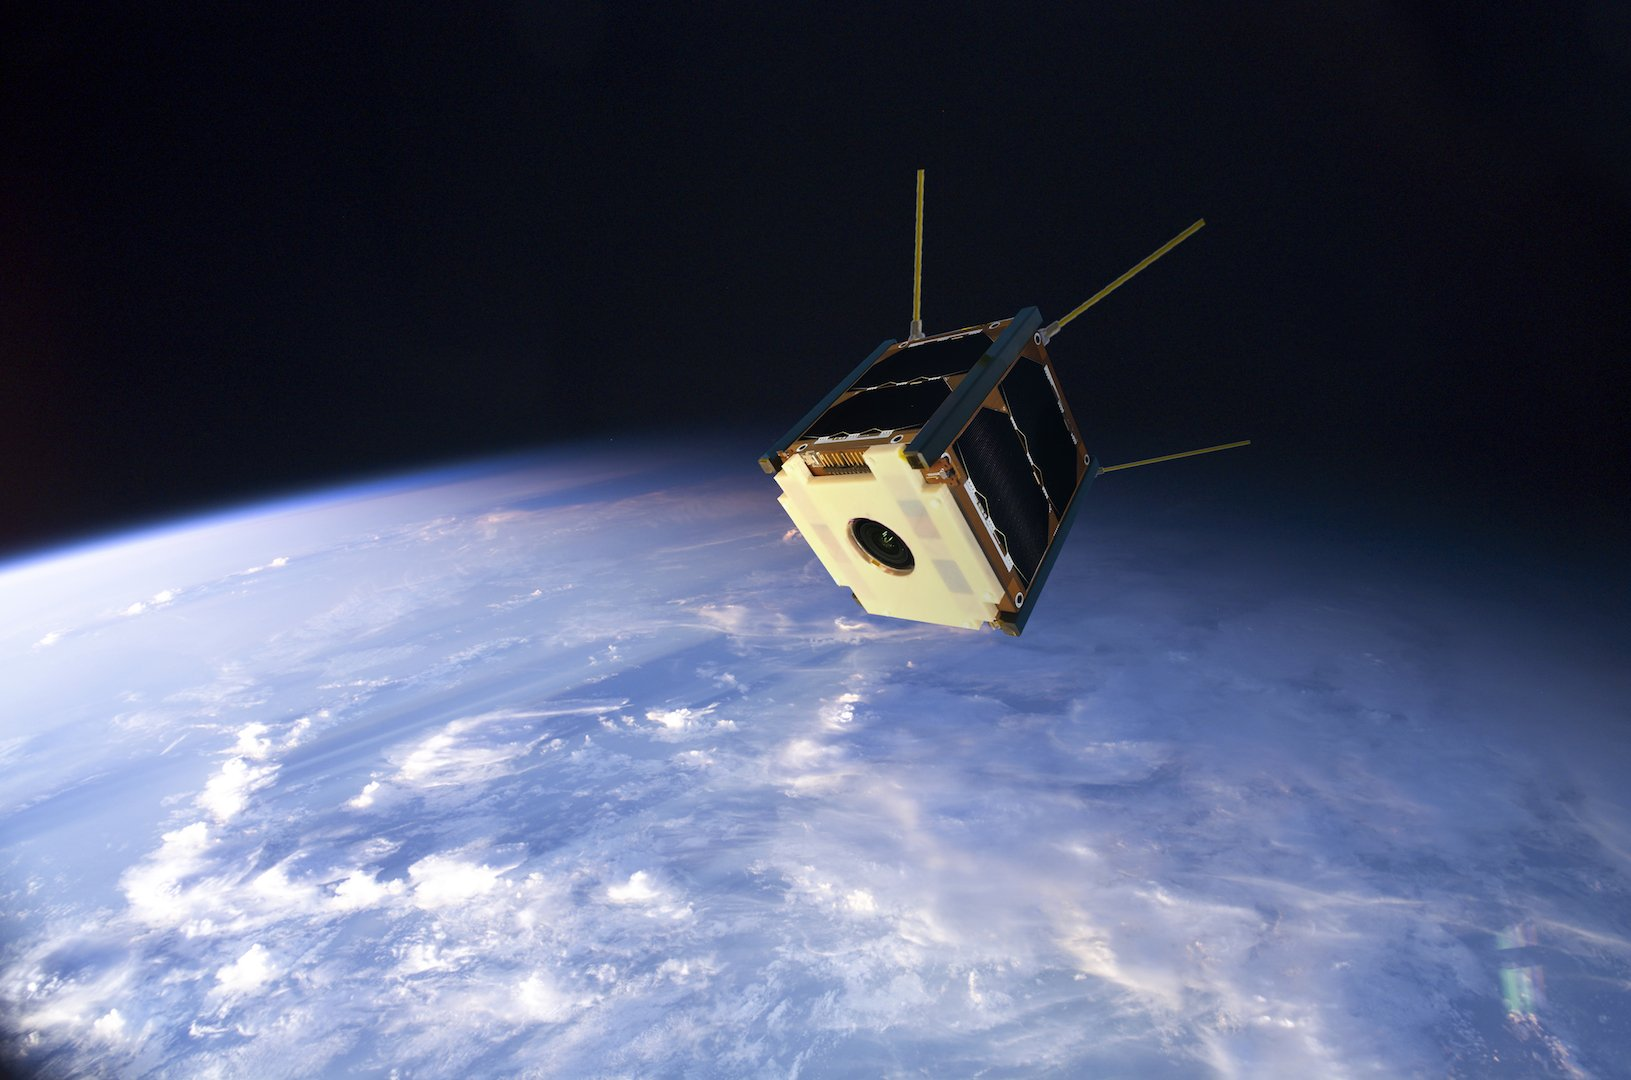
\includegraphics[scale=0.2]{s100_orbit}
\caption{Depiction of Suomi100 satellite in space. Courtesy of Jari Mäkinen. \cite{s100blogi}}
\label{s100intro}
\end{figure} 
\subsection{Research purpose and goals}
The aim of this thesis is to investigate \textit{how to carry out
functional system integration testing in order to improve CubeSat reliability}. Further, we wish to perform the testing in a systematic manner. By using software tools for automation of the testing, we can achieve a certaing degree of rigour and a systematic approach to testing. Similarly, verification tests for mechanical stress required by the CubeSat standard are done systematically in an automated fashion \cite{cds}. It would also be preferable that the functional system tests could be performed automatically in a systematic manner.\par 
From the technology point of view, the goal will be achieved by developing new generic and reusable function library with \textit{Python} programming language which can be used with the \textit{Robot Framework} \cite{robotmain} along with appropriate test suites and test setups.\par 
\subsection{Main questions and problems}
The main problem analyzed in this thesis is the unreliability of CubeSats, which the thesis tries to partly solve from the standpoint of system integration testing. The main question is, firstly, could this type of testing detect unrecoverable failures in the satellite operation and system integration, and, secondly, could we, in addition verify that the satellite fulfills its functional requirements?
\subsection{Outlining the scope of research}
In this thesis we study the use of one industry-proven automated acceptance framework to carry out the automated functional testing on Suomi100 and investigate the use of certain space-industry proven testing philosophies and methodologies into functional system integration testing with CubeSats.\par
In conjunction with the space industry test methodologies, we attempt to some degree simulate the environment related to functional operations of the satellite. In addition, we require that the simulation has to take into account the relatively small funds of university-led CubeSat projects.\par
%% Esimerkki luettelosta. Lyhyt ajatusviiva on k\"ayt\"oss\"a
%% luettelossa, ja se on pituudeltaan
%% en dash. Merkit\"a\"an latex-koodissa --. 




%% Opinn\"aytteess\"a jokainen osa alkaa uudelta sivulta, joten \clearpage
%%
%% In a thesis, every section starts a new page, hence \clearpage
\clearpage

\section{Background}
%\section{Aikaisempi tutkimus}
\subsection{CubeSat failures}
The CubeSat project was started in 1999 in Cal Poly \cite{cds}. Over 100 universities and other organisations have since contributed to the project. The purpose of the project is to provide a standard for the design of nanosatellites in order to decrease development costs and to make accessability to space easier \cite{cds}. In fact, the number of launched CubeSats has increased quite dramatically over the past few years \cite{Swart2016}, and it has been estimated that the number of CubeSat missions will increase in the coming years \cite{SpaceWorks2017}. Nevertheless, a large portion of these missions have failed due to various reasons \cite{Swart2016, Swart1, Swart2015}. The most common reasons include communication being lost with the satellite, batteries not recharging and the OBC not restarting, with an average of only 20 \% of missions being able to complete their full missions \cite{Swart2016}. \par 
\subsubsection{The CubeSat satellite specification}
The CubeSat project defines a CubeSat to be a nanosatellite with dimensions of ${10 \textrm{ cm} \times10 \textrm{ cm} \times{10} \textrm{ cm}}$ and with a mass up to 1.33 kg \cite{cds}. A satellite of this size is considered to be a 1U CubeSat. These units can be stacked together to form larger CubeSats, with some satellites consisting of even 12 units. A stack containing three units appears statistically to be the preferred size for a CubeSat \cite{Swart2016}. \par
Another important part of the concept is the \textit{Poly Picosatellite Orbital Deployer} (P-POD), which is a Cal Poly’s standardized CubeSat deployment system \cite{cds}. This deployment system is integrated with the launch vehicle and the springs in the system release the nanosatellites into space \cite{cds}. Usually a launch vehicle carries some primary payload, which is much larger than the CubeSats \cite{nasacubesat1}. If an extra weight can be launched along with the main payload, then the deployment pods with the CubeSats contained inside are integrated into the launch vehicle as secondary payloads \cite{nasacubesat1}. \par 
Although these nanosatellites are considerably smaller than most "traditional" satellites, they nonetheless are able to perform the regular operations of a satellite \cite{openorbiter}. As the classification, \textit{nanosatellite} defines, CubeSats are satellites in miniature size. Even though smaller, the same general class of subsystems are part of CubeSats as they are part of larger satellites \cite{openorbiter}. Subsystems containing electronics usually follow \textit{PC/104} standard which defines form factor and computer bus \cite{reliabilitycubesatelbus}. A single subsystem in a CubeSat can fit into one \textit{Printed Circuit Board} (PCB) following the PC/104 standard \cite{reliabilitycubesatelbus}.
Figure \ref{s100cad} illustrates the internal structure of Suomi100 CubeSat and the different subsystems that are integrated into the satellite.\par 
\begin{figure}[!h]
\centering
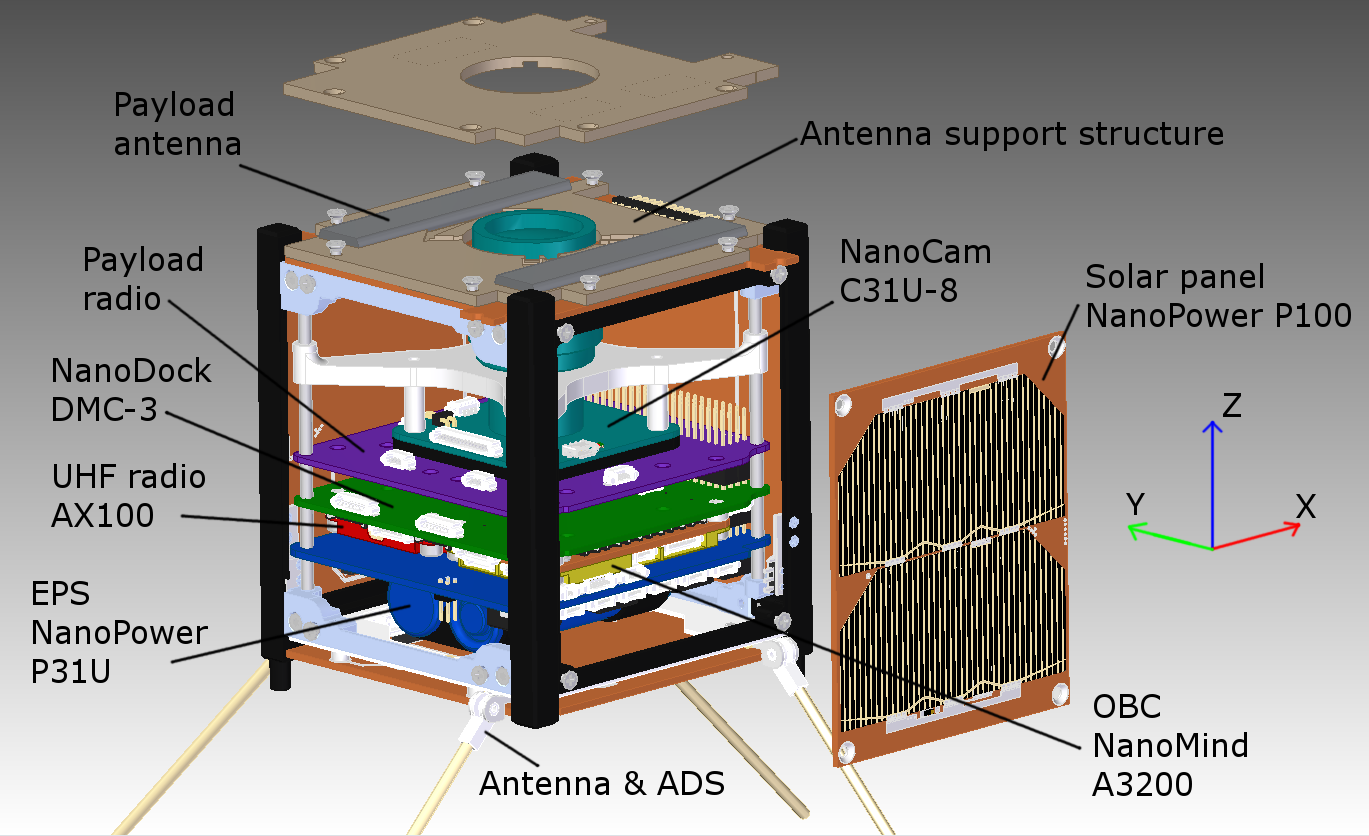
\includegraphics[scale=0.2]{s100cad}
\caption{Depiction of Suomi100 satellite subsystems. Courtesy of Aalto University.}
\label{s100cad}
\end{figure}  
From this Figure we can identify five subsystems that are common to all satellites. Power to the satellite is produced by the \textit{Electric Power System} (EPS) and this subsystem consists of the solar panels and batteries in the satellite. Additionally, the subsystem usually has some power regulation and power distribution features along with some features for reliable power production and storage \cite{spacesystemsengineering}.\par 
The central computer of the satellite is called the \textit{On-Board Computer} (OBC) and the task of this subsystem is to orchestrate the operation of all the other subsystems. In addition, the processing of commands received from the \textit{ground station} and the routing of them to the appropriate subsystem is the task of the OBC. \cite{spacesystemsengineering} \par 
The \textit{Communication system} (COM) is responsible for communication with the ground station. This subsystem usually has a computer of its own for processing the received radio signals. The antennas are also part of this system. Besides receiving and processing commands from the groundstation, \textit{Housekeeping} (HK) telemetry of the satellite system is commonly broadcasted in order to inform the groundstation about the state of the system. A satellite \textit{Beacon} is a specific type of broadcasted telemetry which is used to obtain the location of the satellite as well as its state in general.   \cite{spacesystemsengineering} \par
The proper orientation of the satellite is controlled by the \textit{Attitude Determination and Control System} (ADCS). For CubeSats, the orientation can be controlled either by mechanical reaction wheels, magnetorquers or by some other methods. The purpose of this system is to keep track of the orientation of the satellite and to change it according to commands received from the ground station. \cite{spacesystemsengineering}\par 
In addition to these subsystems, the \textit{Support Structure} forms the subsystem which integrates all of the subsystems into a single mechanical structure \cite{spacesystemsengineering}. The CubeSat standard defines the dimensions and materials for the support structure \cite{cds}. \par 
The groundstation in itself forms another element in the entire satellite system \cite{spacesystemsengineering}. As noted, communication with the satellite occurs via the groundstation. The station tracks and monitors the satellite and all the necessary information from the satellite is downloaded to the station. A groundstation consists of hardware elements such as antennas, power amplifiers and other radio components \cite{radiohandbook}. A computer is connected to the hardware elements and a groundstation software on the computer is used to control and track the satellite \cite{spacesystemsengineering, radiohandbook}. Pictures of the groundstation in Aalto University are presented in Figure \ref{aaltogs}.
\begin{figure}[!h]
\centering
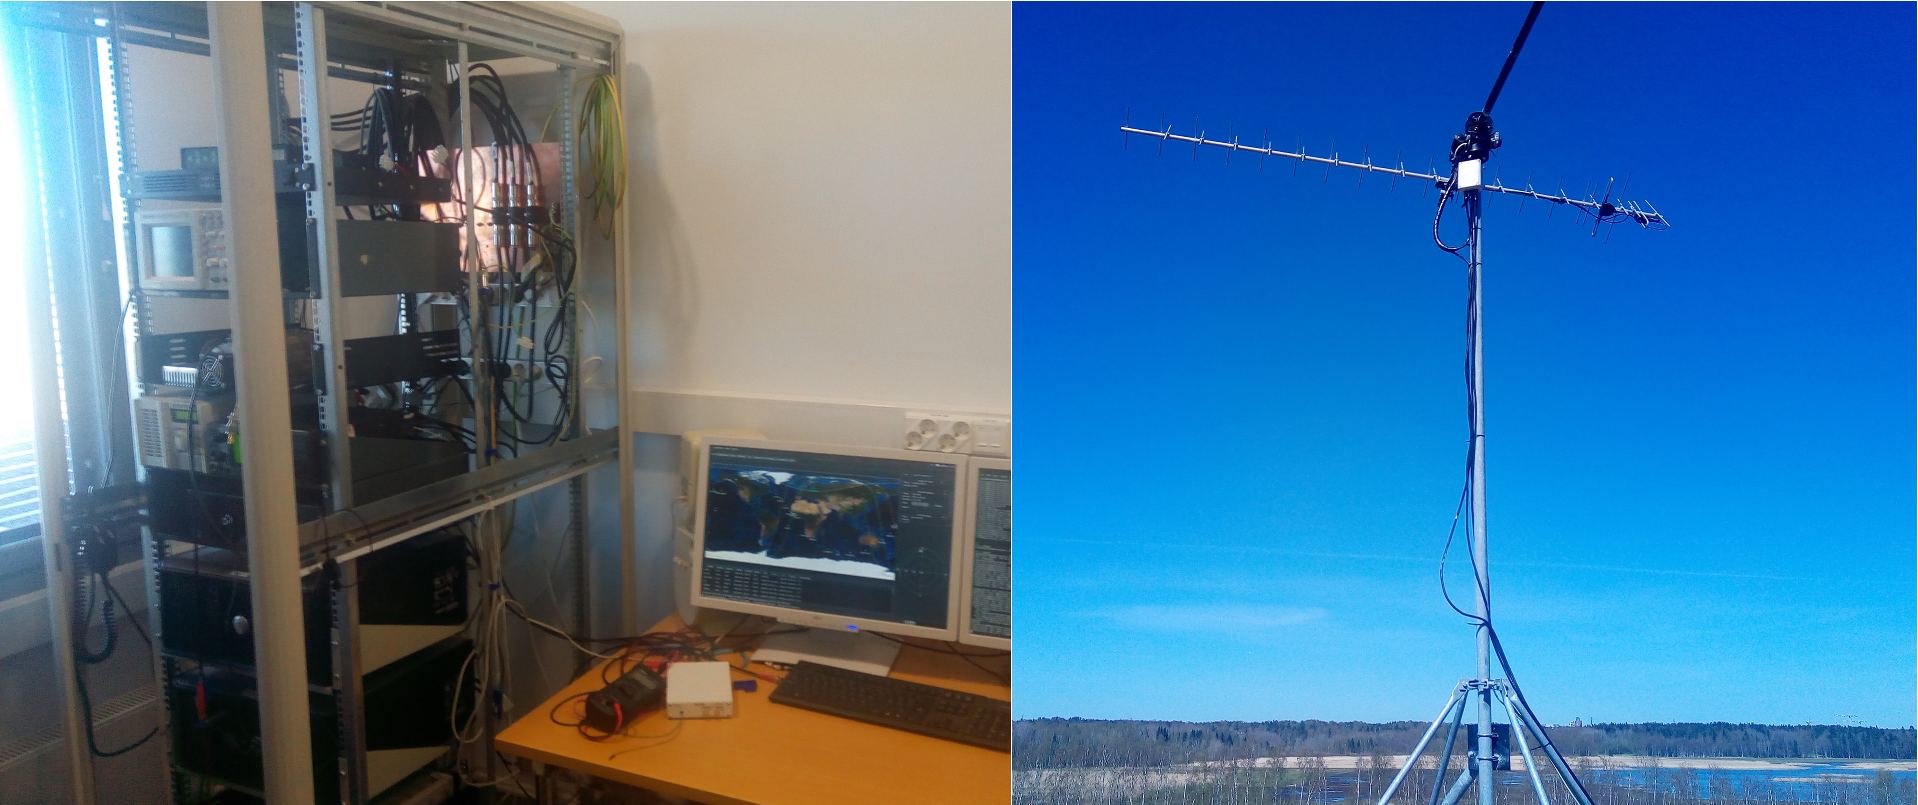
\includegraphics[scale=0.2]{groundstation}
\caption{Satellite groundstation in Aalto University. On the left in the image a computer is running the satellite control and tracking software. Certain radio hardware elements are present as well. The antenna used for controlling Aalto-1 satellite is on the right in the picture.}
\label{aaltogs}
\end{figure}  
    
\subsubsection{Failure rates of CubeSats}
Over 600 CubeSats have been launched as of 2017 \cite{Swart2017kalvo}. Some studies in recent years have been carried out to investigate the statistics of flown CubeSat missions. These studies looked for the percentage of failed missions and which subsystems contributed to each failure. Out of these failures, the amount of \textit{dead on arrival} (DOA) missions, where the satellite was never even able to be contacted from space, were also identified. The most active contributor to this topic has been Michael Swartwout and the representation of statistics of CubeSat failures in this thesis is based mainly on his work \cite{Swart2016, Swart1, Swart2015}, as not too many papers have yet been published on this issue.\par 
A study entitled \textit{The First One hundred CubeSats: A Statistical Look}, that was published in 2013, identified the failure rate for the first 100 flown CubeSats. Out of these first CubeSat missions flown between the years 2000-2012, a total of 34 had failed. From these failures, a third were never able to be contacted after they were released into space (DOA cases). Since then, many CubeSats have flown with varying degrees of success \cite{Swart2016}. Figure \ref{100first} shows the mission statistics for all CubeSats flown until 2017 \cite{csdatabase}. The different colours show at which state a CubeSat mission is or to which state the mission ultimately reached. \par
\begin{figure}[h!]
\centering
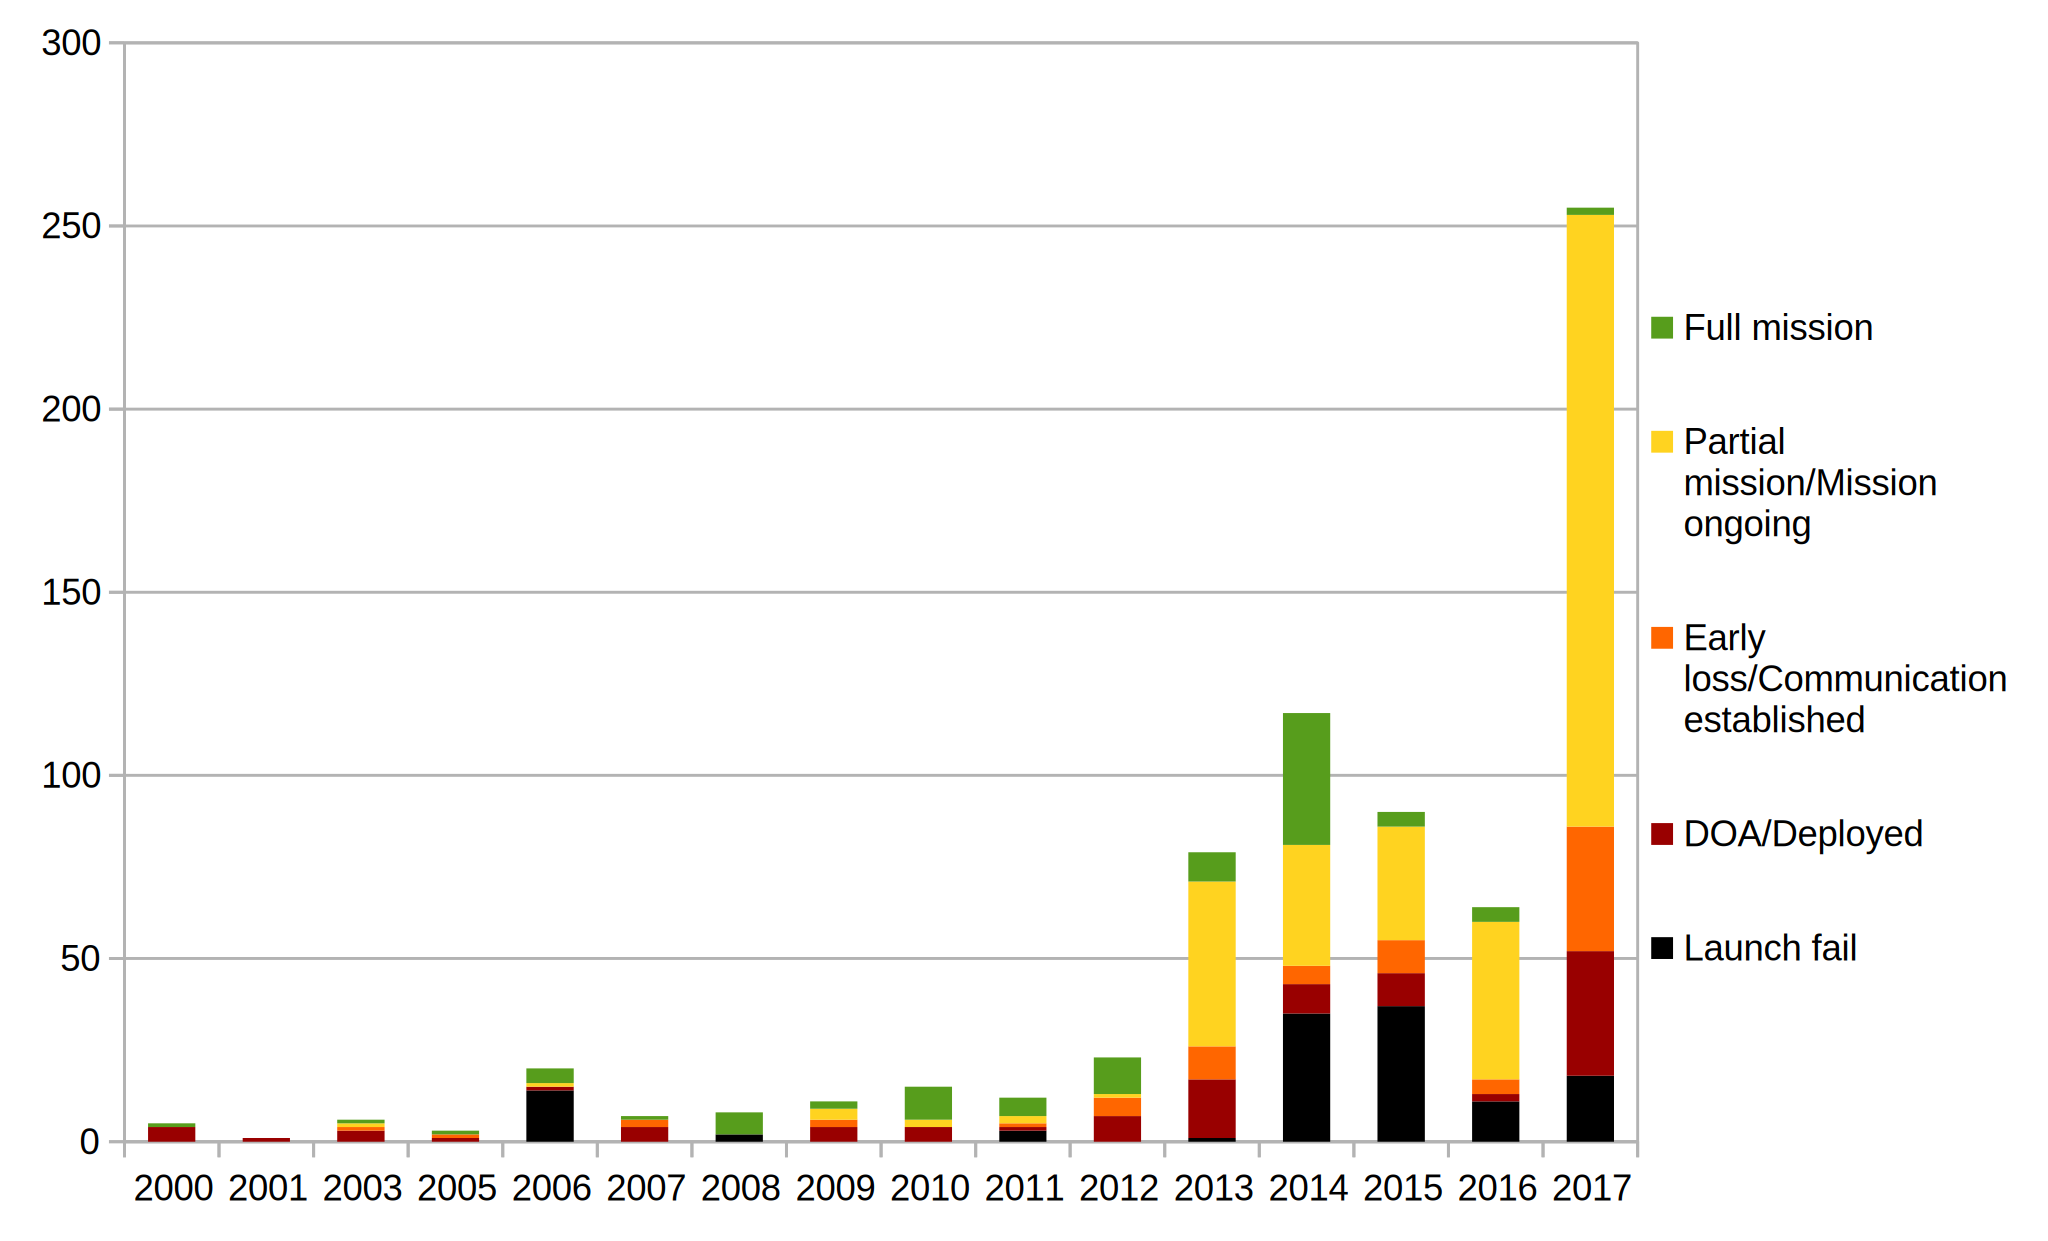
\includegraphics[scale=0.6]{cfdnew}
\caption{Mission statistics for CubeSats flown until 2017. \cite{csdatabase}}
\label{100first}
\end{figure} 
In order to break down and investigate the statistics, Swartwout has been continuing yearly to publish papers about the statistics of CubeSat failures, as new missions are flown each year \cite{Swart2016, Swart2015}. A study published in 2016, \textit{Secondary Spacecraft in 2016: Why Some Succeed (And Too Many Do Not)}, identified out of all CubeSats flown between 2000-2015 that reached orbit, 21 \% were DOA cases, and 9.8 \% were cases where the spacecraft was lost early in its life. When a CubeSat was lost early in its life, this means that communication with the satellite was established but no primary operations could be executed. When breaking down the statistics to categories based on the type of satellite and mission developer (new university teams, traditional contractors, experienced university and government teams, constellations), it was found that for the new university teams flying their first satellite, the failure rates were as follows: 44.1 \% DOA, 16.2 \% early loss and 16.2 \% mission success. On the other hand, for the CubeSats built by traditional contractors with established practices for integration and testing the numbers were: 6.3 \% DOA and 6.3 \% early loss. This DOA failure rate, however, halved when the new university teams, educated by their first failure, flew their second satellite. \cite{Swart2016, Swart2015}\par 
Figure \ref{hobbyistflown2015pic} below shows the statistics of failures for CubeSats between 2000-2015 flown by new university teams sending their first satellite, excluding those missions where the satellite was lost due to launch failure.\par 
\begin{figure}[h!]
\centering
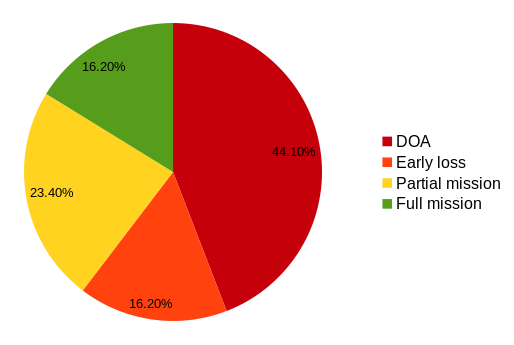
\includegraphics[scale=0.5]{university2015}
%\includesvg[]{images/university2015svg}
\caption{Statistics for CubeSats flown between 2000-2015 that were constructed by university teams without prior experience of satellite construction. \cite{Swart2016}}
\label{hobbyistflown2015pic}
\end{figure} 
For contrast, same statistics for CubeSats built by traditional contractors is shown in Figure \ref{tradiotionalflown2015pic}. A clear difference in DOA and early loss missions is visible for these two different groups.\par
\begin{figure}[h!]
\centering
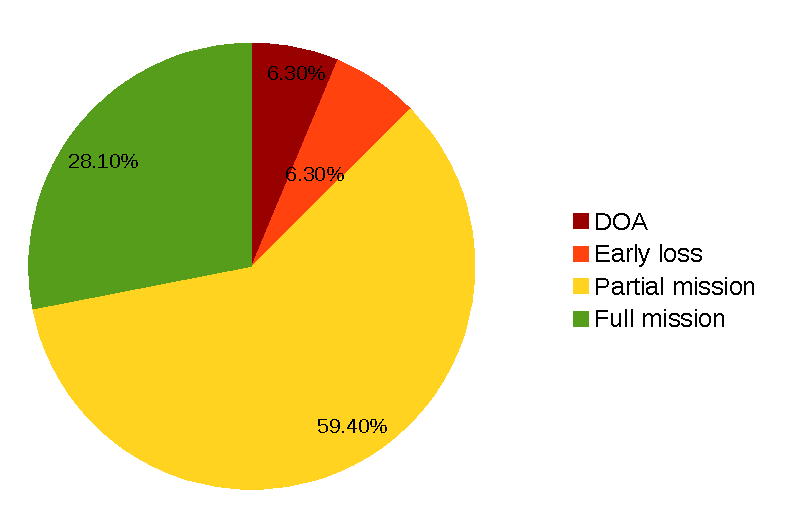
\includegraphics[scale=0.5]{traditional2015}
\caption{Statistics for CubeSats flown between 2000-2015 that were constructed by traditional contractors with extensive experience of satellite construction. \cite{Swart2016}}
\label{tradiotionalflown2015pic}
\end{figure} 
\subsubsection{Contribution of different subsystems to satellite failures}
Swartwout studied also the contribution of different subsystems to CubeSat failures in the paper \textit{The First One hundred CubeSats: A Statistical Look} \cite{Swart1}. The subsystems that were thought to be the cause of the failure were identified as follows: a configuration or interface failure between communications hardware (27\%), the power subsystem (14\%) and the flight processor (6\%), or the COM, EPS and OBC subsystem. A failure in a subsystem means in this context that the whole satellite is lost due to the failure. A failure in the OBC can mean, for example, that the processor fails to restart anymore or gets unrecoverably stuck in some way. For EPS the error can mean, for instance, that power is not being transferred to the satellite from the solar panels, and failure in the COM subsystem can imply, for example, that there is insufficient power for the antennas to close the link with the ground station.  \cite{Swart1}\par
Based on the beliefs of the satellite developers about the causes of failures, another study was carried out by Langer et al. in 2014 \cite{Langer} to investigate in more detail the contribution of different subsystems in CubeSat failures. This study by Langer also used the statistical data of CubeSat failures obtained from the \textit{CubeSat Failure Database} (CFD), at that point comprising data of about 178 CubeSat missions. With this data a reliability estimate for different subsystems was calculated using a \textit{Kaplan-Meier estimator} for nonparametric and parametric analysis. In addition, a parametric model for total CubeSat satellite reliability was devised. Figure \ref{subsystemfailures} below depicts the subsystem contributions to satellite failures for the first 178 CubeSat missions. Three main subsystems causing failures were identified in order of importance: EPS, OBC and COM, in accordance with Swartwout research, but with different percentages as EPS being the main contributor to failures \cite{Langer, Swart1}. \par
\begin{figure}[h!]
\centering
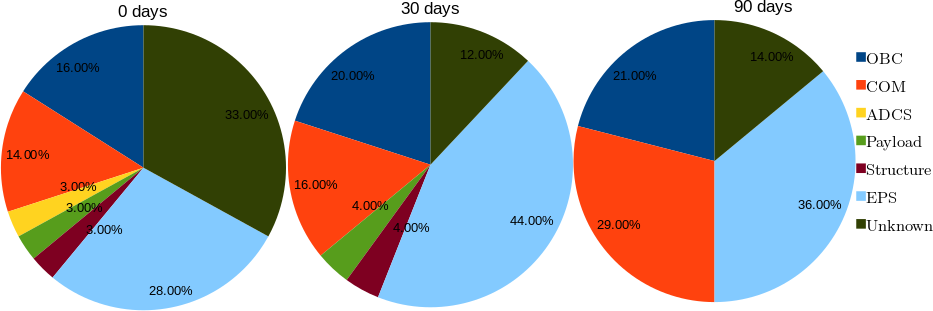
\includegraphics[scale=0.5]{subsystemmerge}
\caption{The beliefs of developers on the contribution of different subsystems to satellite failure. From left to right the charts present failure contribution data for 0, 30 and 90 days after launch. \cite{Langer}}
\label{subsystemfailures}
\end{figure}  
The statistical data gathered from questionnaires sent to 987 satellite developers (with 113 returned fully completed) showed that there was a belief that within the first six months there was a 50 \% chance that the satellite would fail. However, the beliefs of the developers seem to be too optimistic when compared to the data gathered from CFD. Nonetheless, from the subsystems having the greatest and least likelihood of causing system failure, the main subsystems were identified in the order: COM, EPS and OBC. \cite{Langer}\par
\subsubsection{Needs for the system level functional testing}
The aforementioned studies made some anecdotal guesses to what could have contributed to the failures in the satellites, ensuring that the missions failed either partially or completely. Though the current data does not clearly prove these educated guesses, it is believed by Swartwout and others that system integration level functional testing of the satellites has been lacking completely or has been inadequate \cite{Swart2016, Langer, Swart1, Swart2015}. \par
Based on his study in 2013, Swartwout came to a strong belief that the critical failures in the subsystems were caused by poor system integration. Notably, out of first 30 identified DOA cases, 24 were CubeSats made by university teams. In addition, based on his discussions with project managers and faculty leaders, it was noted that university teams constructing CubeSats have the misconception that the satellite works as expected the first time it is assemled together and thus no system integration level functional testing is performed. In the study, it was believed that operational tests demonstrating a \textit{"Day in the life of the satellite"} would be just as necessary as the vibrational tests to certify a CubeSat ready for launch. In addition, testing of recovery from resets, power management, startup sequences etc. would be important operations for the satellite to test. \cite{Swart1} \par
In later papers Swartwout has been less reluctant to make these claims directly, yet still identifying the large number of failed CubeSat missions coming from university-led satellite teams \cite{Swart2016, Swart2015}. As an example, the ORS-3 mission flown in 2013 consisted of 28 secondary payloads, and 13 of these payloads were assembled by new university teams flying their first satellite, and 15 were constructed by traditional contractors \cite{Swart2016}. While almost all (11 out of 13) of the university-built CubeSats failed, only one CubeSat built by a traditional contractor failed. Furthermore, all of these satellites had to go through the same vibrational and thermal tests and, in addition, were subject to mission-readiness reviews by the \textit{National Aeronautics and Space Administration} (NASA) and/or \textit{Department of Defense} of United States. Thus, some practices applied by the experienced contractors in satellite development were most probably missing from the university-built CubeSats.\par
In addition, David Voss of the \textit{Air Force Research Lab} speaking more recently at the 31st Annual Conference on Small Satellites held on 7th of August 2017 about CubeSat reliability said that, based on his experience with student and other small satellite projects, a core set of tests for power, communication and other subsystems would be needed \cite{smallsatconf31}. Furthermore, Michael Johnson, also a participator in the aforementioned conference and chief technologist at NASA's \textit{Goddard Space Flight Center} has been since 2017 working at NASA on making a reliability iniative to determine the best ways to improve CubeSat reliability \cite{smallsatconf31, ssvi}. He noted though that the goal is not to apply the same rigorous assurance procedures used earlier in larger and more expensive spacecraft, but to design new procedures and keep some of the older methods that can be useful. \par 
\subsubsection{Comparison of CubeSat failures to failures with larger spacecraft}
Besides CubeSats, failures have happened to more traditional spacecraft as well. In fact, the history of the space industry as a whole is filled with examples of failed missions \cite{failureshistory}. As an example, in recent years several Mars landers have failed during the landing phases of the mission \cite{marsfailures}. For instance, Mars lander \textit{Schiaparelli} crashed on the Martian surface in 2016 when a sensor used to measure the distance to the ground read a negative value and shut off its descent thrusters \cite{schiaparelli}.\par
Earlier research about the on-orbit failures was carried out in 2005 \cite{onorbitfailures}. It investigated failures of 129 different spacecraft between the years 1980 and 2005. The study found that there were many cases where the spacecraft failed early during its mission. Majority of the failures were caused by failures in the ADCS and EPS subsystems. The investigation concluded that among improved redundancy and flexibility in system design, adequate testing on ground could as well mitigate these failures as it was noted that the early failures could have been caused by inadequate testing and inadequate modeling of the environment where the spacecraft operates in. These conclusions in fact seem to be similar to what some of the surveys done on CubeSat failures indicate. \cite{onorbitfailures} \par
A research conducted in 2008 analyzed the contributions of different subsystems in the failures of 1584 satellites that were launched between 1990 and 2008 \cite{satsubsystems}. Solar array deployment and failure in the communication system were the major contributors to satellite failures for satellites that failed before 30 days after launch. After much longer operation period (i.e. years), the main subsystems contributing to failures were identified to be the ADCS and COM. Some similarity to the subsystem failures with CubeSats can be drawn here, with the communication subsystem and the solar panels playing a crucial role in the infant mortality of CubeSats.\par 
Further indication for the need of extensive testing was found after NASA initiated in the 1990s a more streamlined verification strategy based on the best commercial practices, commonly known as \textit{"Faster, Better, Cheaper"} \cite{satverplanning}. This led to poor results with commercial satellites that were launched during that period and a return to the more rigorous specifications and standards was expressed \cite{satverplanning}. In addition, a study conducted during this period in 1999 called \textit{"When Standards and Best Practices Are Ignored"}, found that out of 50 major space system failures 32 \% were related to inadequate verification and test processes \cite{whenstandignored}.\par 
In conclusion, based on the experiences found by the traditional space industry, the allegation that many CubeSat failures are due to poor testing at system integration level could be correct.\par 
\subsection{Satellite testing}
Satellites and many other spacecraft can be classified as \textit{embedded systems} \cite{embeddedjokusatellite}. An embedded system is defined in \textit{Real-Time Systems Design and Analysis: Tools for practitioner} as \textit{"A system which contains one or more computers (or processors) having a central role in the functionality of the system, but the system is not explicitly called a computer"} \cite{sularikurssi}. Systems such as these can contain  many parts and consist not just of software but of hardware elements as well \cite{embeddedsofteng}.\par
The testing of embedded systems has thus to take into account software testing as well as hardware testing and the interplay of software and hardware \cite{embeddedsofteng}. For example, mechanical stress and thermal vacuum tests are required by the CubeSat standard to be performed for CubeSats before launch \cite{cds}. Presenting different methodologies into hardware testing is out of the scope of this thesis as the topic of research is functional testing at system integration level. Performing a test such as this is, in practice, testing the software in the final hardware environment \cite{embeddedsofteng}. The general methodologies and practices used in software testing as well as some testing practices used by the traditional space industry are presented in this section.\par   
%Why do we talk about software testing? Because talk about that in this section
%Since 1970s, testing has been considered as a specific branch of software engineering \cite{artofsofttesting, compinspace}. More advanced techniques and methods for testing have been developed over the decades \cite{artofsofttesting}. For example, 
%NASA has contributed to the practices used in software testing through its efforts in the Apollo program \cite{compinspace}. \par
\subsubsection{Practices for software testing}
First a relevant question, \textit{why do we need to perform testing?} One reason is that humans make errors and often make optimistical assumptions about their work. Another aspect would be to call testing as a method of proving that the \textit{System Under Test} (SUT) works as we want it to work. Just as  a scientist carries out experiments to prove his theory, so too testing is done to prove that the system works as expected. A system in the context of testing can refer to anything from a single software function to entire operating system of a spacecraft. \cite{testingcomplex}\par
Another important aspect of testing is to find defects in the system and to recognize where they exist so that they can be corrected effectively \cite{sularikurssi, artofsofttesting}. A book by Glenford J. Myers titled \textit{The Art of Software Testing}, defines software testing as \textit{"Testing is the process of executing a program with the intent of finding errors"}, which is a general enough definition to contain many aspects of software testing \cite{artofsofttesting}.
\begin{center}
\textbf{Methods of testing}
\end{center}
Various different methods for software testing exist. So called box approach is one common method for testing \cite{sularikurssi, artofsofttesting}. Testing can either be done automatically by some computer-run script or manually by a tester who follows a specified test plan. 
Some of the testing methods are explained in the following pages in more detail.\\
%Test-case jutuista ja test-suite from art of software testing, chapter 4 test-case design. Chapter 6 higher order testing.\\ 
\\
\textbf{Black box testing}\\ 
Black box testing is performed with no knowledge about the internal structure of the SUT, which can be a single function of a software or a whole operating system for example. A select set of inputs are given to the system and from the outputs we see how the system performed. If the outputs were what we expected, the system passed the test. Black box testing is usually used when we are interested in the outward functionality of the SUT. Figure \ref{boxfigurespuge} below illustrates black box testing method. \cite{artofsofttesting}\\ 
\\
\textbf{White box testing}\\ 
White box testing is performed when we are interested about the internal functionality of the SUT. Testing of the internal functions rather than the outwardly expected functionality is the goal of white box testing. Usually this type of testing is performed at the smaller component or unit level of the system. Figure \ref{boxfigurespuge} below gives an illustration of white box testing. \cite{artofsofttesting}\\
\begin{figure}[h!]
\centering
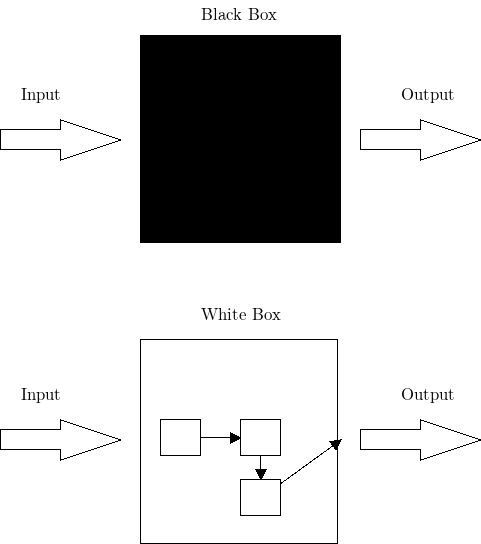
\includegraphics[scale=0.4]{whiteblackbox}
\caption{Illustration of black and white box testing methods. \cite{artofsofttesting}}
\label{boxfigurespuge}
\end{figure} 
\\
\textbf{Input selection}\\
There exists different methods for choosing the appropriate inputs for testing. With \textit{exhaustive testing} all possible input combinations are investigated, which usually leads to combinatorial explosion, and the testing of all of them can, in some cases, even take millions of years. \textit{Boundary-value testing} and \textit{Equivalence partitioning}, for example, solve this issue by having a logical set of combinations and not all possible ones. \cite{artofsofttesting}\par 
Another approach in choosing the right inputs is to look for the requirements and specifications defined for the software \cite{artofsofttesting}. Especially for higher-level testing this approach is preferred. The set of inputs can in such cases also be derived from specified \textit{user  documentation} of the program, which defines how the program is to be used and what are the effects of the actions performed \cite{artofsofttesting}. A single \textit{use case} describes how to use the system in order to reach a particular goal \cite{sularikurssi}. In other words, a use case is a description of an operational scenario of the system.\\
\\
\textbf{Test case}\\
A set of inputs along with the test preconditions and expected results form a \textit{test case}. The purpose of a test case is to drive the execution of a testable item to meet the objectives defined for the test case, such as verifying proper implementation, detecting errors and so forth \cite{ieeesofttesting1}.
A collection of test cases with the focus on testing a specific area of a system is referred to as a \textit{test suite}.   
\begin{center}
\textbf{Levels of testing}
\end{center}
Testing can be carried out at different levels of the system and at each level we investigate different aspects of the system. Usually testing of an entire software program is performed by starting from smaller parts and gradually moving to the larger components of the system \cite{sularikurssi, testingcomplex}.
One can define different levels of testing as follows \cite{sularikurssi, artofsofttesting, ieeesofttesting1}:\\ 
\\
\textbf{Unit testing}\\ 
Unit testing of software is the most basic level of testing. On this level, individual components of a software program are tested separately. For example, testing the outputs of a given software function is considered a unit test. Usually these tests are written or performed by the person who also wrote that particular part of the software. Black box and white box methods are usually applied for unit tests. Inputs for test cases are commonly derived by using some of the methods for input combination, such as equivalence partitioning.
\\
\\
\textbf{Integration testing}\\
Integration testing tests the functionality of larger software components, consisting of several smaller units. With this level of testing we ensure that the smaller units interact with each other properly and that the biggest component itself works properly. Both black box and white box methods can be applied to carry out the tests. Inputs for test cases are commonly derived in the same manner as with unit testing.
\\
\\
\textbf{System testing}\\ 
On this level, testing is done on a complete integrated software system to see whether it conforms to the requirements specified for it by the development team. With this testing, we see whether the integrated parts of the software work together and also see how the whole system functions. Black box testing is usually applied at this level. The test cases derive their inputs with some of the methods specified for higher level testing. For example from documented use cases of the system.
\\
\\
\textbf{Acceptance testing}\\ 
At this level testing is usually performed by some outside team that had no involvement in the development of the software. This team could be specifically selected final users or there could be a separate testing team to ensure that the final product conforms to the original requirements defined by the orderer of the software. Black box testing methods are applied at this level. The test cases derive their inputs with some of the methods specified for higher level testing. The more commonly used method is to derive the inputs from the documented use cases of the system.
\\
\\
\textbf{System integration testing}\\
In the interest of embedded systems, system integration testing is performed to test the overall embedded system assembled from sub-components once the sub-components have passed the previous testing levels. System integration testing is performed to verify that the integrated system meets its requirements and for one to detect any issues emerging when the sub-systems are brought together. Black box testing is used to perform this testing. Some of the methods specified for higher level testing are used to derive the inputs for the test cases. \cite{embeddedsofteng, systinttesting1}\\
\begin{center}
\textbf{Types of testing}
\end{center}
Besides the method and level of testing chosen, there exists multiple types of different testing that can be performed. \cite{sularikurssi, embeddedsofteng, testingcomplex}\par 
The most common ones are the following \cite{sularikurssi}:\\
\\
\textbf{Functional testing}\\
Functional testing is performed when we are interested in knowing what the SUT does based on the inputs to it. Black box testing methods are mostly applied here. Functional testing can be done at all levels of testing.
\\
\\ 
\textbf{Non-functional testing}\\
Non-functional testing on the other hand is interested in how the SUT operates, rather than what it actually does. Several different testing types can be considered to belong under this category, such as performance testing or security testing for example. Both black and white box methods can be applied to this type of testing.
\\
\\ 
\textbf{Performance testing}\\
Performance testing is done for the interest of knowning how stable and responsive the system is under a certain load. This testing can be done at all levels and the methods can vary.
\\
\\ 
\textbf{Regression testing}\\
Regression testing is usually performed after the software has changed from the previous version which had been tested. For example, when a new feature is added or some defects are fixed, regression testing is done to see whether the old parts of the software still work as expected. Usually a fixed set of unchanging test cases can be executed once every change has been made to the software.
\\
\\ 
\textbf{Smoke testing}\\
Smoke testing is carried out to verify that the most important parts of the system work properly. Usually the test set is small as we are only interested in seeing if anything fundamental is not working in the system.

\subsubsection{Space industry methodologies}
In testing of the satellite software at different levels, one has to take into account the effect of different system environments respective to the level of testing \cite{embeddedsofteng, softacceptancespace}. From simulating the target hardware on a computer to running tests on an integrated satellite, different methodologies exist to account for different environments \cite{softacceptancespace}. In addition, satellites consist of several subsystems (as described in section 2.1.1) and each can have their own software. The software of each of these subsystems is tested individually and finally together on the integrated satellite \cite{sularikurssi, softacceptancespace}.\par
%In the 1950s first man made devices were sent into space by the USSR and United States \cite{aftersputnik}. Since that time, space industry has seen a gradual growth with perhaps the biggest and most expensive endeavours being the manned missions to the Moon, the U.S. shuttle program and the International Space Station being funded by several nations \cite{nasacosts}. During the evolution of the industry, manufacturers have had to develop and improve the practices in software and hardware design and testing as the devices have become more complex and reliability has become an issue \cite{compinspace}. For example, software engineering as a specific branch of computer science emerged during NASA's Apollo program \cite{compinspace}.\par 
At NASA, at different levels of system development, different environments and different teams are used for testing \cite{softacceptancespace}. During the course of the Apollo program, NASA adopted the four-level software testing practice \cite{compinspace}. At the lowest level, unit and integration tests of software of a hardware component/subsystem are carried out by the software developers on a desktop environment. At the system and acceptance levels the tests are performed by developers and separate test engineers respectively. Simulators and \textit{testbeds} are used when testing the software at this level \cite{softacceptancespace, cassinitestbed}. This environment contains assembled subsystems, interface emulators and ground and flight software. The goal is to properly verify the required software functionality. As an example, a system testbed was used to test the operation of singular and several subsystems of the Cassini-Huygens space probe \cite{cassinitestbed}. Several inputs to the subsystems simulated the space environment while tests were being carried out. On the system integration level, the whole spacecraft is assembled and the integrated system is tested with different scenarios of satellite operation \cite{softacceptancespace, tor}. For example, downlink procedures, maneuvres, payload operations and so forth are tested at this level. This test is usually performed by a separate  integration test team \cite{softacceptancespace}. Figure \ref{testlevelchart} below describes the levels and methods of testing at different levels of spacecraft development. \par
\begin{figure}[h!]
\centering

\includegraphics[scale=0.8]{spacetestingnew}
\caption{Illustration of spacecraft testing on different levels of system development. \cite{softacceptancespace, tor}}
\label{testlevelchart}
\end{figure}
At the \textit{European Space Agency} (ESA) the preferred levels for testing of the spacecraft are equipment, subsystem, element, segment and overall system \cite{ecss}. ESA also states that a system verification by testing shall consist of testing of system performance and functions under representative simulated environments \cite{ecss}. As can be deducted, testing is done in a way similar to what is done at NASA. \par 
Emphasis on testing at the highest level of assembly or in other words, testing the whole assembled spacecraft has always been a NASA priority \cite{reliabilitylessonsfromnasa}. A mantra commonly used in the space industry has been \textit{"Test like you fly"} (TLYF), meaning that a spacecraft should be tested on ground in the same way as it would be operated in-orbit \cite{satverplanning, tor}.  In general, the TLYF philosophy provides a basis for acquiring and verifying a system and gives a mission-centric focus on space system validation and verification \cite{tor}. As such, the same software and hardware should be used in testing as that which will be used when the spacecraft is launched into orbit \cite{satverplanning}. One such test on system integration level using this philosophy is commonly referred to as \textit{"Day in the life"} or operational satellite scenario testing \cite{satverplanning, tor}. \par
In "Day in the life" testing, tests are derived from the mission operations requirements documents \cite{tor}. A document called \textit{operations concept document}, or CONOPS, is commonly referred for this type of documentation \cite{tor}. The focus with this testing is on verifying whether the space and ground segments can accomplish the mission as it was envisioned in these documents. The test involves having the integrated and assembled spacecraft on the ground being flown in a flight-like manner to the extent feasible. In addition, controlling and communicating with the spacecraft from the ground station is tested in the way that has been envisioned in the mission operations requirements document \cite{tor}. This type of testing has been deemed necessary as many failed space missions had actually been succesfully tested to meet all their requirements, but were not tested to verify succesful completion of mission objectives \cite{tor}. This test is required by NASA's Goddard Space Flight Center and ESA to be performed before a spacecraft can be verified for mission readiness \cite{tor, ecss}. \par
It has to be further noted, that space as an environment itself provides extra challenges for maintaining proper reliability of spacecraft. For example, variations in temperature as well as particles carried by the solar wind bring unique demands for reliable design. These devices operating practically out of our physical reach impose further demands for system reliability. If a satellite orbiting at an altitude of 500 km develops an unrecoverable processor error, there is no practical way for us to go there and physically press the reset switch to get the satellite operating again. Therefore, the testing of spacecraft has to be thorough and systematic. Higher demands are usually set for the testing of spacecraft than for terrestial systems. \cite{spacesystemsengineering} \par 
%Some testing standards.
%ESA ECSS-E-ST-10-02C.
%http://spacegrant.colorado.edu/COSGC_Projects/co3sat/Testing.htm
%NASA Systems Engineering steps and procedures (design reviews, SAR, SIR etc.).\par
%https://standards.nasa.gov/nasa-developed-standards
%https://www.esa.int/About_Us/Business_with_ESA/Space_Related_Standards2
\subsection{Test automation}
Software test automation has been a topic of interest among software projects for the past few decades \cite{testautomationconf2013}. It has been heralded as a solution for decreasing costs related to testing and enabling the release of human resources for other tasks \cite{workshopontestautomation, kasurinentesting}. Test automation can be performed on many levels of testing, from unit level to acceptance and beyond. It has been found to be most useful in automation of repetive tasks and in automating execution of repetive test cases \cite{kasurinentesting}. Several software tools and frameworks for test automation have been developed over the brief history of test automation \cite{testautomationconf2013, kasurinentesting}. \par 
\subsubsection{Test automation frameworks}
A test automation framework is an integrated system that sets the rules of automation for a specific product. This system integrates the function libraries, test data sources, object details and various reusable modules. When some changes are made to the system under test, only the test cases need to be modified. \cite{exploringuseofta} \par
A common practice is that test cases are written into separate scripts with a scripting language specific to the framework \cite{robotmain, exploringuseofta}. Function libraries are written into their own source code files with some of the more common programming languages such as Python, \textit{Java, C++} and so forth \cite{robotmain, modelbasedtesting}.
The test scripts then call for the functions in the function libraries to perform the actual automation \cite{modelbasedtesting}. For example, a script simulating a network system being used could call for functions in the function library to send commands over the network.\par 
%Several different test automation frameworks exist based on different types of test case generation techniques. Frameworks based on \textit{Keyword-driven} testing use keywords. Frameworks utilizing \textit{Data-Driven} testing use something else. In \textit{Model-Based} testing happens something [modelbasedtesting].\par
%https://en.wikipedia.org/wiki/Test_automation#Framework_approach_in_automation 
\subsubsection{Robot Framework}
Robot Framework is generic test automation framework for acceptance testing originally developed in Nokia Networks \cite{robotmain}. The framework emerged from a Master's thesis written by Pekka Klärck for one Finnish software testing consultancy company known as \textit{Qentinel Oy}. The title of his thesis was \textit{"Data-Driven and Keyword-Driven Test Automation Frameworks"} and it was written in 2005 \cite{robotmain, klerkdippa}. In turn, the writer of this thesis at hand has also been working at Qentinel and thus has become quite familiar with the Robot Framework. This is one of the reasons why the Robot Framework was chosen for the test automation of the Suomi100 satellite. \par 
Robot Framework is, in addition, open-source under the \textit{Apache 2.0} license, and the modularity of the framework allows people and companies to write their own testing libraries either with Python or Java. The core of the framework is implemented with Python. Instructions for installing the framework can be found from \url{https://github.com/robotframework/robotframework#installation}.
The modularity and flexibility of the framework has thus made it possible to use it to perform test automation on various different projects. Some companies such as \textit{ABB, Nokia, Kone, Metso, Axon, Zilogic} and others have used the Robot Framework in the testing of embedded systems. Other companies such as \textit{Finnair} have also been utilizing it to test their web based applications. Some companies such as ABB, Metso and others are performing their testing with the Robot Framework in many different areas. \textit{U.S. Naval research laboratory} has also been using the framework with their \textit{SAGE} multi-agent system. \cite{robotmain}\par 
Based on how many companies have been confidently using the framework \cite{robotmain} and that it has been used in many different areas (embedded systems, web applications, etc.), we feel confident to develop the test automation of the Suomi100 satellite with Robot Framework. In addition, the framework being open-source makes it even more appealing for this task \cite{robotmain}. Future CubeSat projects could use the Robot Framework as well and possibly also use the generic libraries that are created in this thesis.\par
Robot Framework uses a \textit{keyword-driven} testing technique and the test scripts have a tabular data syntax. With keyword-driven testing, the test cases consist of keywords and each keyword performs a specified action. The keywords in a Robot Framework test case are executed in order from top to bottom. The keywords themselves can be written to be fairly abstract sentences (which perform many different actions) or can be simple function calls (performing one action). Below in Figure \ref{robotexample} a Robot Framework test suite script is shown. \cite{robotuserguide}\par 
\begin{figure}[h!]
\centering
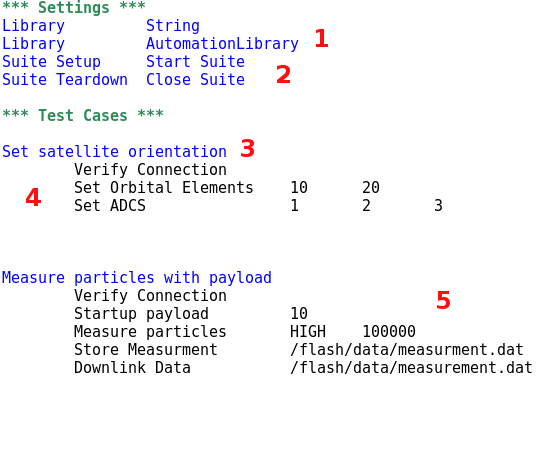
\includegraphics[scale=0.55]{robotexamplemod}
\caption{Example of a Robot Framework test suite with two test cases.}
\label{robotexample}
\end{figure}
In Figure \ref{robotexample}, the number (1) on the script shows how function libraries are included in the test suite. These libraries can simply be Python files or Python classes. In that case, a simple Python file can be included to the suite by defining a relative path and the filename. Python modules which are included in the operating system \textit{PATH} variable can be included without relative paths.\par 
Number (2) on the script illustrates how the test suite setup and teardown scripts are included. These calls to start and close the test execution can also be Python functions included in the function libraries. Call for \textit{Suite Setup} defines what operations are peformed at the start of the test execution, such as opening connection to the SUT, initiating  the system to a default state and so forth \cite{robotuserguide}. Calling for \textit{Suite Teardown} defines what actions are performed when test execution ends \cite{robotuserguide}, such as resetting and closing the SUT.\par 
Number (3) shows in what way the test cases are defined. The names of the test cases are arbitrary. However, they should be named differently from each other and the naming preferably should represent the activity of the test case \cite{robotuserguide}. \par 
The lines next to number (4) present how keywords are called. The keywords can be direct calls to Python functions or methods of the same name, or they can be other keywords defined in some Robot Framework script file. The underscores and letter cases in the Python function definition are translated so that the representive Python function can be called with the keyword in any way the keyword is written \cite{robotuserguide}. Spaces and letter cases do not concern the keyword when calling for a Python function from Robot Framework.\par 
Under number (5) the parameters for the representive keywords are defined. These parameters are separated from the keywords and from each other by arbitrary number of tabular spaces \cite{robotuserguide}.\par
When the script is executed, Suite Setup is first performed and then all the test cases in order from top to bottom are executed. If any keyword in a test case fails, the entire test case is counted as failed. Finally, Suite Teardown is called and the test execution log files are generated in \textit{Hypertext Markup Language} (HTML) by Robot Framework. Several Robot Framework log files can be seen in Appendix \ref{LiiteC}. \cite{robotuserguide}
\subsection{Suomi100 satellite mission}
The software programs related to Suomi100 satellite comprise the SUT in this thesis. The satellite mission was conceived in 2015 in the interest of celebrating Finland's 100 years of independence \cite{s1002015}. The original design called for a 2U CubeSat, but was later changed to a 1U CubeSat. The mission demanded having two payloads on board the satellite. The first payload is a white light camera for taking images of Finland from space, and the second payload is a science instrument which measures the radio static in the Ionosphere \cite{s100blogi, s1002015}.\par
\subsubsection{Mission requirements} 
The requirements and definitions for the mission are presented in this section. The satellite and its software are described in section 3.1. The first requirement defines the functional requirement of the mission as: 
\\
\textbf{\textit{"Take images of Finland and measure RF radiation caused natural and man-made sources."}}
\\
\\
Table \ref{suomi100functional} on the next page shows functional requirements derived from this requirement.
%\caption{Suomi100 functional mission requirements derived from the requirement to take images of Finland and to measure natural and man-made \textit{Radiofrequency} (RF) radiation.}
%\label{suomi100functional}
\begin{table}[!h]
\centering
\caption{Suomi100 functional mission requirements derived from the requirement to take images of Finland and to measure natural and man-made \textit{Radiofrequency} (RF) radiation}
\label{suomi100functional}
\begin{tabular}{|l|l|l|}
\hline
1st Derivation                                                                                                                                    & 2nd Derivation                                                                                                             & 3rd Derivation                                                                                                     \\ \hline
\multirow{4}{*}{\begin{tabular}[c]{@{}l@{}}Take 1 \\ image of \\ Finland \\ per day\end{tabular}}                                                 & \begin{tabular}[c]{@{}l@{}}Capable of pointing \\ camera towards Finland\end{tabular}                                      & \begin{tabular}[c]{@{}l@{}}Camera points with 5\\  degree accuracy\end{tabular}                                    \\ \cline{2-3} 
                                                                                                                                                  & \begin{tabular}[c]{@{}l@{}}Must compress images \\ for faster downlinking\end{tabular}                                     & \begin{tabular}[c]{@{}l@{}}RAW, BMP and JPEG \\ output formats\end{tabular}                                        \\ \cline{2-3} 
                                                                                                                                                  & \begin{tabular}[c]{@{}l@{}}Image resolution shall be \\ adequate to discern \\ geographical features\end{tabular}          & \begin{tabular}[c]{@{}l@{}}250 m / pixel \\ resolution\end{tabular}                                                 \\ \cline{2-3} 
                                                                                                                                                  & \begin{tabular}[c]{@{}l@{}}Must take images at both \\ day and night time\end{tabular}                                     & \begin{tabular}[c]{@{}l@{}}Polar orbit \\ (SSO noon/midnight)\end{tabular}                                         \\ \hline
\multirow{6}{*}{\begin{tabular}[c]{@{}l@{}}Capable of \\ measuring \\ entire frequency \\ range \\ at all \\ points over \\ Finland\end{tabular}} & \multirow{3}{*}{\begin{tabular}[c]{@{}l@{}}Payload capable of \\ measuring RF radiation \\ between 1 -10 MHz\end{tabular}} & \begin{tabular}[c]{@{}l@{}}1-10 MHz region \\ measured in 6 kHz strips\end{tabular}                                 \\ \cline{3-3} 
                                                                                                                                                  &                                                                                                                            & Sampling frequency 32-48 kHz                                                                                           \\ \cline{3-3} 
                                                                                                                                                  &                                                                                                                            & \begin{tabular}[c]{@{}l@{}}50 samples from \\ each 6 kHz band\end{tabular}                                         \\ \cline{2-3} 
                                                                                                                                                  & \multirow{2}{*}{\begin{tabular}[c|]{@{}l@{}}Adequate resolution \\ for scientific \\ measurements \end{tabular}}             & Radio resolution 16 bits                                                                                           \\ \cline{3-3} 
                                                                                                                                                  &                                                                                                                            & AGC resolution 5 bits                                                                                              
                                                                                                                                                  \\                                                                                                                                                                                                                                                                                   
&                                                                                                                                                  &                                                                                                                                                                           %\vline
                                                                                                                                                   
\\                                                                                                                                                  &
                                                                                                                                                  
&                                                                                                                                                 %\vline
                                                                                                                                                   \\ 
                                                                                                                                                   \cline{2-3} 
                                                                                                                                                  & \begin{tabular}[c]{@{}l@{}}Must compress data for \\ faster downlinking\end{tabular}                                       & \begin{tabular}[c]{@{}l@{}}Calculates summed value \\ of the 50 data points of \\ each frequency band\end{tabular} \\ \hline
\multirow{2}{*}{\begin{tabular}[c|]{@{}l@{}}Can \\ communicate\\  with \\ ground \\ station\end{tabular}}                                          & \begin{tabular}[c|]{@{}l@{}}Satellite sends and \\ receives\\  data via cubesat \\ space protocol\end{tabular}              & \multirow{2}{*}{\begin{tabular}[c|]{@{}l@{}}Ground station uses \\ Cubesat space protocol\end{tabular}}             \\ \cline{2-2}
                                                                                                                                                  & Software includes scheduler                                                                                                &                                                                                                                   
                                                                                                                                                  \\ 
                                                                                                                                                 &
                                                                                                                                                 &
                                                                                                                                                  \\
                                                                                                                                                  &
                                                                                                                                                  &
                                                                                                                                                  \\ 
                                                                                                                                                  &
                                                                                                                                                  &
                                                                                                                                                   \\
                                                                                                                                                  
                                                                                                                                                   
                                                                                                                                                    \hline
\end{tabular}
\end{table}
\\
The second requirement defines the operational requirement as:\\
\textbf{\textit{"Suomi100 is a CubeSat."}}
\\
\\
This requirement defines in general that Suomi100 must meet the requirements defined for the CubeSat standard and other operational performance requirements such as power consumption and downlink speed. For the interest of this thesis, going through them in detail is unnecessary. It is necessary only to note that Suomi100 meets the requirements set for the CubeSat standard, and that the requirements for power consumption and downlink speed are met. \par
%Table \ref{suomi100operational} below desribes the operational requirements for the mission.
%\begin{table}[!h]
%\centering
%\caption{Suomi100 operational requirements derived from the requirement that Suomi100 is a CubeSat.}
%\label{suomi100operational}
%\begin{tabular}{|l|l|l|}
%\hline
%1st Derivation                                                                                                                                  & 2nd Derivation                                                                                                                                      & 3rd Derivation                                                                                                                                                                                                                                                                                                                                                                                   \\ \hline
%\multirow{4}{*}{\begin{tabular}[c]{@{}l@{}}Satellite must meet \\ requirements \\ specified in \\ CubeSat design \\ specification\end{tabular}} & \begin{tabular}[c]{@{}l@{}}Must meet mechanical \\ requirements\end{tabular}                                                                        & \begin{tabular}[c]{@{}l@{}}Maximum mass 1.33kg. \\ Center of gravity located within \\ 2 cm from geometric center.\end{tabular}                                                                                                                                                                                                                                                                  \\ \cline{2-3} 
%                                                                                                                                                & \begin{tabular}[c]{@{}l@{}}Low out-gassing \\ materials\end{tabular}                                                                                & \begin{tabular}[c]{@{}l@{}}Total Mass Loss (TML) \textless 1.0 \%.\\ Collected Volatile \\ Condensable Material \\ (CVCM) \textless 0.1\%.\end{tabular}                                                                                                                                                                                                                                          \\ \cline{2-3} 
%                                                                                                                                                & \begin{tabular}[c]{@{}l@{}}Must meet electrical \\ requirements\end{tabular}                                                                        & \begin{tabular}[c]{@{}l@{}}Sat powered off while in PPOD.\\ The CubeSat shall include \\ an RBF pin.\end{tabular}                                                                                                                                                                                                                                                                                \\ \cline{2-3} 
%                                                                                                                                                & \begin{tabular}[c]{@{}l@{}}Must meet operational \\ requirements\end{tabular}                                                                       & \begin{tabular}[c]{@{}l@{}}CubeSats will comply with their \\ country’s radio license agreements \\ and restrictions. All deployables \\ shall wait to deploy a minimum \\ of 30 minutes after the CubeSat's \\ deployment.\\ No CubeSats shall generate or \\ transmit any signal from the \\ time of integration into the PPOD \\ through 45 minutes after \\ on-orbit deployment\end{tabular} \\ \hline
%\multirow{3}{*}{\begin{tabular}[c]{@{}l@{}}Average power \\ production \\ must exceed \\ power consumption\end{tabular}}                        & \begin{tabular}[c]{@{}l@{}}Operation modes that \\ consume more power \\ than is produced \\ shall only be used on \\ separate command\end{tabular} &                                                                                                                                                                                                                                                                                                                                                                                                  \\ \cline{2-3} 
%                                                                                                                                                & \begin{tabular}[c]{@{}l@{}}Satellite shall enter \\ low power mode if \\ battery power levels \\ drop below a specified \\ threshold\end{tabular}   & \begin{tabular}[c]{@{}l@{}}The OBC/EPS shall monitor \\ battery levels\end{tabular}                                                                                                                                                                                                                                                                                                              \\ \cline{2-3} 
%                                                                                                                                                & \begin{tabular}[c]{@{}l@{}}No operation mode \\ should be able to \\ drain the battery \\ in less than one orbit\end{tabular}                       &                                                                                                                                                                                                                                                                                                                                                                                                  \\ \hline
%\multirow{2}{*}{\begin{tabular}[c]{@{}l@{}}Data sent down will be \\ within the specified data \\ budget\end{tabular}}                          & \begin{tabular}[c]{@{}l@{}}A single pass should \\ not produce more data \\ than can be stored in \\ the OBC memory\end{tabular}                    & \begin{tabular}[c]{@{}l@{}}The OBC has 128 MB NOR flash \\ (On two dies of 64 MB each) \\ + 512 KB build-in flash\end{tabular}                                                                                                                                                                                                                                                                   \\ \cline{2-3} 
%                                                                                                                                                & \begin{tabular}[c]{@{}l@{}}The average produced \\ data shall \\ not exceed the average \\ downlink speed\end{tabular}                              & \begin{tabular}[c]{@{}l@{}}Downlink used in calculations \\ = 8Mbit/day\end{tabular}                                                                                                                                                                                                                                                                                                             \\ \hline
%\end{tabular}
%\end{table} 
\subsubsection{Satellite operation modes}
As the satellite has several operations it needs to perform, different \textit{operation modes} were identified for the mission.
The operation modes are presented in detail below:\\
\\
\textbf{Target mode/measurement mode}\\
\textit{The payload radio performs several sweeps over the entire frequency range. Because the orientation of the satellite has little effect on the payload radio antenna, the ADCS system is turned off. This is done to mitigate noise caused by the magnetorquers. The OBC calculates   the average values of the received signal power to reduce the size of the data. Alternatively, the raw data may also be stored in case the operator requests it. The satellite gathers telemetry at least every 10 minutes (should be prepared to go down to 1 minute) and sends a beacon every 1 minute.}
\\
\\
\textbf{Low observation mode}\\
\textit{This mode is similar to Target mode except that the payload radio takes measurements at a single frequency. This mode can be used to track ionosonde signals. The satellite gathers telemetry at least every 10 minutes (should be prepared to go down to 1 minute) and sends a beacon every 1 minute.}
\\
\\
\textbf{Communication mode}\\
\textit{Measurement and housekeeping data is sent down to the ground station via the Ultra-High frequency (UHF) link whenever possible, as data downlinking is the most restrictive factor of the mission. This mode is also used to send commands to the satellite. The satellite doesn't send a beacon during this mode, or gather telemetry unless specifically commanded.}
\\
\\
\textbf{Power charge mode}\\
\textit{Only the essential components of the satellite are operating so that the solar panels can charge the satellite's batteries. Additionally, ADCS is used for optimal solar panel efficiency. Housekeeping is gathered. The satellite gathers telemetry at least every 10 minutes (should be prepared to go down to 1 minute) and sends a beacon every 1 minute.}
\\
\\
\textbf{Imaging mode}\\
\textit{The onboard camera is used to take images of the earth, which requires the ADCS to accurately point the camera toward the earth. The images are either compressed by the camera or stored as raw images in the internal memory of the camera module. The satellite doesn't send a beacon during this mode, or gather telemetry unless specifically commanded.}
\\
\\
\textbf{Software update mode}\\
\textit{Similar to the communication mode, the largest data traffic goes now up, with only the most essential telemetry being sent down. The satellite doesn't send a beacon during this mode, or gather telemetry unless specifically commanded.}
\\
\\
\textbf{Idle mode (everything goes back to this mode)}\\
\textit{The satellite always returns to this state if its not doing any of the other modes. The ADCS is off. The satellite gathers telemetry at least every 10 minutes (should be prepared to go down to 1 minute) and sends a beacon every 1 minute.}
\\
\\
\textbf{Observation \& imaging mode}\\
\textit{The onboard camera is used to take images of the earth, which requires the ADCS to accurately point the camera toward the earth. The images are either compressed by the camera or stored as raw images in the internal memory of the camera module. The payload radio performs several sweeps over the entire frequency range before and/or after the image is taken. The satellite doesn't send a beacon during this mode, or gather telemetry unless specifically commanded. This is a data intensive mode.}
\\
\\
\textbf{Debug/status mode}\\
\textit{This mode is specifically for checking out the satellite's health. Housekeeping can be gathered as quickly as 10 seconds, beacon is sent every 1 minutes, and all subsystems should be possible to be used. Use examples: e.g. timing of ADCS turning, EPS solar panels functionality check, radio functionality check.}
\\
\\
\textbf{Deployment mode}\\
\textit{The satellite starts in this mode - i.e. antennas are ready to deploy, 30 minutes switch-on time for EPS and 45 minute UHF radio beacon broadcast start time are ready to start immediately when the satellite is deployed. The correct commands for the thermal knives that cut the antenna lines are known and ready to start as soon as the EPS starts 30 minutes after deployment.}\par
\subsubsection{Instrument modes}
In addition to the mission and operation modes, the different operational modes for the Suomi100 payloads were defined as well. For the radio payload, three different modes are defined. For the white light camera, one mode is defined. In addition, a few macro modes containing both of the payloads are defined as well. \par
First mode for the radio instrument, \textit{Raw data mode}, is tied to the \textit{Low observation} satellite operation mode. With this instrument mode, we use a single frequency to measure the signals in the upper Ionosphere.
Table \ref{radiomode1} shows the arguments related to this mode.\par
\begin{table}[!h]
\centering
\caption{Raw data mode}
\label{radiomode1}
\begin{tabular}{@{}|l|l|l|@{}}
\toprule
Description                                                       & Values        & Default       \\ \midrule
\begin{tabular}[c]{@{}l@{}}Mode starting\\ time\end{tabular}      &               & "immediately" \\ \midrule
Frequency                                                         & 1-10 MHz      & 5 MHz         \\ \midrule
\begin{tabular}[c]{@{}l@{}}Number of \\ measurements\end{tabular} & \textgreater1 & 100 000       \\ \midrule
\begin{tabular}[c]{@{}l@{}}Skipped \\ datapoints\end{tabular}     & \textgreater0 & 1000          \\ \midrule
Antenna                                                           & 0/1           & 0             \\ \bottomrule
\end{tabular}
\end{table}
Similarly as in the first mode, the second mode for the radio instrument is closely related to the \textit{Low observation mode}. In this mode we use a single frequency for the measurements, but individual measurements are not stored. Instead, certain statistical values from a number of individual measurements are calculated and retained for analysis. These statistical values can be either  (0) mean, (1) mean \& median, (2) mean \& median \& standard deviation or (3) mean \& median \& standard deviation \& minimum \& maximum. Table \ref{radiomode2} describes the arguments related to this mode.\par 
\begin{table}[!h]
\centering
\caption{Average raw data mode}
\label{radiomode2}
\begin{tabular}{@{}|l|l|l|@{}}
\toprule
Description                                                                            & Values        & Default       \\ \midrule
\begin{tabular}[c]{@{}l@{}}Mode starting\\ time\end{tabular}                           &               & "immediately" \\ \midrule
Frequency                                                                              & 1-10 MHz      & 5 MHz         \\ \midrule
\begin{tabular}[c]{@{}l@{}}Number of\\ stored calculations\end{tabular}                & \textgreater0 & 100           \\ \midrule
\begin{tabular}[c]{@{}l@{}}How many\\ measurements used\\ in calculations\end{tabular} & \textgreater0 & 100           \\ \midrule
Skipped datapoints                                                                     & \textgreater0 & 1000          \\ \midrule
\begin{tabular}[c]{@{}l@{}}Which calculations\\ performed\end{tabular}                 & 0,1,2,3       & 0             \\ \midrule
Antenna                                                                                & 0/1           & 0             \\ \bottomrule
\end{tabular}
\end{table}
The third mode for the radio instrument is similar to the second mode and tied to the \textit{Target Mode} operation mode. In this instrument mode, we store statistical data about individual measurements as in mode two. But the frequency we use is varied during the operation of the instrument. The frequency first starts at some value, measurements are made and stored, and then the frequency is increased and measurements are made again. This procedure is performed until some defined maximum frequency is reached. Several cycles of this sort can be performed. Table \ref{radiomode3} illustrates the arguments which are part of this instrument mode.\par 
\begin{table}[!h]
\centering
\caption{Ramped average data mode}
\label{radiomode3}
\begin{tabular}{@{}|l|l|l|@{}}
\toprule
Description                                                                          & Values        & Default       \\ \midrule
\begin{tabular}[c]{@{}l@{}}Mode starting\\ time\end{tabular}                         &               & "immediately" \\ \midrule
Starting frequency                                                                   & 0.1-10 MHz    & 1 MHz         \\ \midrule
Ending frequency                                                                     & 0.1-10 MHz    & 10 MHz        \\ \midrule
\begin{tabular}[c]{@{}l@{}}Number of frequency\\ values\end{tabular}                 & \textgreater0 & 10            \\ \midrule
Number of cycles                                                                     & \textgreater0 & 100           \\ \midrule
Skipped datapoints                                                                   & \textgreater0 & 1000          \\ \midrule
\begin{tabular}[c]{@{}l@{}}How many measurements\\ used in calculations\end{tabular} & \textgreater0 & 100           \\ \midrule
\begin{tabular}[c]{@{}l@{}}Which calculations \\ performed\end{tabular}              & 0,1,2,3       & 0             \\ \midrule
Antenna                                                                              & 0/1           & 0             \\ \bottomrule
\end{tabular}
\end{table}
For the camera payload, there is only one instrument mode defined. This mode defines which direction to point the camera, the image quality and other parameters. In addition, this instrument mode is part of the \textit{Imaging mode} operation mode. Table \ref{cameramode} describes these parameters in more detail.\par 
\begin{table}[!h]
\centering
\caption{Photo mode}
\label{cameramode}
\begin{tabular}{@{}|l|l|l|@{}}
\toprule
Description                                                                       & Values                                                  & Default             \\ \midrule
\begin{tabular}[c]{@{}l@{}}Mode starting\\ time\end{tabular}                      &                                                         & "immediately"       \\ \midrule
Camera direction                                                                  & 1-6                                                     & 1 (nadir)           \\ \midrule
\begin{tabular}[c]{@{}l@{}}Image format\\ (0) RAW (1) BMP\\ (2) JPEG\end{tabular} & 0-2                                                     & 2                   \\ \midrule
Exposure time                                                                     & \begin{tabular}[c]{@{}l@{}}10000-\\ 100000\end{tabular} & 10 000 microseconds \\ \midrule
Auto gain                                                                         & 0/1                                                     & 0 (No autogain)     \\ \midrule
JPEG quality                                                                      & 0-100                                                   & 85                  \\ \bottomrule
\end{tabular}
\end{table}
By combining some of the instrument modes for the radio instrument and for the camera, several different macro modes can be constructed. For example, first performing the first mode for the radio instrument and, secondly using the camera with its instrument mode, and finally performing another measurement with radio instrument mode 3.
\subsubsection{Automated functional system integration testing}
The testing of the Suomi100 satellite is performed for the purpose of (1) verifying subsystem integration and (2) satellite reliable operation as well as (3) verifying that the satellite meets its functional requirements. The functional requirements of the mission are described in 
sections 2.4.1, 2.4.2 and 2.4.3. Test cases are derived from the operation modes presented in section 2.4.2.\par 
In this thesis, we have chosen \textit{automated functional system integration testing} to cover the type of tests that we perform for the Suomi100 satellite. The testing can be identified to be Black box testing. \textit{Automated} refers to the fact that an automated testing framework is used for test execution. \textit{Functional} comes from the reason that we test the functions the satellite performs based on the selected inputs and commands. \textit{System integration} refers to the fact that testing is performed on the whole integrated satellite. Testing is carried out this way because, as mentioned earlier in section 2.1, this kind of testing has most likely been lacking in previous CubeSat missions. Moreover,  carrying out these tests could possibly mitigate failures that occur early in the life of a satellite. In addition, we attempt to verify that the satellite functions in accordance with the requirements set for it.
% Following SQETestDesignSpecificationTemplate.pdf
\\
\\
\textbf{Features to be tested} 
\\
Based from the research represented in section 2.1, the testing will focus on testing of features that have been believed to have caused failures with CubeSats, or that testing of them has been inadequate. In order to ensure a successful Suomi100 mission, tests will be performed for the two payloads as well.\par
From the operation modes, four different conglomerates of features are identified for testing: (1) functionality of the camera payload, (2) functionality of the radio payload, (3) reliable operations of the basic software features of the satellite such as housekeeping, safe reboots, software updates and so forth. Tests for the (4) "Day in the life" operational scenario testing will be performed likewise.
\\
\\
\textbf{Approach to testing} 
\\
Testing will focus on functional testing and it is performed at \textit{System integration level} for all four features. Test automation is used in test execution, and the tool for test automation is Robot Framework. The functional environment for each respective feature is to be simulated by inputs external to the satellite. For testing of the operation of the camera, natural light is used as an input. Testing of the radio payload will use externally generated radio signals as input. The tests for the "Day in the life" scenarios will use a solar simulator, and the satellite will be commanded over a radio link. All these tests will be performed for the integrated satellite.
\\
\\
\textbf{Test case Pass/Fail criteria} 
\\
All tests are considered critical, thus a failure in execution of one test step (one Robot Framework keyword) in a test case leads to test case failure. In addition, failure in a single test case marks a test suite as having failed. Test steps are failed based on the responses of the satellite control software. 
%FROM GUIDE:\par 
%More specific goals about the thesis here. The general goal of improving cubesat reliability presented in introduction. Specific goals: Using robot framework to do automated system and operational level testing, using the methods common to NASA and/or industry in functional sense. Performance etc. testing are out of the scope of this thesis and the focus is on running higher level functional tests in different environments that attempt to functionally mimic the space environment. Through our tests, we wish to see that the satellite does what it is required to do and in addition do tests to verify the reliable operation of the satellite, as the reliability has been an issue and because dropping such tests has caused problems in previous missions. (Kehitä lausetta) Python libraries will be written by us as well as the solution to automate the control of Suomi100.\par
%To each subsubsection some introduction, "The purpose of this section is.." and some summary at the end of it and how it relates to our problem. Methods used by NASA for example.


%% Osan hienojaottelua alaosiin, eik\"a v\"altt\"am\"att\"a edes tarpeen,
%% t\"ass\"a vain esimerkkin\"a. K\"ayt\"a harkintasi mukaan
%% osan jaottelua, joskus alaotsikot selvent\"av\"at asioita ja
%% joskus vain sirpaloittavat tarpeettomasti teksti\"a.
%%  Jaottelu menee seuraavasti:
%% \section{osan otsikko} 
%% \subsection{alaotsikko}
%% \subsubsection{ala-alaotsikko}
%% T\"at\"a pitem\"alle ei pid\"a jaotella. 
%%
%% Three levels of hierarchy in sectioning should be enough



\clearpage

\section{Methods and Setup}
%\section{Tutkimusaineisto ja -menetelm\"at}
\subsection{Suomi100 satellite}
Suomi100 satellite is assembled together with a 1U CubeSat platform manufactured and designed by \textit{Gomspace} company from Denmark. This 1U CubeSat, which is known as \textit{NanoEye} in the Gomspace product catalogue, forms the structure and bus systems of the satellite \cite{gomspaceweb}. This part of the satellite is referred to as the \textit{platform} in this thesis henceforth. A picture of the platform is shown in Figure \ref{nanoeye}. On top of the platform, another payload was added, consisting of an \textit{Amplitude Modulated} (AM) radio on a PC-104 type PCB, two ferrite antennas and a support structure. All were designed and assembled at Aalto university by members of the Suomi100 satellite team. This part of the satellite is referred to as the \textit{radio payload} in this thesis.\par
The subsystems and the satellite platform have flown in space aboard other missions successfully \cite{nasasmallsatstate}. The platform forms a relatively well tested system with which we can investigate the development of automated functional system tests for CubeSats \cite{nasasmallsatstate}. In addition, the radio payload and its control software integrated to the platform give another aspect for study. Namely, how to test the integration of a subsystem with the rest of the satellite, as all the rest of the subsystems were integrated by GomSpace.\par
One main mission goal of the Suomi100 satellite is to take pictures of the northern hemisphere, especially of Finland. The satellite flies in the upper Ionosphere in a polar orbit at an approximate altitude of 500 kilometers. With the radio payload a noise-map and natural noise levels in this area of the Ionosphere could be mapped out. 
\begin{center}
\begin{figure}[h!]
\centering
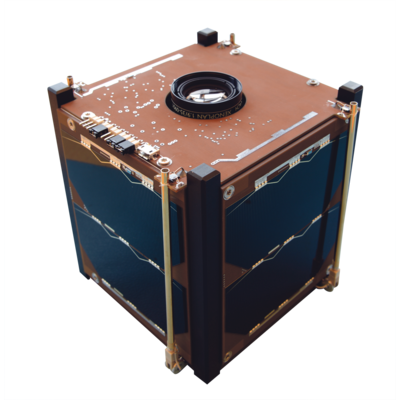
\includegraphics[scale=0.5]{nanoeye}
\caption{GomSpace NanoEye 1U. Courtesy of GomSpace A/S. \cite{gomspaceweb}}
\label{nanoeye}
\end{figure}
\end{center}
\subsubsection{Subsystems}
The satellite consists of several subsystems. The central subsystem of any satellite is the system with the computer designated as the OBC. In the Suomi100 platform it is known as \textit{NanoMind} and is based on an \textit{Atmel} 32-bit microcontroller \cite{nanomindds}. Another vital system to the satellite is naturally the EPS and it is known as \textit{NanoPower} in the platform \cite{nanopowerds}. The communication system of a satellite is the system responsible for receiving commands from the ground, and is responsible for sending information back to the ground as well. In the platform the communication system is known as \textit{NanoCom} \cite{nanocomds}. \par
Besides these essential systems common to all satellites, we have as payload an optical white light wide angle Earth-observing camera and the radio payload measuring \textit{Medium/High frequencies} (MF/HF). The camera came along with the GomSpace platform and is known as \textit{NanoCam} in their catalogue \cite{nanocamds}. Below the most essential subsystems to the topic of this thesis are described in more detail. 
\\
\\
\textbf{On-Board Computer - Nanomind}\\
The Nanomind A3200 On-Board-Computer shown in Figure \ref{nanomind}, is based on an \textit{Atmel AT32UC3C} model \textit{Microcontroller unit} (MCU), which is a 32-bit \textit{Reduced Instruction Set Computer} (RISC) with advanced power saving features. This system runs the software that is responsible for the majority of operations of the satellite, and it works as a sort of mediator between subsystems and routes communication between them. The software is explained in more detail in the following subsection. \par
The MCU has two \textit{Inter-Integrated Circuit} (I2C) buses and one \textit{Controller Area Network} (CAN) bus for communication with other subsystems. It has also 8  \textit{Analog to Digital Conversion} (ADC) pins, which can also be programmed to work as \textit{General Purpose Input-Output} (GPIO) pins. Nanomind contains a \textit{Synchronous Dynamic Random Access Memory} (SDRAM) with 32 MB of capacity for volatile storage as well. For non-volatile storage, the subsystem has a 128 MB NOR Flash. Below in Figure \ref{nanomindblock} is a block diagram of the OBC. \cite{nanomindds}\\
\\
\begin{figure}[h!]
\centering
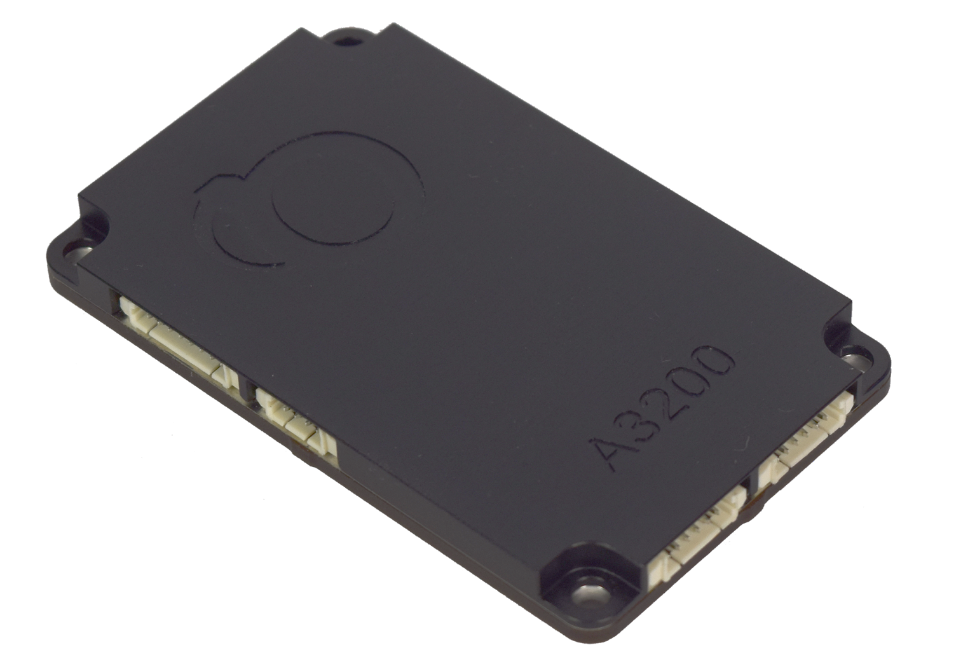
\includegraphics[scale=0.2]{nanomind}
\caption{Nanomind OBC inside its casing. Courtesy of GomSpace A/S. \cite{nanomindds}}
\label{nanomind}
\end{figure}
\begin{figure}[h!]
\centering
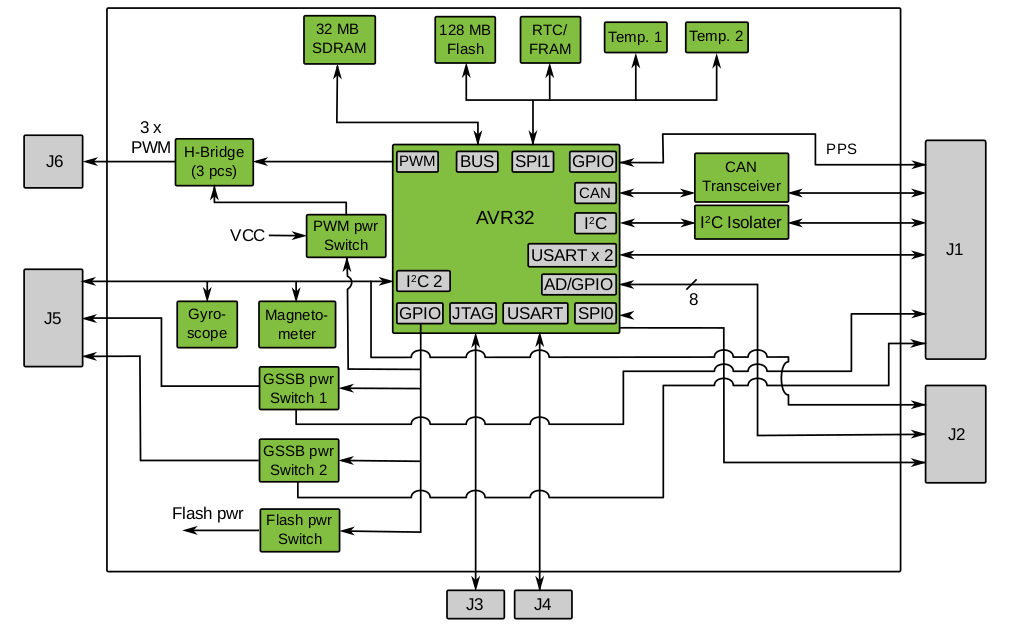
\includegraphics[scale=0.4]{nanomind_block}
\caption{Block diagram of Nanomind. Courtesy of GomSpace A/S. \cite{nanomindds}}
\label{nanomindblock}
\end{figure}
\\
\\
\textbf{Electrical Power System - NanoPower}\\
The Nanopower P31 on Suomi100 satellite contains two lithium-ion batteries and has several reliability features. Figure \ref{nanopower} shows a picture of the subsystem. The batteries are charged by the five solar panels aboard the satellite and the batteries provide power to the whole satellite through the stack connector on the PCB of the EPS subsystem. The system has its own microcontroller, which measures the voltages, currents and temperatures of the system. The microcontroller can also be used to control the 5 V and 3.3 V power buses of the EPS, among other features of the MCU. \cite{nanopowerds}\\
\\
\begin{figure}[h!]
\centering
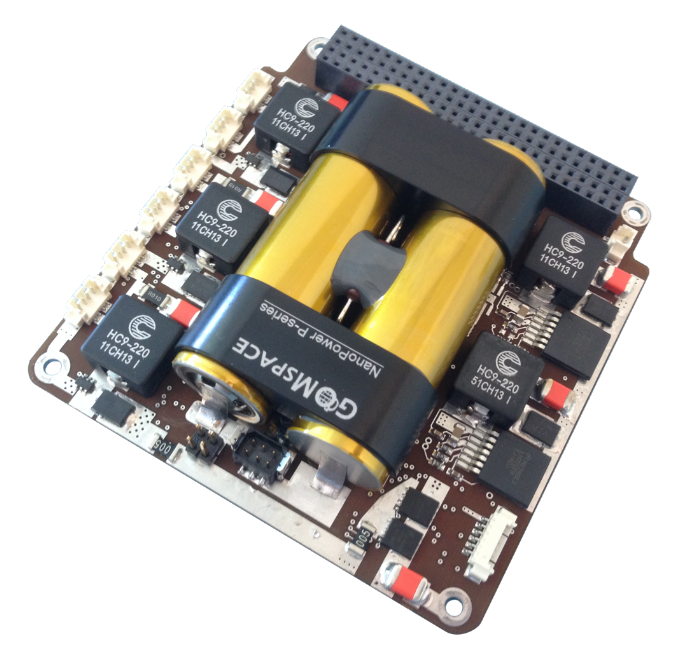
\includegraphics[scale=0.2]{nanopower}
\caption{Nanopower EPS. Courtesy of GomSpace A/S. \cite{nanopowerds}}
\label{nanopower}
\end{figure}
\textbf{Communication subsystem - NanoCom}\\
The NanoCom COM system shown in Figure \ref{nanocom} is a software configurable half-duplex transceiver designed for long-range transmissions. Certain parameters of the system can be      reconfigured on-orbit, such as frequency, bitrate, modulation type and filter-bandwidth. Data rates can be between 0.1 - 115.2 kb/s. The subsystem has its own microcontroller as well as essential radio elements such as \textit{Power Amplifier} (PA) and \textit{Low-noise amplifier} (LNA). \cite{nanocomds}\\
\\ 
\begin{figure}[h!]
\centering
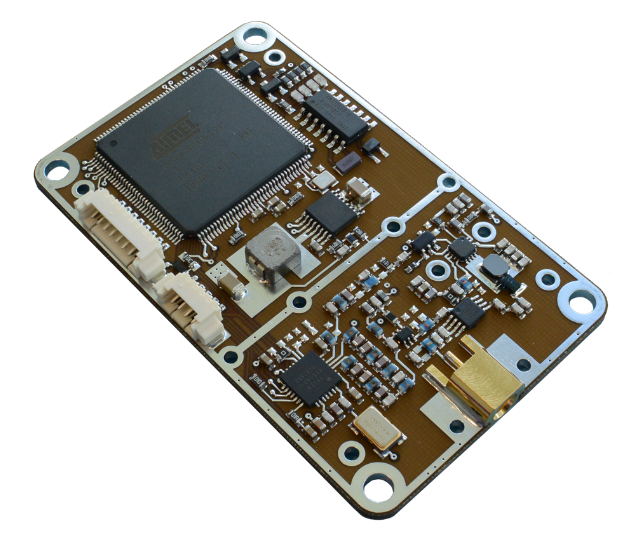
\includegraphics[scale=0.2]{nanocomm_pcb}
\caption{NanoCom communication system. Courtesy of GomSpace A/S. \cite{nanocomds}}
\label{nanocom}
\end{figure} 
\textbf{Camera payload - NanoCam}\\
\begin{figure}[h!]
\centering
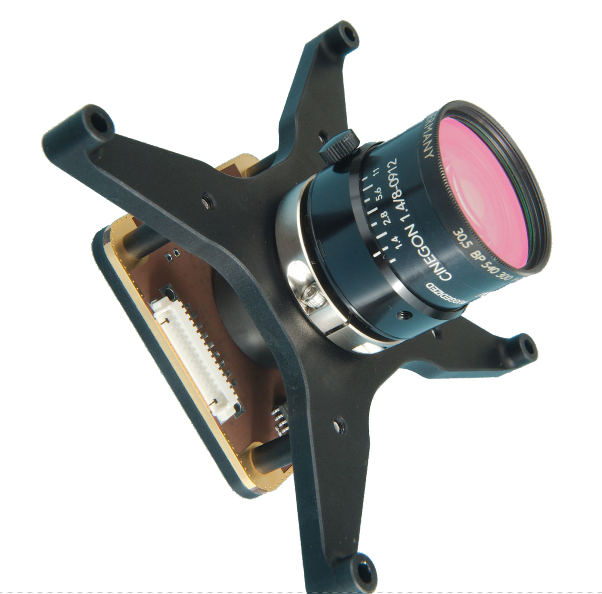
\includegraphics[scale=0.2]{nanocam}
\caption{NanoCam payload camera. Courtesy of GomSpace A/S. \cite{nanocamds}}
\label{nanocam}
\end{figure} 
First of the payloads in Suomi100 satellite is the NanoCam wide-angle white light camera, presented in Figure \ref{nanocam}. The subsystem consists of a lens, image acquisition and processing board. The lens is an industrial grade lens and the image acquisition element is an \textit{Aptina MT9T031} 3-megapixel \textit{Complementary Metal Oxide Semiconductor} (CMOS) color sensor. The processing element consists of a PCB with components such as an \textit{Atmel SAMA5D35} processor with a clock rate of 536 MHz, 512 MB of DDR2 memory for image storing and processing, and a 4 GB eMMC flash drive with 2 GB for image storing. \cite{nanocamds}\par
The software for image processing and storing runs on a customized embedded \textit{Linux} (GomSpace Linux) operating system, and there are several features for image acquisition and storing. The images can be stored in either \textit{RAW, BMP} or \textit{JPEG} formats. Several parameters of the camera system can be altered while in orbit, such as exposure time, different gain values, gamma correction and so forth. \cite{nanocamds}
\\
\\ 
\textbf{Radio payload}\\
The second payload of Suomi100 satellite is the AM radio payload. As noted, this payload was developed by the Suomi100 satellite team, namely by M.Sc Petri Koskimaa, B.Sc Amin Modabberian and B.Sc Arno Alho, based on the concept of the ground-based lightning detector envisioned by Ph.D. Jakke S. Mäkelä \cite{jakke1, jakke2, jakke3, jakke4}. Figure \ref{radiopayload} shows the PCB of this subsystem. Central to the system is the \textit{Silicon Labs Si4740} automotive \textit{Amplitude Modulated/Frequency Modulated} (AM/FM) Radio receiver on an \textit{Integrated Circuit} (IC) \cite{siinfo}. It can receive signals with frequencies from 149 kHz to 23 MHz in 1 kHz steps. The Si4740 can be set to receive AM, AM/SW/LW or FM signals. Several features of the IC can be modified. These include frequency, volume, output format, sample rate, attack rate, release rate and many more. 
Commands to the Si4740 are sent via the I2C bus and the output of the receiver is read via the SPI bus \cite{sids}. \par  
\begin{figure}[h!]
\centering
\includegraphics[scale=0.3]{payload_pcb}
\caption{Second payload of Suomi100, AM radio instrument. Courtesy of Aalto University.}
\label{radiopayload}
\end{figure}
Another important element of this subsystem are the antennas and their support structure. The antennas were designed by M.Sc Petri Koskimaa. Design and construction of the antennas are described in his Master's thesis, "Ferrite Rod Antenna in a Nanosatellite
Medium and High Frequency Radio" \cite{petridippa}. These antennas are four ferrite rods, with two on either side of the support structure forming one antenna. The first antenna is used when listening to frequencies below 2 MHz, and the second one is for frequencies between 1.0 and 9.3 MHz.\par 
The support structure for the antennas was developed by Ph.D Antti Kestilä and it was made with a 3D printer using \textit{Ultem} plastic, a material that can sustain the extreme environment in space relatively well \cite{ultem}.\par 
%\begin{figure}[h!]
%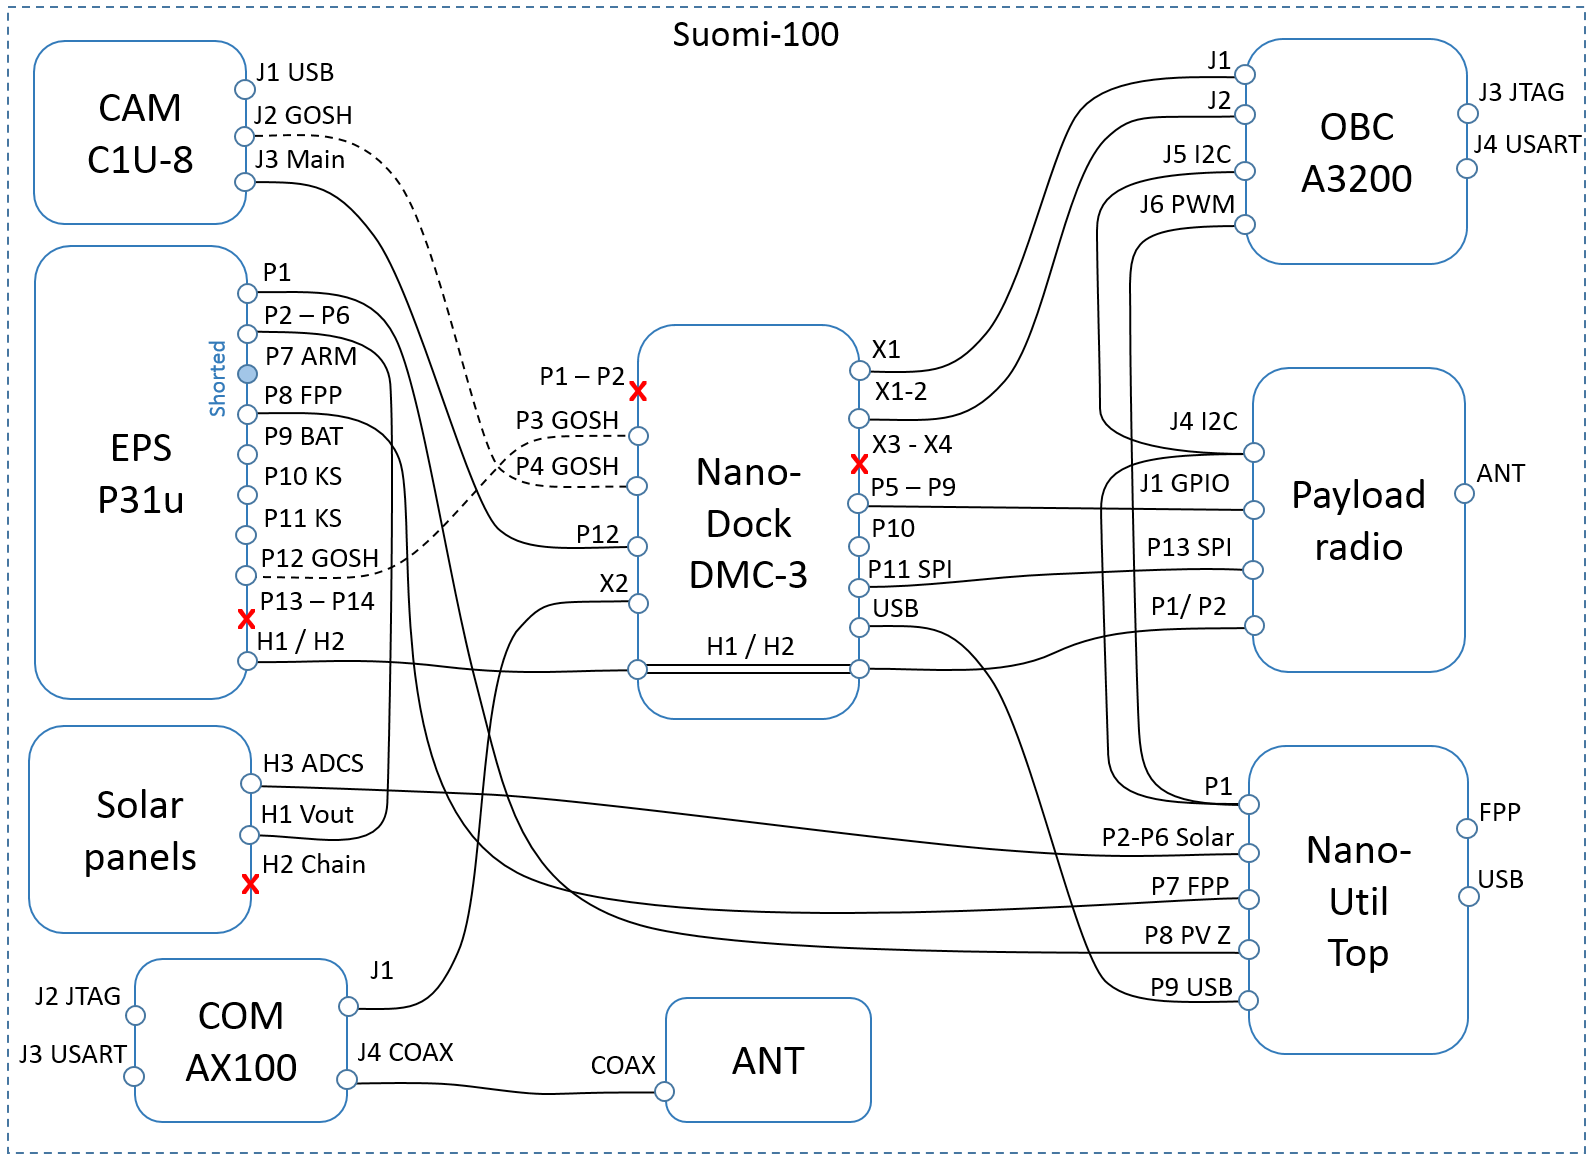
\includegraphics[scale=0.23]{E_interfaces}
%\caption{Diagram of Suomi100 subsystems and their electrical interfaces. Courtesy of Arno %Alho.}
%\label{einterfaces}
%\end{figure}
\subsubsection{Gomspace software}
Besides the subsystems for the NanoEye platform, GomSpace also provided software for all these subsystems. The essential core of the software architecture is a delivery protocol known as the \textit{CubeSat Space Protocol} (CSP), which was originally developed in 2008 by a group of students from \textit{Aalborg University} in Denmark. The protocol has further been developed and maintained by GomSpace itself. In practice, the protocol is used for communication between different subsystems as well as with the ground station. Different subsystems are considered as different CSP nodes in the CSP network. \cite{gomspacesdk}\par 
The protocol as well as the software for the subsystems were written in \textit{C} programming language. In addition to the specific software for each subsystem, all the systems share a set of common functionalities. These common functionalities include sending and storing of HK data, parameter tables for adjusting the different functionalities of a given subsystem, logging functions and inter-subsystem communication through CSP. In addition, each subsystem provides a terminal shell known as GomSpace Shell or \textit{GOSH} for control of the subsystem via a PC by using the \textit{Minicom} software. \cite{gomspacesdk} \par 
The software developed by GomSpace for NanoEye additionally includes such general functionalities as the \textit{File Transfer Protocol} (FTP) running over CSP, with which files and data can be uploaded and downloaded from the satellite. Certain basic file handling routines can be handled with the FTP as well. Among the file handling functionalities is the ability to compress or decompress files with the \textit{ZIP} format. Additionally, the software in the satellite can be updated via the FTP by uploading a software image to the satellite and telling the computer to start reading from it after next reboot. In addition to these, the \textit{Flight Planner} is another general feature of the platform and with it commands can be set to execute at certain points in time either once or repeately with some interval. \cite{gomspacesdk}\par
The operating system running in the NanoMind OBC is a free \textit{Real-time Operating System} (RTOS) known as \textit{FreeRTOS}, which is a lightweight operating system designed for embedded systems that use microcontrollers and small microproserssors \cite{freertosref}. It was developed by \textit{Real Time Engineers Ltd.} in USA. The version of the operating system used in the Suomi100 satellite is 8.0. The operating system is mostly written in C programming language, but certain necessary parts are written with the \textit{Assembly} programming language.\par 
FreeRTOS is a real-time scheduler where different tasks execute in a \textit{Round Robin} fashion, where each task is given some priority value, and tasks with higher priority value are given more processing time. Those with the same priority value take turns in the execution of instructions. Only one task at a time can be in a running state and all the others wait for their turn according to the scheduling policy. In addition to scheduling, the operating system offers functionalities for inter-task communication via \textit{semaphores}, for example. \cite{freertosref}\par 

\subsubsection{Satellite control software - CSP Client}
The ground station software used to control the satellite is known as the \textit{CSP Client}, which is a simple console program for remotely sending commands to the satellite via CSP, a program written by GomSpace in C programming language. The syntax of the software is almost identical to the Gomspace Shell found in the subsystems manufactured by GomSpace. As the source code is available to us, we were able to add our own commands to control the radio payload among other things. In Figure \ref{cspclient} the CSP client is shown running in \textit{Debian 9} Linux, showing among other commands a command inquiring for housekeeping data from the EPS subsystem.\par 
\begin{figure}[h!]
\centering
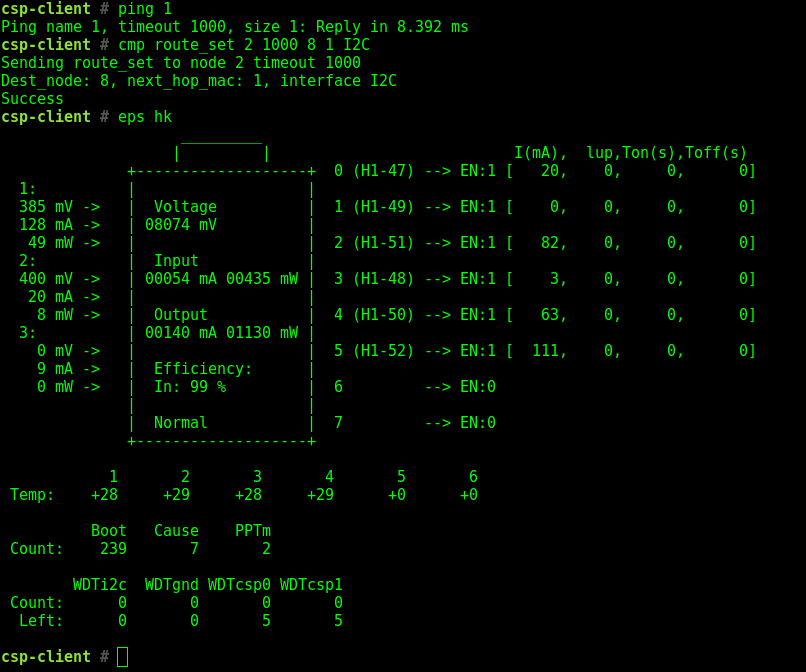
\includegraphics[scale=0.3]{cspclient1}
\caption{Suomi100 ground station control software running in Linux.}
\label{cspclient}
\end{figure}
The software has over a hundred commands if the subcommands related to the main commands are counted. Thus only the main commands used in test automation of Suomi100 are presented here:\\
\\
\textit{\textbf{reboot <CSP node>}}\\
Reboots a CSP node.\\
\textit{\textbf{shutdown <CSP node>}}\\
Shutdowns a CSP node.\\
\textit{\textbf{cmp route\_set <node> <timeout> <addr> <mac> <ifstr>}}\\
Defines a routing path within the CSP network.\\
\textit{\textbf{rdpopt <window size> <conn timeout> <packet timeout> <delayed ACKs> <ACK timeout> <ACK delay count>}}\\
Configures parameters for CSP packet transmissions over radio link.\\
\textit{\textbf{hk get <type> <interval> <count> <t0> <path>}}\\
Get housekeeping data of certain type. Can be received periodically and the data can be stored in the satellite as well.\\
\textit{\textbf{eps hk}}\\
Get housekeeping data from the EPS.\\ 
\textit{\textbf{ping <CSP node> <timeout>}}\\
Test reachability of a certain CSP node within the CSP network.\\
\textit{\textbf{rparam download <CSP node> <mem>}}\\
Download configuration parameters from a CSP node.\\ 
\textit{\textbf{rparam set <name> <value>}}\\
Set configuration parameter value.\\ 
\textit{\textbf{rparam get <name>}}\\
Get the value of a configuration parameter.\\ 
\textit{\textbf{rparam send}}\\
Send the defined parameters back to the satellite.\\
\textit{\textbf{fp server <node> <port>}}\\
Sets the flight planner server to a defined CSP node.\\
\textit{\textbf{fp create <name> [+]<sec> <command> [repeat] [state]}}\\
Creates a flight plan with a defined name and command.\\
\textit{\textbf{cam snap [-a][-d <delay>][-h <color>][-i][-n <count>][-r][-s][-t][-x]}}\\
Takes a picture with the camera on the NanoEye platform. Several features can be defined on or off, such as automatic gain, image thumbnail and so forth.\\

\subsubsection{Software for radio payload}
The software for controlling the AM radio instrument was developed by B.Sc Juha-Matti Lukkari, the author of this thesis, and by M.Sc Jouni Rynö from the \textit{Finnish Meteorological Institution}. Unlike most of the subsystems in Suomi100, the radio payload has no microcontroller of its own or any other general purpose computer. Therefore, the control software operates as a few FreeRTOS tasks in the NanoMind. In addition, new commands for operating the payload instrument were added to the CSP client as well as to the NanoMind GOSH terminal.  \par
One of the radio payload FreeRTOS tasks receives a command as a CSP packet, which is then parsed as a command to be sent via the I2C bus on NanoMind to the Si4740 IC, for example. Command of the Si4740 is based on the hexadecimal values of the bytes it receives \cite{sids}. The first byte received defines which action is being performed and the following bytes define the arguments for that respective action \cite{sids}. The IC then gives a response byte, with hexadecimals 80 and 81 implying a succesful command, and ,for example, 40 or 0 implying a failed command \cite{sids}. \par
Over 50 different arguments for different commands can be used when controlling the Si4740 \cite{sids}. Therefore, when commanding the radio payload to perform a measurement, the different values for different arguments are loaded either from a configuration file or from a GomSpace paramater table. The parameter table and the configuration file were separately added to the NanoMind. All the commands can choose to use either one of these argument sources. In addition, the commands can be used "manually" without loading any external configuration for the command. \par
Some of the most essential commands for the radio payload operation in CSP client are presented here:
\\
\\
\textit{\textbf{radio on <config> <reg>}}\\
Turns on the Si4740 chip, among various other operations needed to setup the payload.\\
\textit{\textbf{radio operation <config> <config> <mode> <mode arguments>}}\\
Runs one of the radio operation modes defined in section 2.5.3.\\ 
\textit{\textbf{radio set\_property <config> <property> <value>}}\\
Sets one property of the Si4740 to a defined value.\\
\textit{\textbf{radio get\_property <property>}}\\
Gets the value of a certain property defined in the Si4740.\\
\subsection{Automating testing of Suomi100}
One of the \textit{research purpose and goals} pointed in section 1.4 was the aim of using test automation to perform testing for the Suomi100 satellite, and Robot Framework was defined as the test automation framework for this task. The detailed technical solution for automating the testing of Suomi100 is described in this section.
\subsubsection{API and communication layers for CSP Client software}
In order to automate the control of the satellite, some form of interface is needed which can
communicate between the satellite and the framework used to perform the tests.
Fortunately, the Gomspace software already provides a terminal shell program called \textit{GOSH} on each of the subsystems \cite{nanomindds}. In addition, all of the subsystems can be controlled from a single shell via a serial to a \textit{USB FTDI} cable connected to \textit{NanoUtil} USB port \cite{avrtoolchain}. As presented in the previous subsection,  a separate CSP client
software tool exists, which can be used to control the satellite from the 
ground station via a radio link, and it can also be used to control the satellite via the FTDI cable.\par
Automating the control of the CSP client software was chosen as the solution on how to 
automate the control of the satellite. The CSP client was chosen, because by automating
control of it, we can perform tests via the radio link as well. The automation was first done by
modifying the source code of the \textit{main.c} file of the CSP client, which contains the C-language main function for the program. The modification consists of creating a \textit{POSIX thread} which runs a function that opens and listens to a socket connection on the \textit{localhost} local network address. The localhost is a specific network address referring to the computer itself \cite{linuxproginterface}. When a message is received on the opened socket, the thread then runs the command on the CSP client terminal, as if a user would have written the command on the terminal. Alternative solutions could have been used, for example a separate program could have been written and the CSP client could have communicated with it through some of the inter-process communication methods provided by the Linux operating system. This could have been made through Linux output and input \textit{standard stream} redirection methods such as \textit{pipes} \cite{linuxproginterface}. Using the network connection, however gives the potential to make the automation externally controllable. \par 
Over the course of development of the libraries and test suites, a more direct approach of using the \textit{standard input stream} (stdin), to send commands to the CSP client was also chosen. Furthermore, an even more direct method of simply automating the keypresses of the keyboard was implemented with the aid of a Python library called \textit{pyautogui}. The benefit of having the communication performed with stdin or with automated keypressing through a Linux \textit{kernel} keyboard driver, is that we can automate the use of not just the CSP client but the use of many different terminal programs. Even programs with source codes that we have no access to, thus omitting the need to write a separate \textit{Application Programming Interface} (API) into them as was done with Suomi100. Nonetheless, using self-tailored process communication APIs which work via e.g. pipes or sockets, have some advantages over these sort of "crude" methods. For example, use of stdin can be reserved to the program in a way that it is not accesible outside the program itself. Sending the commands by automating keypresses can bypass this. However, if a user uses the computer during testing, the keypresses can be received by programs that we did not wish to automate.\par
Nonetheless, in order to create a generic test automation library, all of these process communication methods are incorporated into the release version of the CubeSat test automation function library, which is explained in more detail in section 4.
If we ourselves write the terminal software with our own testing library in mind, all of these communication methods should be valid for automating the testing.  \par 
Besides requiring the method of sending commands to the satellite to be performed in an automated fashion, we also must know how the satellite responds to these commands in order to verify the tests as either passed or failed. The CSP client software fortunately receives responds to the commands sent to the satellite, and thus we have some knowledge of how the satellite behaved. It was found that the easiest solution would be to read the \textit{standard output stream} (stdout) of the CSP client program and transfer the responds to the verification functions in the function library.\par
Another way for the capture of the responses to the commands would be to modify the source code of the CSP client for it to send the received outputs of the executed commands to another port on the socket connection. In this way we could then listen to this port on the function library. Doing the transmission of CSP client output to the test automation libraries this way was experimented by using some Linux output redirection routines such as \textit{dup} \cite{linuxproginterface}. However, there were some difficulties with the implementation, and due to time constraints it was easier to monitor the standard output of the client software. Furthermore as mentioned before, during the development of the test automation libraries, use of stdin for communication was developed as well. In fact, as with using stdin to send commands to the process, reading the stdout of the process allows us to create a generic test verification solution to this as well, provided that the process which we wish to perform automated tests on responds through the stdout stream, which fortunately happens to be the case for most terminal programs \cite{linuxproginterface}.
\par   
The solution for the communication is illustrated in Figure \ref{cspauto} and the modified \textit{main.c} for the CSP client can be found in Appendix \ref{LiiteD}.
\begin{figure}[h!]
\centering
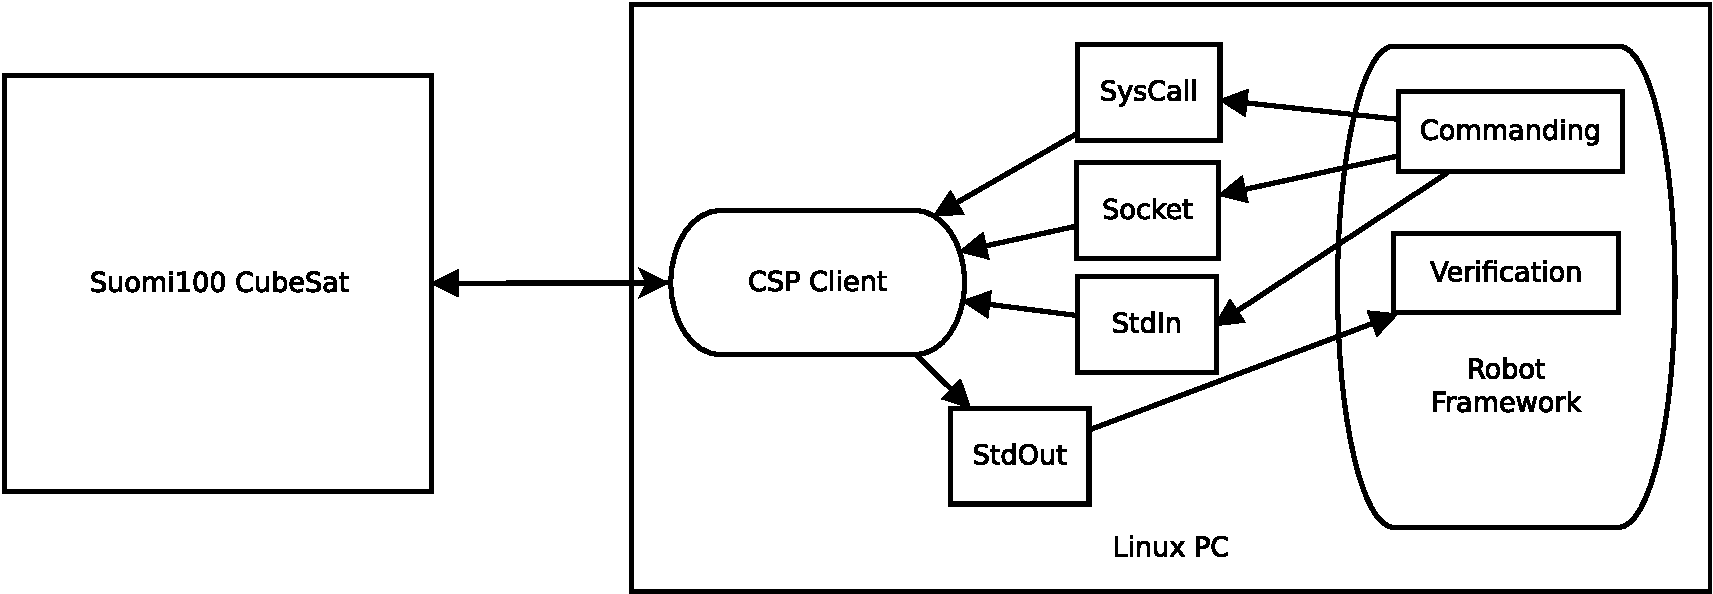
\includegraphics[scale=0.5]{cspautomation}
\caption{Illustration of the software architecture developed for Suomi100 test automation. Large rectangles represent environments, small ones represent layers and rounded rectangles represent programs.}
\label{cspauto}
\end{figure} 
\subsubsection{Python libraries}
A set of function libraries using Python programming language were written. All of these libraries each consisted of one Python class. The class of the core library, known as \textit{CubeSatAutomation}, has the methods for the communication with the CSP client via any of the three methods, socket, stdin or automated keypressing via the pyautogui library. Furthermore, the library includes the methods to read and verify the process replies from stdout.
As can be seen in Figure \ref{cspauto}, the commands are sent to the CSP client through any of the three communication routes and the output of the program goes to the stdout. The output is then caught and read by the CubeSatAutomation library and test cases and test steps or keywords are failed or passed based on the output read from the CSP client. \par
It is importation to note the following details about the test automation libraries. 
\\
\\
\textbf{CubeSatAutomation library}\\
CubeSatAutomation library has the crucial functions for sending commands, opening socket connection, opening and closing the opened program and others. Besides being able to open the CSP client program, any program can be automatically opened with the library as the method for opening uses the standard Python \textit{subprocess} library. All the other libraries implemented use the core methods in CubeSatAutomation, for example, to send commands to the CSP client to execute. These other libraries have subsystem-specific functions for the test automation. To create only one open communication route between the CSP client and Robot Framework and to have only one handle on the CSP client program process, the core library defines these as \textit{class variables}, which are then accessed by the subsystem libraries. In practice this means that we do not open several CSP client programs and several connection routes separately for each subsystem library included in the test suite. Instead, the program and the communication route is opened only once for each test suite.\par 
Another class variable which defines the scope of the instance of the class in the Robot Framework was defined as well. This was set to define the scope of the library to be on the suite level. By having the scope on the suite level, only one instance of the library class is declared per test suite, thus again having only one handle on the client software and having only one connection route open during the execution of a test suite \cite{robotuserguide}.\par 
The essential core methods used in the CubeSatAutomation Python class are presented below in the form of Robot Framework keywords:
\\
\\
%\textbf{client_start(self, config_file=None, prog=None, params=None)}
\textit{\textbf{Client Start  <config file> <program> <parameters>}}\\
Start the program that is to be automated (CSP client). In addition, command line parameters as well as some additional configurations can be defined.\\
\textit{\textbf{Client Close <socket> <program>}}\\
Close the program and the possible socket assiocated with it.\\
\textit{\textbf{Connect Socket <config file> <server> <port>}}\\
Opens a socket connection to a defined server and port address. These values can be read from a configuration file as well.\\
\textit{\textbf{Send Command  <message> <option> <timeout> <read timeout>}}\\
Sends a command through the socket connection and reads a reply from the standard output. The reply can be stored temporarily or discarded.\\
\textit{\textbf{Write Command  <message> <option> <timeout> <read timeout>}}\\
Writes a command to the standard input and reads a reply from the standard output. The reply can be stored temporarily or discarded.\\
\textit{\textbf{Type Command  <message> <option> <timeout> <read timeout>}}\\
Types a command by automating keypresses on the keyboard and reads a reply from the standard output. The reply can be stored temporarily or discarded. \\
\textit{\textbf{Persistent Command  <message> <exception replies> <end reply> <timeout> <read timeout>}}\\
Writes a command persistently to the standard output until a defined reply is read or either a specific error reply is read or a timeout value is reached.\\
\textit{\textbf{Verify Reply Contains  <message> <timeout> <read timeout>}}\\
Reads several lines from the standard output and tries to find for a defined message from the lines.\\
\textit{\textbf{Verify Reply Contains Not  <message> <timeout> <read timeout>}}\\
Reads several lines from the standard output and tries not to find for a defined message from the lines.\\
\textit{\textbf{Verify Reply Contained  <message> <timeout> <read timeout>}}\\
Tries to find a defined message from the replies that were stored by an earlier command.\\
\textit{\textbf{Wait Until Reply Contains  <message> <timeout> <read timeout>}}\\
Reads from the standard output until a defined message is found or a timeout is reached.\\
\\
Finally, here are some of the keywords presented that are specific to GomSpace NanoEye.\\
\textit{\textbf{Set Satellite Parameter  <device> <parameter> <value>}}\\
Sets value of a configuration parameter of a defined device in the CSP network. \\
\textit{\textbf{Send Satellite Parameters}}\\
Sends the set parameters back to the satellite.\\
\\
\\
Creation of a skeleton core library is the aim of the final development of the test automation library. This library only has the aforementioned methods to start and communicate with a desired Linux program running on a terminal shell and keywords that are more specific to the Suomi100 or CSP client are omitted. With the aid of this library, satellite software developers wishing to automate testing of their satellite and satellite software, can       create their own specific libraries suited to their own needs. The final version of the CubeSat test automation library is described in section 4.\\
\\
\textbf{Subsystem libraries}\\ 
Other libraries developed for test automation of Suomi100 are called \textit{NanoCam.py} and \textit{RadioPayload.py} and these are intended for the automated testing of NanoCam and radio payload subsystems respectively. The classes of both of these create an instance of CubeSatAutomation class, instead of calling for specific functions or methods of that class from the outside. By doing this, the class variables including handle to the automated process, socket address and others are passed to all these other classes as well. The methods of these classes thus use the methods of CubeSatAutomation directly.\par
The specific methods defined by the NanoCam test automation library are presented below as Robot Framework keywords:\\
\textit{\textbf{Camera Startup	<timeout>}}\\
Reboots the camera and downloads parameter Table 1 from the subsystem. Timeout specifies the time that we wait for the camera subsystem to come online in satellite bus.\\
\textit{\textbf{Camera Take Picture	<timeout> <store format> <filename> <autogain>}}\\
Sets image format and filename in the camera and takes a picture with the given autogain value (empty at default). Keyword fails if the image is too dark (less 5 \% light) or too bright (over 95 \% light).\\
\textit{\textbf{Camera Load Picture	<stored file> <loaded file>}}\\
Downloads the file stored in NanoCam to the PC running the CSP client program.\\
\\
The subsystem specific keywords for the radio payload are defined as the following:\\
\\
\textit{\textbf{Radio Startup  <switch input> <switch power> <antenna input>}}\\
Sets up and starts the radio payload. The antenna and switch to be used can be additionally defined.\\
\textit{\textbf{Radio Powerdown}}\\
Turns off the radio payload.\\
\textit{\textbf{Verify Radio Status}}\\
Checks for the status of the Si4740 chip.\\
\textit{\textbf{Run Radio Mode  <parameter file> <property file> <mode> <mode arguments}}\\
Runs one of the radio operation modes defined in section 2.5.3.\\
\textit{\textbf{Verify Radio Results  <buffer file> <timeout>}}\\
After the operation mode is completed, inspects the outputs that the payload sent and fails if certain outputs contained errors tied to the operation of the Si4740 chip. \\
\textit{\textbf{Radio Load Data  <stored file> <loaded file> <timeout>}}\\
Downloads a measurement done by the radio payload.\\
\textit{\textbf{Radio Plot Data  <file> <output file> <plot image>}}\\
Draws a graph from downloaded radio measurement data.\\
  
    
\subsubsection{Robot framework test suites}
The test cases follow the keyword-driven approach and the keywords are written to be short and mostly to be non-specific to the test case. The functions and methods written in Python and described in the previous section are used directly as such. This is because, the approach was to make a smaller set of versatile and generic keywords that could be used over many test cases and test suites. This approach was felt to be more efficient as there would be less need to maintain the test suites if they did not have large set of specific, though descriptive keywords, which is common with Robot Framework. Besides, the Suomi100 satellite project is not a typical software project where stakeholders would go over the test suites and validate them. All people involved in the project have a technical background. In addition, having a set of general keywords that are not entirely tied to Suomi100 is beneficial if some future satellite project wishes to use the testing methods and tools described in this thesis.\par
Each of the test cases are tied to a particular operation mode. The operation modes are discussed in detail in section 2.5. The purpose of each test case is to verify the functionality of some aspect of a particular operation mode. Each test case is marked with the Robot Framework \textit{[Tags]} marker to identify which operation mode the test case is related to.
In addition, each test case begins with a \textbf{\textit{Satellite State}} keyword defining the state of the satellite. For example, one such state is when the satellite has restarted itself. This keyword was written in order to make the test cases independent of each other and to have a degree of reproducability for the tests. In some cases, the test cases need to be dependant on each other and in such cases the satellite is not specifically set to a certain state. Such states are called as \textit{Unknown} and \textit{Communicating}, for example.\par 
The test suites are divided firstly based on the four different larger features that are tested with the Suomi100. Namely, separate sets of test suites are written for camera payload, radio payload, NanoEye basic functionality and for "Day in the life" testing. Each aspect of a feature further divides the test suites into test suites testing different parts of a  particular feature.\par   
\subsection{Test setups and environment simulation}
The different aggregates for testing of the Suomi100 were defined in section 2.4. For simulating the functional environment of the satellite for these different types of tests, four different environments were set up. Two different environments for testing two different payloads (1 \& 2), one for testing basic operational features of the NanoEye platform (3) and one larger environment for the operational scenario testing of the satellite (4). 
\subsubsection{Camera payload testing}
For the testing of the NanoCam and the \textit{imaging operation mode}, we tried to find something facing the camera with similar color and brightness values as what the camera would see while in orbit. The easiest solution would be to simply take the whole integrated satellite outside on a bright day to the balcony on top of the \textit{TUAS} building in Aalto University at Maarintie 8. The satellite stands on top of a stand, and the side with the camera lense is directed towards horizon. A PC with the CSP client and the test automation tools are connected to the satellite via the USB connection on the NanoUtil. In addition, the satellite is loosely enclosed in a plastic container to protect it from particles in the air. 
Figure \ref{camerabalcony} below shows the test setup used during the testing.\par 
\begin{figure}[h!]
\centering
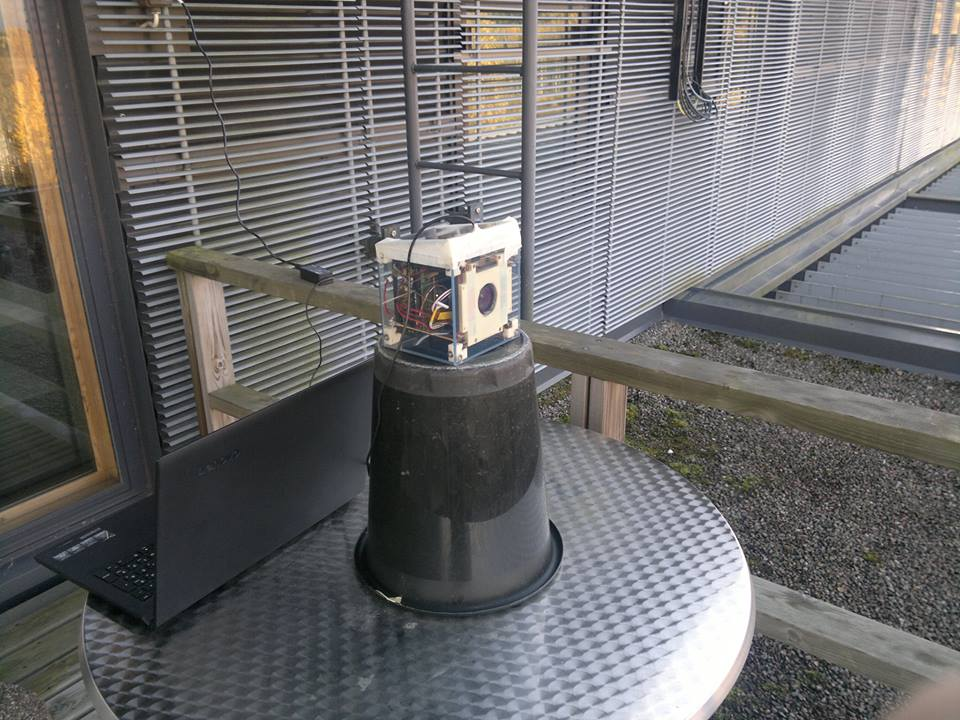
\includegraphics[scale=0.3]{camerabucketspurgu}
\caption{Suomi100 satellite on a balcony during imaging mode tests.}
\label{camerabalcony}
\end{figure} 
\subsubsection{Radio payload testing}
The environment for the testing of the radio payload is set up in the clean room of Aalto University's space laboratory. The satellite is connected via the USB connection to a PC with the CSP client software and the test automation tools. The functional environment is simulated with a radio signal source in order to create some artificial noise in radio frequencies that would mimic the radio signals present in the Ionosphere. The radio noise is generated with a \textit{HackRF One} \textit{Software Defined Radio} (SDR), which is connected to another PC running \textit{GNURadio} signal processing software.
Figure \ref{s100hackrf} shows the setup for the testing of the radio payload.\par   
\begin{figure}[h!]
\centering
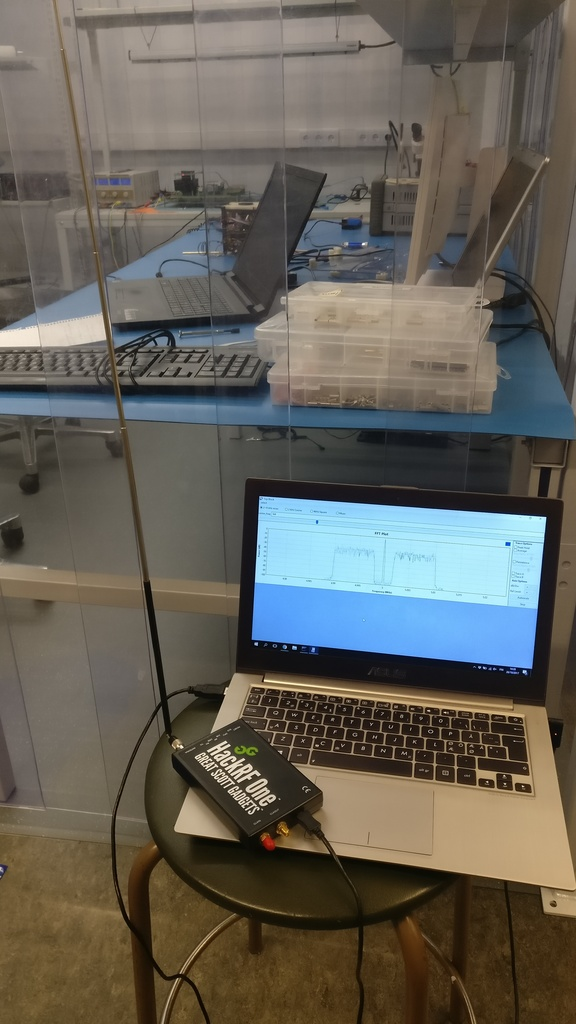
\includegraphics[scale=0.3]{payload_testing_hackrf}
\caption{Radio payload testing with \textit{HackRF One}.}
\label{s100hackrf}
\end{figure}
The frequencies that are used in the environment simulation are 2 MHz, 5 MHz and 9 MHz. These were chosen based on the requirements of the payload (should operate in range of 1-10 MHz) and the limitations of the hardware, as the HackRF is not able to produce signals with frequencies  lower than 2 MHz. Furthermore, the antennas attached to the payload themselves cannot receive signals that are much higher than 9 MHz. The middle frequency was chosen to be 5 MHz based on the research done on the radio signals in the Ionosphere. This frequency would be of most interest to the research conducted by the Suomi100 satellite mission \cite{esanpapru}. 
Figure \ref{gnuradio} shows a \textit{Fast Fourier Transform} (FFT) plot of the noise that is generated from the GNURadio, which is then transformed into radio waves by the HackRF.\par
\begin{figure}[h!]
\centering
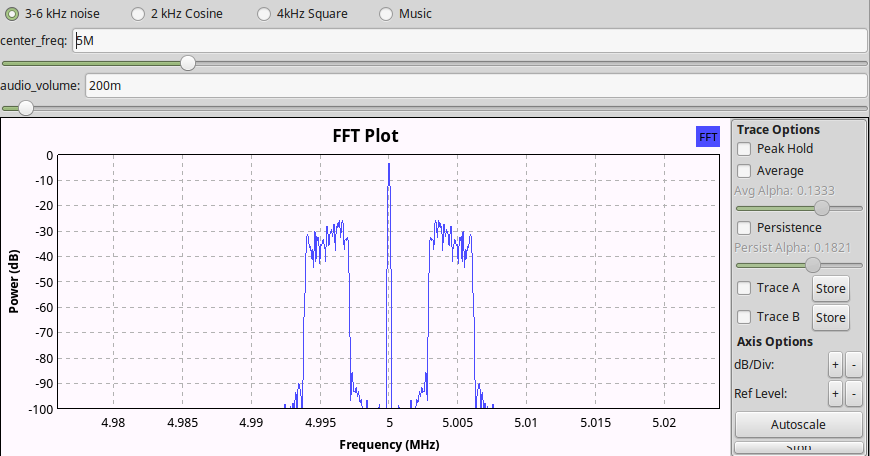
\includegraphics[scale=0.45]{Test_window}
\caption{Screenshot from \textit{GNURadio} signal processing software showing FFT plot of radio noise being generated.}
\label{gnuradio}
\end{figure}  
\subsubsection{Satellite basic operations testing}
For testing of the basic satellite operational features such as collection of housekeeping and safe rebooting during an error, no external inputs to the satellite are used. The satellite is in the clean room of Aalto University's space laboratory connected to a PC with the CSP client. 
In Figure \ref{basictest} we have a picture of this setup.
\begin{figure}[h!]
\centering
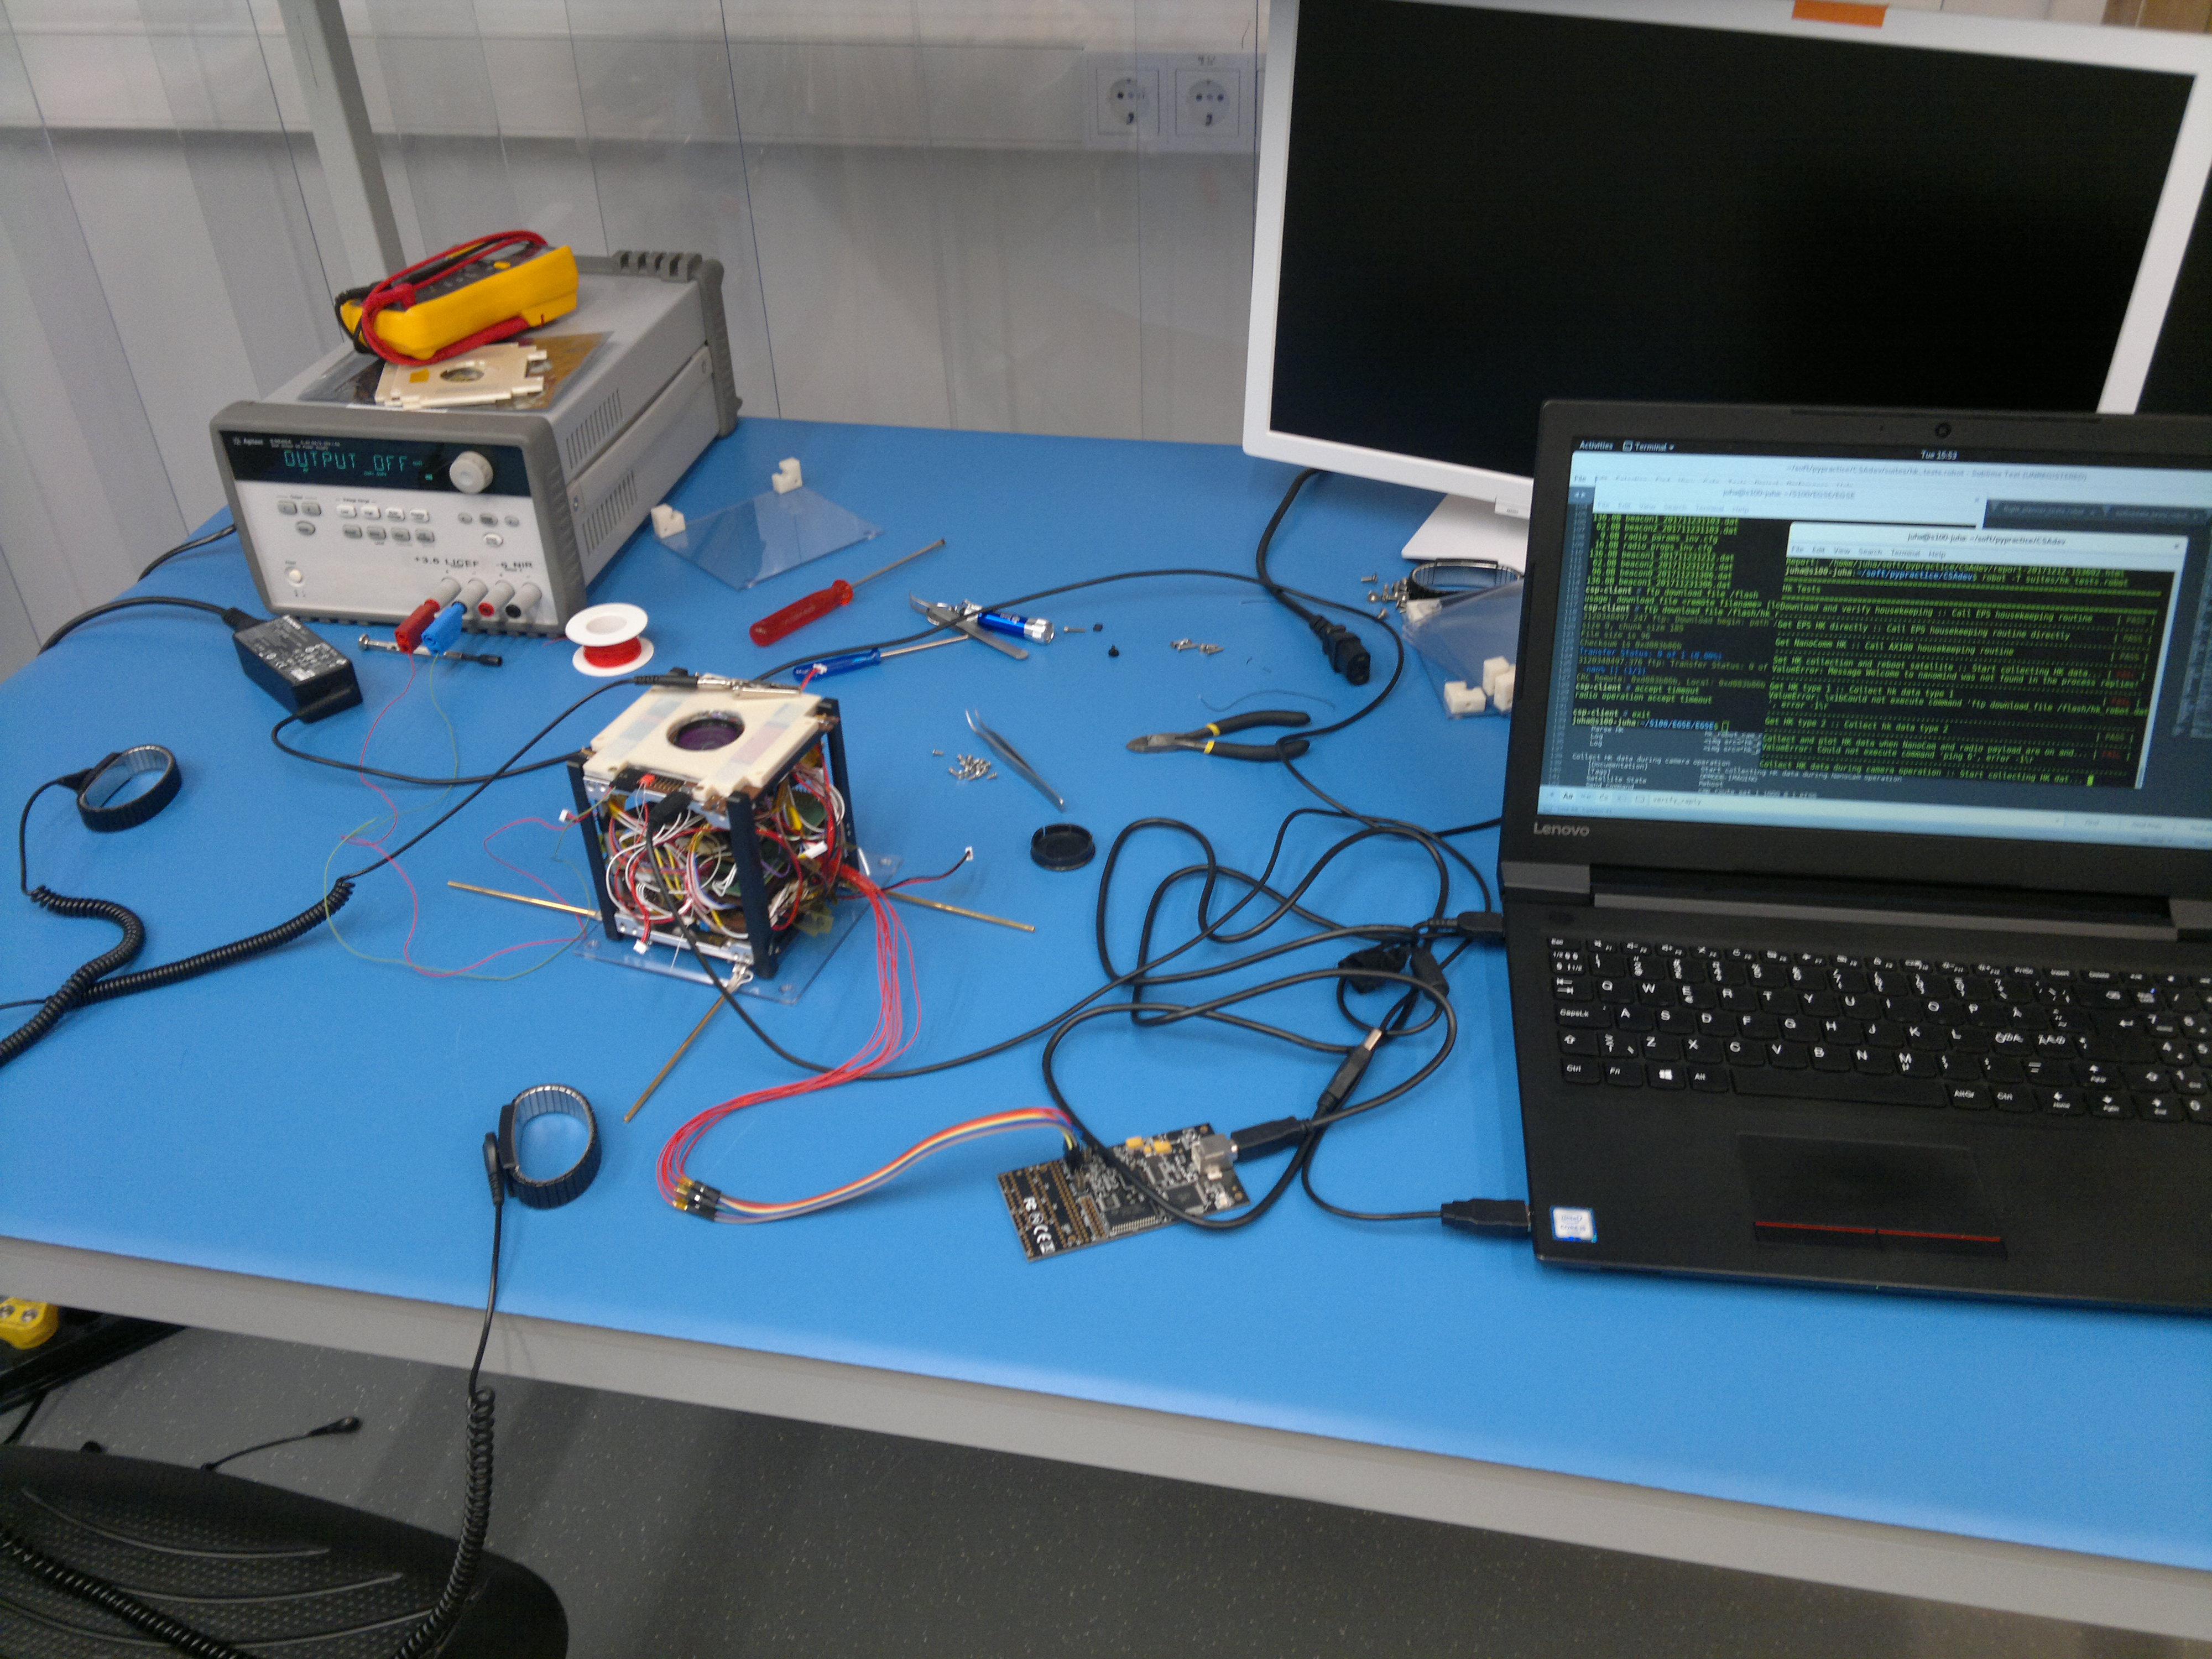
\includegraphics[scale=0.3]{basicsetup}
\caption{Setup for testing of basic functionalities of the NanoEye platform. Suomi100 is on the left and a PC with CSP client, and a PC with the CSP client and the test automation softwares is on the right.}
\label{basictest}
\end{figure}  
\subsubsection{Operational scenario testing, "Day in the life"}
In "Day in the life" operational tests, the Sun is simulated with a %\textit{Philips BMH 1800L 55} 
1800 Watt Xenon lamp that is situationed approximately 1.5 meters away from the satellite. Two solar panels are connected to the satellite in the manner they are connected during flight. The satellite faces the lamp in an angle so that both panels receive light from the lamp. As the lamp is quite powerful, we can really verify that the solar panels charge the batteries in the satellite. In addition, the lamp can heat the objects it is faced towards and this was used as a method to add some thermal features to the test. The idea is to use the lamp for the duration it takes the satellite to heat up to 50 degrees Celcius under the illumination and then let it cool back to room temperature (approx. 27 Celcius in the clean room). The heating and cooling was measured with \textit{FLIR E6} thermal camera and the heating duration was measured to be approximately 10 minutes and the cooling down period was measured to last ca. 20 minutes.\par
In Figure \ref{dayinlife1} this setup with the solar simulator is presented.\par
\begin{figure}[h!]
\centering
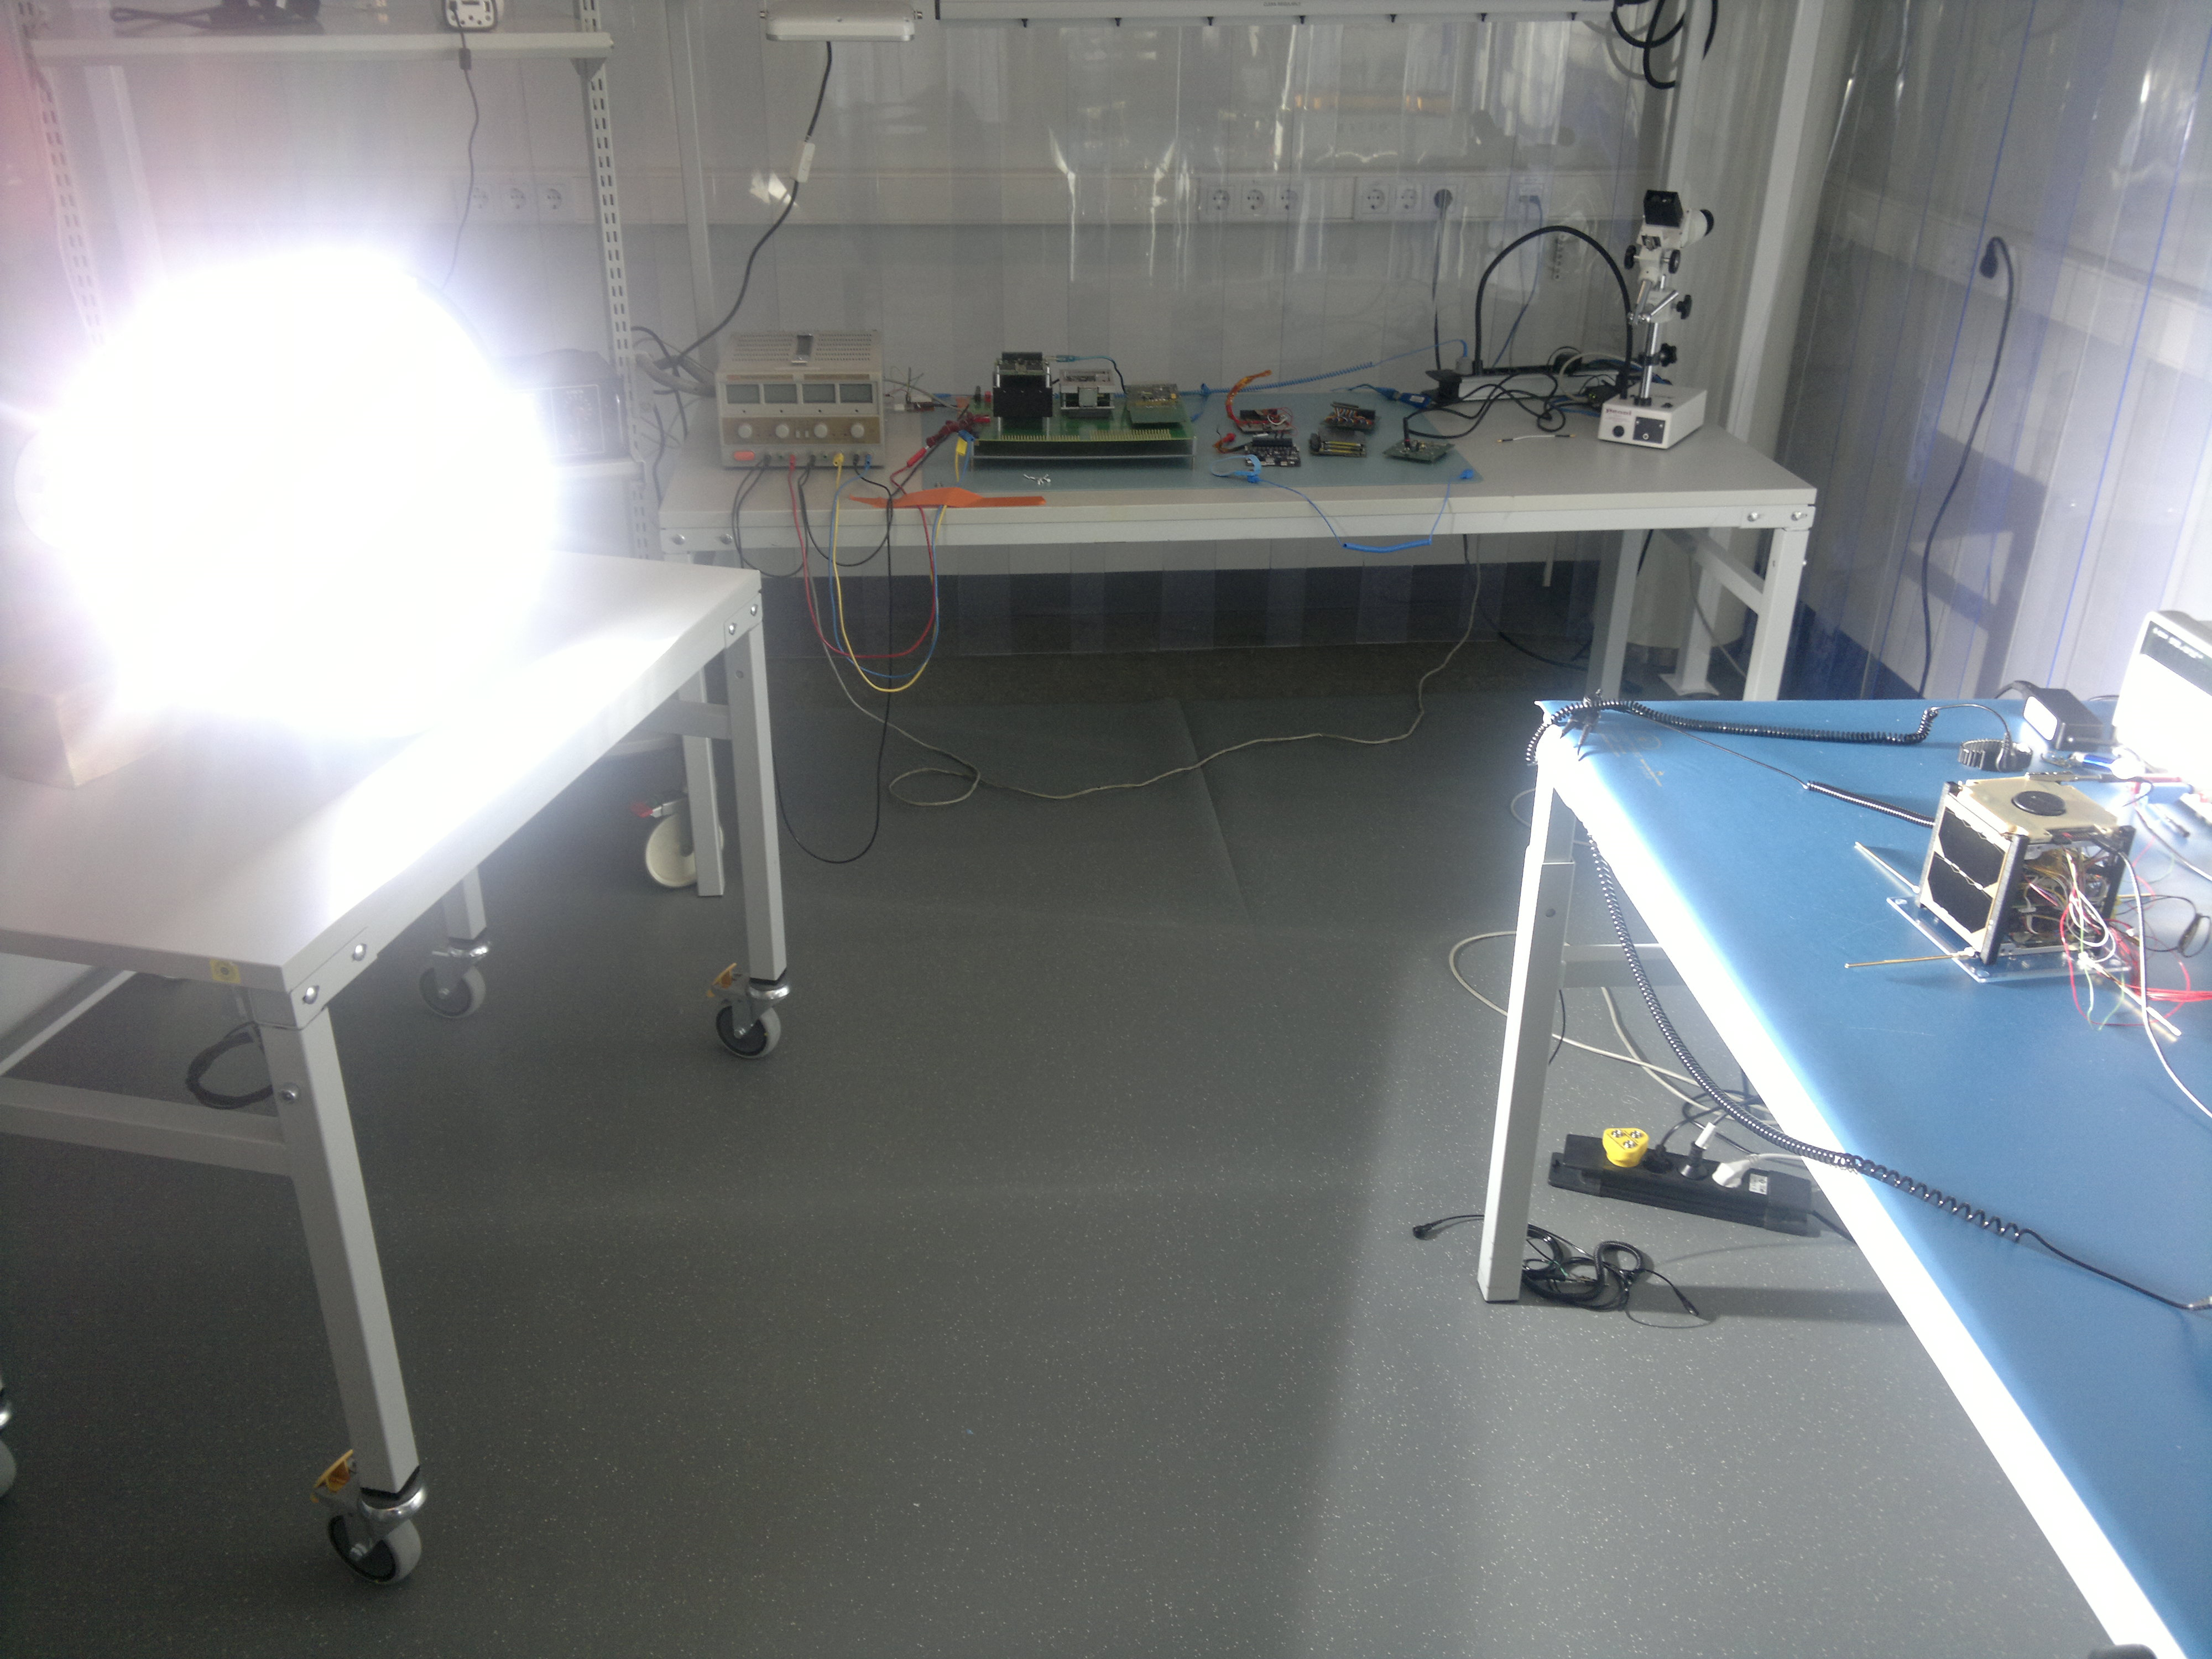
\includegraphics[scale=0.3]{daysetuplamp2}
\caption{Day in the life setup for the satellite. The Xenon lamp is on the left and Suomi100 CubeSat is on the right in the picture.}
\label{dayinlife1}
\end{figure} 
For the "Day in the life" testing, these periods form the phases of the operational scenarios. When we pretend that the satellite comes from eclipse, we turn on the Xenon lamp and we are in communication with the satellite for 10 minutes and after that the lamp is turned off and we pretend that the satellite goes out of the reach of our ground stations and stays there for 20 minutes. In addition, the 10 minutes communication window roughly corresponds to the time that we can be in communication with the satellite during one revolution around Earth by the satellite.\par 
Unlike in the setups described previously, the control of the satellite happens via radio link. A SDR with model \textit{Ettus USRP B200} is connected to a PC with the CSP client software and the test automation softwares. This SDR is the one used in the actual ground station and for this testing the SDR and the PC were located in the next room in Aalto University's space laboratory. The actual groundstation and all of its hardware is not used because the solar simulator has to be controlled manually and the groundstation is situated several floors up from the Aalto University's Space laboratory. Nonetheless, the same software and the same SDR are used as what will be used in the groundstation.\par 
Figure \ref{dayinlifelink} presents this setup.\par
\begin{figure}[h!]
\centering
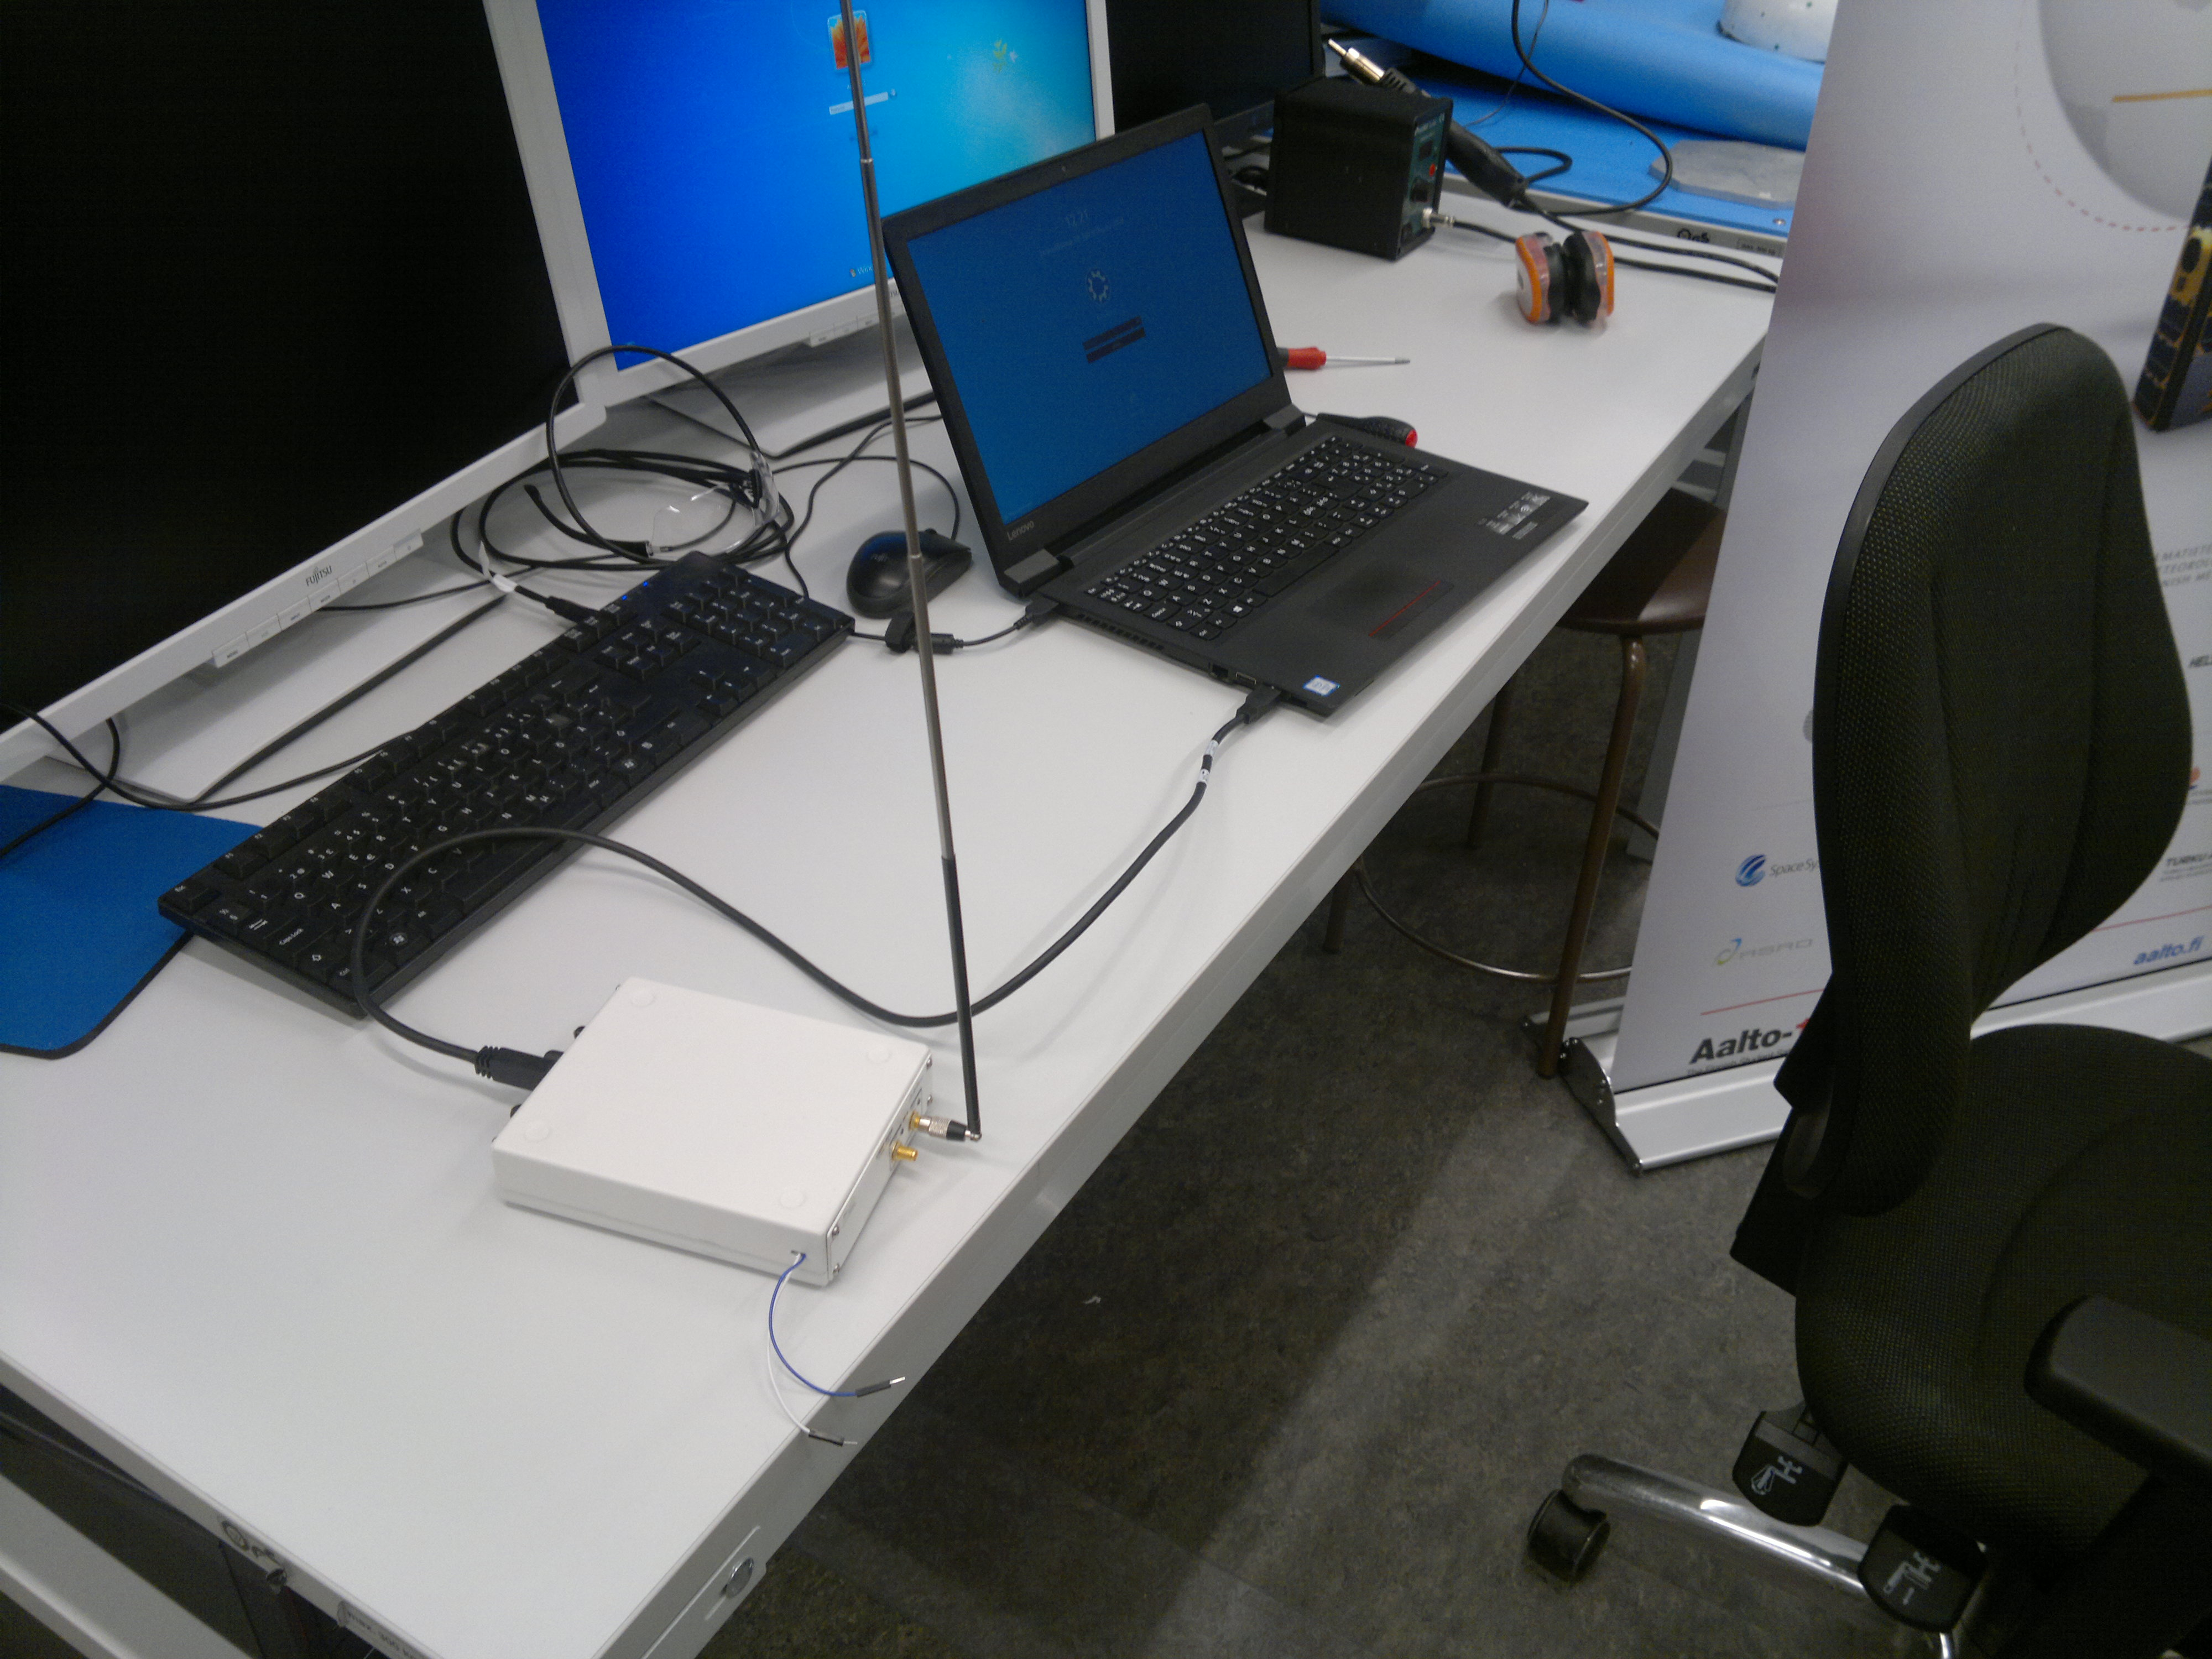
\includegraphics[scale=0.3]{daysetuplink}
\caption{Day in the life setup for a "stripped down" groundstation.}
\label{dayinlifelink}
\end{figure} 
\clearpage
\section{Results and Discussion}
%\section{Tulokset}
\subsection{Executed tests}
The Robot Framework test suites executed can be divided into three categories: test suites done for the two payloads (1), test suites written for general satellite operations (2) and test suites for "Day in the life of the satellite" operational scenario tests (3). \par 
The first category of suites follow the more traditional method of combinatorial testing. Each test case was derived from the operation modes defined for the camera and radio payloads. Each of the test cases for their representative operation mode are identical in steps, but use different combination of values in the keyword arguments. Since the payloads perform only singular functions, it was felt that using combinatorial input values was necessary to have adequate test coverage for these payload operation modes. \par
The second category consists of test suites made for the functional testing of the commands that contribute to the basic operations of the satellite. These test cases for different operations are completely different from each other in design and the tests here begin to resemble different smaller scenarios or use cases. Such cases as telemetry gathering, flight planner commands, software update, etc. In addition, a test suite was written for testing restarts of the subsystems and of the OBC and of the whole satellite as well. The requirements and use cases for the tests were partly derived from the manuals provided by GomSpace, but mostly these tests were informal in nature.\par 
The third category, follows the higher level satellite system integration tests where the satellite is tested based on operational scenarios defined for a "Day in the life of a satellite". Separate test suites were written for each operational scenario. The test cases at this level are simply different phases in the operational scenario.\par
In addition to these test suites, another one was used during the development of the software for the radio payload. This test suite resembles a smoke test and it has limited set of test cases, testing each of the operation modes. Yet, no proper continous integration chain was done during this time, but the smoke tests were manually started usually once every week.\par   
\subsubsection{Camera payload}
The test cases for the NanoCam were identical in structure, or in other words, several test cases were made for the same use case of the camera payload. Only difference was that the main parameters such as gain value and exposure time differed between test cases. These two are the main parameters according to the NanoCam manual provided by GomSpace \cite{nanocamds}. Having the exposure time fixed, combinatorial test input selection was used to go over different combinations of camera parameters. Three different values of the exposure time were used and for each value, the same parameters other than exposure time were changed in different test cases. The values used for the exposure time were 10, 30 and 90 milliseconds.  Below is Figure \ref{robotcamera} showing the test case structure used in testing of the camera payload.\par
%\begin{figure}[h!]
%\centering
%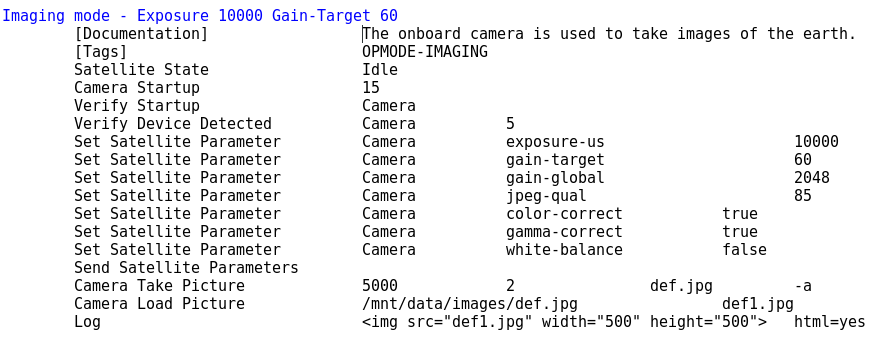
\includegraphics[scale=0.5]{cameracase}
%\caption{Robot Framework test case structure for camera payload testing. The 1st column represents the command or action performed in CSP client (see section 3.2.2-3.3.3), second, third and fourth columns define parameter options and values for the commands.}
%\label{robotcamera}
%\end{figure}
\begin{figure}[h!]
\centering
\begin{minted}[fontsize=\small ,tabsize=2,breaklines]{robotframework}
*** Test Cases ***
Imaging mode - Exposure 10000 Gain-Target 60
	[Documentation]		The onboard camera is used to take images of the earth.
	[Tags]				OPMODE-IMAGING
	Satellite State		Idle
	Camera Startup		15
	Verify Startup		Camera
	Verify Device Detected		Camera 	5
	Set Satellite Parameter		Camera	exposure-us		10000
	Set Satellite Parameter		Camera	gain-target		60
	Set Satellite Parameter		Camera	gain-global		2048
	Set Satellite Parameter		Camera	jpeg-qual		85
	Set Satellite Parameter		Camera	color-correct	true
	Set Satellite Parameter		Camera	gamma-correct	true
	Set Satellite Parameter		Camera	white-balance	false
	Send Satellite Parameters
	Camera Take Picture		5000	2	def.jpg 		-a
	Camera Load Picture		/mnt/data/images/def.jpg	def1.jpg
	Log		<img src="def1.jpg" width="500" height="500">	html=yes
\end{minted}
\caption{Robot Framework test case structure for camera payload testing. The 1st column represents the command or action performed in CSP client (see section 3.2.2-3.3.3), second, third and fourth columns define parameter options and values for the commands.}
\label{robotcamera}
\end{figure}
As can be seen from the example test case, the test covers such features as NanoCam restart and detection in the satellite bus, setting of different camera parameters and finally, image taking, storing and transfer from the satellite. All taken images were then added to the Robot Framework log files, which gives a comprehensive view on how the different camera parameter values affected the taken images.\par 
For the environment simulation, the attempt was to find a really sunny day to give some indication of the brightness of the pictures while the satellite is in orbit. This was achieved to some extent, but at the start of the test few clouds appeared and some pictures turned out very bright and some less so. If the level of light would have stayed the same during the whole test, better baseline information could have been obtained about the affects of the different parameters on the images.\par
Nonetheless, no test cases failed due to software errors. These tests on the camera suggested that changing different parameters didn't stop the software or that any combination of parameters didn't cause problems in the functioning of the satellite. It was additionally observed that the images didn't become distorted in any way. Out of the 39 test cases, 9 failed because the light level was too high. Yet, the brightness in space around Earth is much higher than what it can be here on the surface even at the brightest day \cite{solarradiation}, not to mention the fact that the tests were conducted in Finland. Thus, increasing the exposure time or gain value while in orbit will make the images to be too bright and therefore, setting the camera parameters to their default values would possibly give the best pictures. One should recall that, the automation of these tests was the first time that the developed test automation libraries along with Robot Framework were used to properly test Suomi100 satellite and therefore these tests worked as a technology demonstration as well. Figures \ref{camerapic1} and \ref{camerapic2} show some pictures taken with the NanoCam camera on the Suomi100 satellite. \par
Most importantly, the tests demonstrated that the integration of the camera subsystem with the rest of the satellite was succesful. As in fact, there was a defect in the integration of the camera with the satellite at the first time the satellite platform arrived to Aalto University. The camera lense was too far away from the cell in the PCB of the camera subsystem and the first test pictures taken with the camera were distorted. The manufacturer of the satellite platform provided a test picture which showed that the camera was working properly, but it seems that they didn't test the camera after it was integrated to the satellite. After this problem was found, GomSpace provided a new camera and the integration done by us worked properly. The Robot Framework tests worked thus also as the verification tests for the integration of the NanoCam subsystem to the satellite platform.\par 
\begin{figure}[h!]
\centering

\includegraphics[scale=0.2]{def}
\caption{Picture taken at Maarintie 8, Espoo, with NanoCam integrated on the Suomi100 satellite. Camera parameters were set to the default values provided by NanoCam manual \cite{nanocamds}.}
\label{camerapic1}
\end{figure}
\begin{figure}[h!]
\centering

\includegraphics[scale=0.2]{def23}
\caption{Picture taken at Maarintie 8, Espoo, with NanoCam integrated on the Suomi100 satellite. Camera parameters were set to use exposure time of 30 milliseconds and to use no gamma correction.}
\label{camerapic2}
\end{figure}
\subsubsection{Radio payload}
During the development of the software for the payload radio, a small test suite was used for smoke testing of the software and the payload. Basically, the test cases tested that the general commands are executed without errors and that the radio can output data. This test suite was also used when the payload was integrated to the satellite.\par
The three tests in this suite were run at least once a week during the development of the software, but a proper \textit{Continuous Integration/Continuous Development} (CI/CD) pipeline was not used where for example uploading or \textit{flashing} of a new software to the NanoMind would have caused these test to run automatically.\par
Besides the aforementioned smoke test, a more comprehensive set of test suites was performed for the radio payload after it was confidently integrated to the satellite platform. As the hardware and software were of designed in Aalto University and the system integration occurred with a platform manufactured by another organization, these tests took the most time of all automated tests done on Suomi100 satellite. A few sessions were held where these comprehensive test suites were run for the radio payload and each time new defects in the software and in the integration were found. Of all the tasks related to Suomi100 satellite, the proper integration of the radio payload to the GomSpace 1U NanoEye required the most effort from the satellite team.\par
Test cases for the radio payload followed the combinatorial testing method in a way where all the the test suites for a given radio operation mode had the same test cases but the frequency used was different. In addition, the test suites for different radio operation modes differed as each had a bit different parameters. These test suites then covered some amount of different parameter combinations and as with the camera payload, the measurement data was downloaded from the satellite and then processed and plotted and the figures were added to the Robot Framework HTML log files.\par 
In Figure \ref{robotradio} is an example of the test case structure used in testing of the radio payload.\par 
%\begin{figure}[h!]
%\centering
%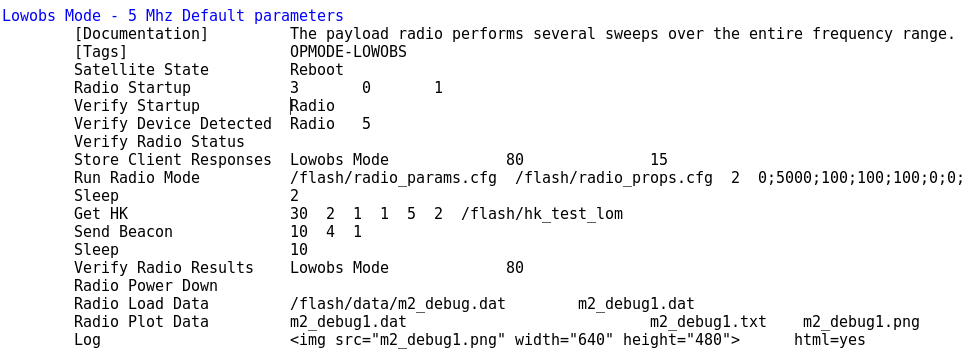
\includegraphics[scale=0.5]{payloadrfwtest}
%\caption{Robot Framework test case structure for radio payload testing.}
%\label{robotradio}
%\end{figure}
\begin{figure}[h!]
\centering
\begin{minted}[fontsize=\small ,tabsize=2,breaklines]{robotframework}
*** Test Cases ***
Lowobs Mode - 5 Mhz Default parameters
	[Documentation]		The payload radio performs several sweeps over the entire frequency range.
	[Tags]				OPMODE-LOWOBS
	Satellite State		Reboot
	Radio Startup		3	0	1
	Verify Startup		Radio
	Verify Device Detected	Radio 	5
	Verify Radio Status
	Store Client Responses	Lowobs Mode		80		15
	Run Radio Mode			/flash/radio_params.cfg  /flash/radio_props.cfg  2  0;5000;100;100;100;0;0;
	Sleep			2
	Get HK			30  2  1  1  5  2  /flash/hk_test_lom
	Send Beacon		10  4  1
	Sleep			10
	Verify Radio Results	Lowobs Mode		80
	Radio Power Down
	Radio Load Data 	/flash/data/m2_debug.dat 	m2_debug1.dat
	Radio Plot Data 	m2_debug1.dat 				m2_debug1.txt	 m2_debug1.png
	Log		<img src="m2_debug1.png" width="640" height="480">	html=yes
\end{minted}
\caption{Robot Framework test case structure for radio payload testing.}
\label{robotradio}
\end{figure}
Most interesting information about the payload operation was found from the CSP client replies outputted to the log files. What was measured was static and as such, nothing too much could have been said about the test cases just by looking the measurement plots. Beyond the fact that the values were not zero or that there was actual variance in the values measured. In Figure \ref{m1_debug1joo} below is one plot produced from measurement made with the radio while the satellite was at the laboratory at Aalto University and no external radio signal sources were generated for testing.\par 
\begin{figure}[h!]
\centering
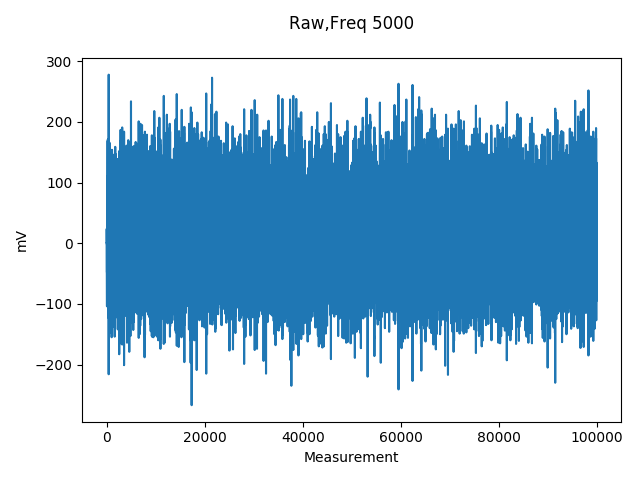
\includegraphics[scale=0.6]{m1_debug1}
\caption{Plot of 100 000 measurements of radio static made by the radio payload at 5 MHz. The vertical axis gives electric field in millivolts.}
\label{m1_debug1joo}
\end{figure}
During integration and testing of the radio payload, several problems occurred. Some of these problems can be attributed to be \textit{emergent problems in integration}. For one, the payload was developed so that a \textit{RaspberryPi 3} computer simulated the OBC. This computer has a Quad Core 1.2 GHz processor from Broadcom \cite{raspi3} and the processor in the NanoMind OBC in Suomi100 is a 32 MHz processor with a single core \cite{nanomindds}. The data from the payload can be read and stored within the 31.25 microseconds with the RaspberryPi 3 in order to have a sample rate of 32 kHz at lowest. But, the reading and storing with NanoMind takes considerably longer, over 60 microseconds approximately. In addition, the data needs to be read two times before obtaining a completely new measurement value. This is because the payload outputs the data from two audio channels, left and right, and data is read from one channel at a time. Therefore, with the NanoMind OBC, a sample rate of approximately 8.3 kHz can be obtained theoretically. Straightforward calculation for this sample rate can be seen in Equation \ref{sampratecalc}. \par
\begin{equation}
\frac{1}{\textrm{data reading and storing time (s)}\times2} = \frac{1}{60 \mu s\times2} \approx 8.3 \textrm{ kHz}
\label{sampratecalc}
\end{equation}
In addition, it was found that the reading and storing even at this rate is not consistent as the FreeRTOS runs other tasks while data is read from the payload. Figure \ref{payloadosc1} shows a screenshot from a \textit{Tektronix TBS 1072B-EDU} oscilloscope reading the \textit{slave select} pin from the payload. When the value of the slave select is low, a single reading of data from the instrument has happened.
\begin{figure}[h!]
\centering
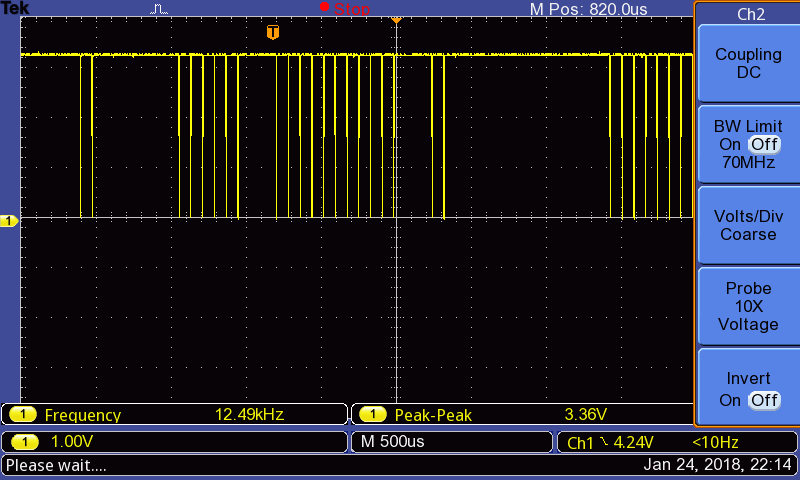
\includegraphics[scale=0.5]{F0001TEK}
\caption{Screenshot from a Tektronix oscilloscope showing inconsistency in data reading rate from the radio payload instrument.}
\label{payloadosc1}
\end{figure}
In an attempt to counter the inconsistent reading, priority of the FreeRTOS task assiocated with the operations of the radio instrument was increased to highest among all of the tasks in NanoMind. This didn't improve the situation though. Thus, the task was made to call for a FreeRTOS \textit{vTaskSuspendAll()} command, which would give all the processing power of the processor for the radio operation task and freeze all the other tasks in the OBC. This caused an unidentified \textit{watchdog} task to reboot the computer, which possibly assumed that the computer was "frozen" and as a safety feature rebooted the computer.\par
Therefore, as a compromise the sample rate was dropped down to 1 kHz. This was done by adding a \textit{vTaskDelay(1)} command to the FreeRTOS task of the radio payload operation after every read and store cycle. This was the shortest time that could be add to the radio operation task, a shorter wait time would have possibly given a higher sample rate. But this would have required modifications to be done to the general definitions of the NanoMind code, which could have caused unforeseen consequences to the operation of the satellite. Figure \ref{payloadosc2} shows that on certain periods data can be obtained more consistently. Yet, during a longer time period, there still exists longer gaps between data reading events than what were anticipated. Nonetheless, this data rate was felt to be good enough for the scientific needs. Though, recording any proper "real-time" human listenable radio signal such as speech or music is not feasible with this setup. With 1 kHz sample rate the signal data doesn't have enough resolution for the signal to sound reasonable by human ears. \par
\begin{figure}[h!]
\centering
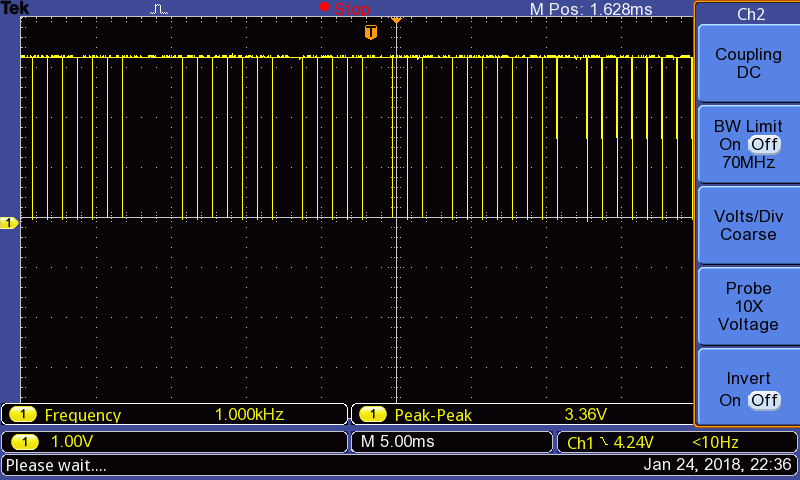
\includegraphics[scale=0.5]{F0003TEK}
\caption{Screenshot from the oscilloscope showing better consistency with lower sample rate in data reading rate from the radio payload instrument.}
\label{payloadosc2}
\end{figure}
In addition to the data rate problem, some problems were discovered with the payload and the Nanomind themselves. For the command to tune the frequency in the Si4740 IC, an automatic antenna capacitance calculation was supposed to happen for a given frequency. Yet, from the Robot Framework log files it was found that the antenna capacitance value was always $1$. Thus, a separate routine had to be written to the NanoMind which calculates the capacitance value. In the consequent tests with this modification, the values seemed to be correct and it could also be seen from the figures plotted from the measurement data.\par 
Another issue which was encountered involved the GPIO pins in the NanoMind. The radio payload would have needed four pins, yet only three out of six worked. Yet, changing the purpose of these three pins in relation to the radio instrument was sufficient. This made it possible for data to be read from the instrument in the first place.\par 
As a conlusion to the radio payload, the subsystem would have required its own processor and its own flash memory in order to have higher sample rate and with more consistent data reading and storing. As is the case with the NanoCam subsystem, which has a 536 MHz processor and 2 Gigabytes of non-volatile memory for image storage. Nonetheless, even with a very low sample rate, valuable information from the Ionosphere can be gathered \cite{esanpapru}.    
\subsubsection{Satellite basic operations}
Testing of the basic functionalities of the satellite software is necessary in order to obtain a reliable satellite \cite{Swart1, smallsatconf31, ecss}. Therefore, tests were performed for satellite platform features such as safe satellite reboots, different housekeeping commands, flight planner commands and flight software updating. All of these can be seen as the basic functionalities which all of the other operations of the satellite depend upon. No requirements were defined by us for these features, therefore this testing is informal in nature. Nonetheless, execution of these tests was felt to be necessary.\par 
Test suites for these features don't follow the combinatorial testing methods used for the two payload subsystems. Instead, test cases are based on different use cases or different situations which the satellite might face. In addition, the keywords used were less subsystem specific and more of the test cases used the generic keywords, such as \textit{Send Command} and \textit{Verify Reply Contained}.\\
\\
\textbf{Reboot tests}
\\
Twelve test cases were written for satellite reboots during different situations. The goal of these tests was to find out if during some operation, e.g. file upload, the NanoMind can become "frozen" so that it doesn't reboot safely anymore. This test suite additionally has test cases only for shutting down different subsystems and to verify their absence in the satellite bus with the \textit{ping} command. From these test cases, it was found that the NanoCom communication system couldn't be shutdown completely. It still replied to the ping commands even though a command was sent to shut it down. This functionality naturally is preferable and though this led to one test case of the reboot test suite to fail, the test can be seen to fail positively. As such, eleven test cases passed and one failed positively from this test suite. Few Robot Framework test cases are presented in Figure \ref{robotreboot}. \par
\begin{figure}[h!]
\centering
\begin{minted}[fontsize=\small ,tabsize=2,breaklines]{robotframework}
*** Test Cases ***
EPS reboot
	[Documentation]		Reboot satellite by rebooting EPS
	[Tags]				OPMODE-POWER
	Satellite State 	Unknown
	Send Command		reboot 2
	Verify Reply Contained 	Welcome to nanomind
    Wait Until Reply Contains   Mount ok

OBC reboot
	[Documentation]		Reboot nanomind OBC
	[Tags]				OPMODE-POWER
	Satellite State 	Unknown
	Send Command		reboot 1
	Verify Reply Contained 	Welcome to nanomind
	
Reboot occuring during file upload
    [Documentation]         Reboot satellite during file transfer
    [Tags]                  OPMODE-COM
    Satellite State         Reboot
    Send Command            cmp route_set 1 1000 8 1 KISS
    Send Command            fp server 1 18
    Create Flight Plan      Reboot   reboot 2  30
    Send Command            ftp server 1
    Send Command            ftp upload_file nanomind2.bin /flash/nanomind_up.bin
    Wait Until Reply Contains  Welcome to nanomind
    Wait Until Reply Contains   Mount ok
    Wait Until Reply Contains   Timeout
\end{minted}
\caption{Robot Framework test case structure for radio payload testing.}
\label{robotreboot}
\end{figure}
The other types of test cases in the reboot test suite tested reboots during satellite operations and the reboots were mostly caused by adding reboot commands to the flight planner so that they would occur during some satellite operation, e.g. during radio payload operation. In all of these, the satellite came back safely. Yet, it has been witnessed several times by us that the NanoMind can get stuck and in those situations to get the OBC working again, it has required manual rebooting of the EPS or sending of a command via another subsystem to reboot the NanoMind. The satellite has recovered safely from these situations after reboot. Fortunately, when using the CSP client over the radio link, rebooting of the system has been possible. Nonetheless, this situation brought up the question whether there can happen something during orbit that causes the satellite to be "frozen" forever.\par
There are several watchdogs in the satellite that in theory can trigger a reboot after a certain time. Unfortunately, a situation couldn't have been deliberately triggered where NanoMind is stuck and thus tests for these watchdog functionalities had to be omitted from the test suite.\\
\\
\textbf{Housekeeping tests}
\\ 
Another eleven test cases were performed to test the housekeeping features provided by the GomSpace platform. Test cases were written for different housekeeping commands of different subsystems as well as for housekeeping data storing and transfer from the satellite. Testing of the beacon functionality was as well included in this test suite, as the beacon outputs recent HK information. Two test cases are presented in Figure \ref{robothk}. \par
\begin{figure}[h!]
\centering
\begin{minted}[fontsize=\small ,tabsize=2,breaklines]{robotframework}
*** Test Cases ***
Download and verify housekeeping
	[Documentation]		Call EPS housekeeping routine
	[Tags]				OPMODE-POWER
	Satellite State 	Reboot
	Send Command 		cmp route_set 1 1000 8 1 KISS
	Send Command 		ftp server 1
	Run Keyword And Ignore Error 	Send Command 	ftp rm /flash/hk_robot.dat
	Send Command 				rparam download 1 19
	Set Satellite Parameter		Nanomind	col_en 	1
	Set Satellite Parameter		Nanomind	store_en 	1
	Send Satellite Parameters
	Send Command 		hk get 0 1 1 0 /flash/hk_robot.dat
	Sleep 				5
	Send Command 		ftp server 1
	Send Command 		ftp download_file /flash/hk_robot.dat hk_robot.dat
	Sleep 				5
	Verify Reply Contained	  	1/1

Get EPS HK directly
	[Documentation]				Call EPS housekeeping routine directly
	[Tags]						OPMODE-POWER
	Satellite State 			Unknown
	Send Command 				cmp route_set 2 1000 8 1 I2C
	Send Command 				eps hk
	Verify Reply Contained 		Voltage
	Send Command 				eps hksub vi
	Verify Reply Contained 		Vbatt
	Verify Reply Contained 		Isun
	Verify Reply Contained 		Isys
\end{minted}
\caption{Robot Framework test case structure for radio payload testing.}
\label{robothk}
\end{figure}  
Plotting of the beacon data was developed during the realization of these tests by another member of the satellite team, M.Sc Petri Koskimaa, and by the thesis author. These plotting functionalities were later used in the "Day in the life of the satellite"-tests as well. All test cases of this test suite passed without errors. This means that, all the commands did what they were supposed to execute, which was obviously the preferred result. In Figure \ref{hkcamplotjoo} we have an example picture of a plot of the system current provided by the beacon at different timestamps. At certain points in time there are ten datapoints due to the beacon feature used in the way that it takes multiple pulls of the system state when it is called. An average for the milliamperes is presented by the dashed red curve. The time is presented in the vertical axis in \textit{Unix} time format. Implying the time in seconds that has elapsed since 1st of January 1970 \cite{linuxproginterface}. The time is in this format because the satellite tracks time in Unix time \cite{nanomindds}.\par 
At the first beacon data collection at approximately 760 seconds, if the presentation of the full Unix time is omitted, the satellite has been restarted by power cycling the EPS and housekeeping data collection has been turned on. Right prior to the next data point at 825 seconds the NanoCam has taken a picture and the same operation was performed right before beacon collection at subsequent points approximately at 875 and 925 seconds. In addition, there was a 20 second wait time between each operation of the camera. From the curve presenting the average of the currents collected via the beacon, it can be seen that operating the camera payload increases the overall current in the satellite system.
\\
\begin{figure}[h!]
\centering
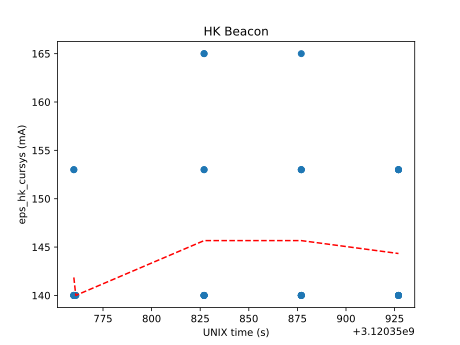
\includegraphics[scale=0.7]{hk_plot_cam_op2_mod}
\caption{System current from the beacon data during imaging mode operation mode. The vertical axis shows system current in milliamperes. Time is shown in seconds since beginning of Unix time. Average for the system current is presented by the dashed red curve and blue dots illustrate singular data points.}
\label{hkcamplotjoo}
\end{figure}
\\
\textbf{Flight planner tests}
\\ 
For testing of the flight planner feature, seven test cases were performed. The feature was tested with some basic flight planner creation commands as well as with more complicated ones. Out of all these tests involving basic functionalities of Suomi100, this one had the most failed test cases. For first, it was assumed that giving the commands in wrong format (string instead of an integer) would cause the CSP client to indicate an error. Such a thing didn't happen but giving the commands in wrong format didn't cause the software to crash either. In addition, if the command string was too long, an error was indicated and no flight planner command was appended to flight plan list. Which happened to be the case with one specific command for the radio payload, but this command to run the radio payload in one of the defined operation modes happens to be the single most essential command for the payload. Therefore, in order to make it work the source code for the flight planner was modified so that it can accept longer strings as commands. Otherwise, the radio payload can be used only when the satellite is in the reach of the groundstation communication radios. This is not preferrable as the area of the Ionosphere that can be measured would be radically limited.\\
\textbf{Software update tests}
\\ 
Three test cases were performed for the software update feature. These tests took the longest time to execute as new software had to be uploaded to the satellite in each test case. These cases tested basic uploading of a new software image, rebooting back to the software that was flashed to NanoMind and tested uploading of an invalid file as an image to the new software. The satellite passed all these tests as expected, giving some confirmation that a new software can actually be safely uploaded to the satellite and the OBC can be commanded to reboot with that software. \par
In the test case where an invalid file was uploaded as an image, the file itself was just a binary file containing measurement values from the payload radio. Booting with this file caused the NanoMind to reset with EXCEPTION 13 error message. In addition, the NanoMind was set to try to boot with this file three times and it reset each time with this error. Eventually as the boot counter reached zero, the satellite managed to recover the proper software it was flashed with. This test provided knowledge that the satellite manages to recover itself if a software happens to be uploaded to the satellite that causes unexpected reboots.\par
\subsubsection{"Day in the life" operational scenarios}
Test suites were formed to test different phases of the scenarios that the satellite will encounter while in orbit. A scenario would be e.g. where the satellite travels in the orbit to the reach of the groundstation, commands are sent to the satellite and data is downloaded. Each step in the scenario, such as downlinking of data, formed its own test case within the test suite. 
Four different operational scenarios were tested. These are described as:
\\
\par 
\textit{1. scenario: The satellite comes from eclipse and is in the reach to form a radio link with the groundstation. Housekeeping data is gathered, the satellite takes an image and a measurement is made with the radio payload. Afterwards, the housekeeping data and the measurement are downloaded from the satellite. Finally, the satellite goes out of the reach of the groudstation.}
\\
\par 
\textit{2. scenario: The satellite comes from eclipse and is in the reach to form a radio link with the groundstation. Housekeeping data is gathered and flight planner is used to set the camera to take a picture while the satellite is in eclipse and out of the reach of the groundstation. After the satellite has orbited the Earth, the satellite comes again from the eclipse and is in the reach of the groundstation. Housekeeping data and the taken image is downloaded from the satellite. The satellite goes again out from the sight of the groundstation.}
\\
\par 
\textit{3. scenario: The satellite comes from eclipse and is in the reach to form a radio link with the groundstation. Housekeeping data is gathered and flight planner is used to set the camera to take pictures continuosly. Flight planner is used to gather housekeeping data continuosly as well. A sudden reboot happens and presence of all subsystems is verfified after restart. The camera is given a command to take a picture to verify the basic operation of the subsystem. In addition, verification for the charging of the batteries via the solar panels is verified. Finally, the housekeeping data is downloaded from the satellite.}
\\
\par 
\textit{4. scenario: The satellite comes from eclipse and is in the reach to form a radio link with the groundstation. Housekeeping data is gathered and a file is uploaded to the satellite. Finally the satellite goes out of sight of the groundstation.}\\
\\
One test suite for each scenario was written. Different phases of a scenario were made in to different test cases in the suite. Majority of the keywords used in the test suites were the \textit{Persistent Command} and \textit{Verify Reply Contained} keywords. Persistent commanding was required for majority of the commands because the radio link was not entirely stable. The test suites were executed several times and occasionally some keywords caused the test cases to fail due to the connection being temporarily lost. A complete test suite for the first scenario can be seen in Appendix \ref{LiiteB}.\par
Control of the solar simulator was not automated due it being simply a lamp that one attaches to the electric plug to turn it on. Thus in practice the person responsible for the testing had to manually plug and unplug the simulator from the mains current. Therefore, another keywords were written for these tests which with a sound effect indicate that the lamp has to be turned on or to be turned off according to the time periods explained in section 3.3.4. These are the \textit{Wait And Notify}, \textit{Notify After}, \textit{Wait Until Time event} keywords.\par
One important aspect with these tests was verification that the solar panels charge the batteries. All the test suites had at least one test case for battery charging verification. In all such cases, the solar panels were detected and they did infact charge the batteries. As presented in section 2.1, one of the potential causes for failures with previous CubeSats has been that the solar panels were not properly connected to the power bus \cite{Swart1}. Thus, testing of this was felt to be crucial.\par 
Figure \ref{epsvbatt} shows how the charge in the batteries changed over the execution of the first scenario. There are ten data points at each point in time where the beacon feature was called. The dashed red curve shows average of the recorded millivolts. The time is presented in the vertical axis in \textit{Unix} time format. If presentation of the full Unix time is omitted, at approximately 160 seconds the first housekeeping data through the beacon has been gathered. Recently prior to this, the OBC has been restarted. Before the consequent points at approximately 220 and 225 seconds, nothing more than housekeeping collection features have been turned on.\par
At approximately 255 seconds the battery voltage shows an increase, which indicates that the solar panels have begun to recharge the batteries. In addition, prior to this data collection the camera was operated and the taken image was stored to the NanoCam. flash drive. An increase is again shown at the next housekeeping collection at approximately 380 seconds. Before this point in time, the ADCS has been turned off and the radio payload has ran second mode of the radio operation modes. The final collection point was taken after radio measurement data had been downloaded. It can been seen from the dashed red curve that the battery voltage shows a steady increase when the satellite was under illumination, even though the satellite operated both of its payloads during this time.  
\par
\begin{figure}[h!]
\centering
%\includesvg{hk_plot1_mod}
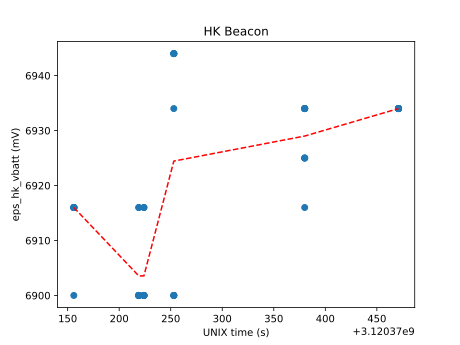
\includegraphics[scale=0.7]{hk_plot1_mod}
\caption{EPS battery charge from the beacon data during the first satellite operational scenario. The vertical axis shows system voltage in millivolts. The red dashed curve presents average of the battery voltage and blue dots illustrate singular data points. Time is shown in Unix time in the horizontal axis. }
\label{epsvbatt}
\end{figure}  
Concurrently, all the test cases for scenario 1 were executed succesfully. The housekeeping data and radio measurement were downloaded from the satellite succesfully via the radio link. Similarily, all test cases for scenario 3 succeeded. A reboot was caused in the satellite and all the subsystems responded to \textit{ping} commands after the reboot. The satellite was able to again take an image and it was verified that the solar panels were again charging the satellite. Test cases for scenario 4 were passed as well and a file was uploaded succesfully to the satellite.\par 
Some problems emerged with testing of scenario 2. Namely, the download speed was too slow to enable downloading of an image from the satellite during the time defined for the scenario. As presented in section 3.3.4, the time that the satellite is in the sight of the groundstation is approximately 10 minutes. The image taken by the camera was roughly 300 kilobytes in size and during the time it was downloaded, roughly 53 kilobytes was received.\par 
One reason for the slow download speed was the setting for CSP client \textit{rdpopt} command, which controls the wait times between each packets received and other commmunication related features. With a short wait time the time between received packets is shorter, but the connection during downloading can be lost more frequently. With a longer wait time, the speed is lower but the connection is more stable. The theoretical maximum speed for downloading data with the bandwidth allocated for Suomi100 mission is $0.9 kb/s$. From the test suite logs produced by the Robot Framework, it could be seen that at best data could be received at the speed of $0.3 kb/s$. Therefore, fine tuning of the \textit{rdpopt} command's parameters would be needed in order to make the download faster in practice.\par
As a conclusion, it was verified that the solar panels did charge the batteries and the communication with the satellite over the radio link worked. All the commands sent to the satellite worked as they were supposed to according to the GomSpace manuals. Only the download speed was slow with the parameters given to the \textit{rpopt} command in the test. Thus, a full picture couldn't be downloaded from the satellite. Besides this, all the test cases passed.\par      
\subsection{Release version of CubeSatAutomation test library}
As was already stated in \textit{Research purpose and goals} in Section 1, the goal was to create a reusable test automation function library. Other satellite teams working with testing of their systems could utilize this funtion library along with Robot Framework to automize and bring a systematic nature into their testing. 
Basis for this library was the libraries used in testing of Suomi100 and several features were preserved while others were omitted from the final function library. Notably, all the Suomi100 specific keywords and routines were removed. In addition, some changes to the preserved keywords were made.\par 
One essential change was the completion of the network socket based communication with the system under test. With the core library used in testing of Suomi100, only the stdin was used when replies were read from the CSP client. In the final \textit{CubeSatAutomation} library, replies from a program can be read through the socket connection as well. In addition, several of the keywords try to choose the communication between network socket and stdin/stdout console communication. If a socket object is found to be defined in the class variables of the function library, then socket connection is used for sending commands as well as receiving responses from the SUT. If not, stdin/stdout is used for the communication, with no visible difference in the keywords when they are called in the test cases. The socket communication was tested to work with RaspberryPi 3 through an \textit{Ethernet} cable. For this purpose a program using the source code listed in Appendix \ref{LiiteD} was written to the RaspberryPi as a crude \textit{endpoint} software.  \par
Having two methods of communication with the system under test gives certain benefits. For example, a groundstation software or a flight software in a simulated desktop environment can be tested locally by using the console communication. When using the network socket for communication with the SUT, testing can be performed on the target hardware (e.g. a subsystem or an integrated satellite) as well if the hardware has networking capabilities. A separate computer which has networking capabilities could be used for directly controlling the target hardware if the SUT doesn't provide methods for network connection. \par 
To support testing on a remote system, new keywords for remote program startup and termination were developed. For these operations, the keywords use the \textit{Secure Shell} (SSH) communication provided by the Python \textit{Paramiko} library. This communication method is only used for the aforementioned actions, but a future update to the library could additionally include SSH based command sending and response receiving. \par 
Naming of certain keywords was changed as well. The keywords related to program startup and shutdown now have a more generic \textit{Program} as the first word. \textit{Client} was used as the first word in the original version due to the groundstation software being named CSP client. In addition, configuration files could be passed to certain keywords in the Suomi100 test automation libraries and that feature is preserved in the release version as well. The keywords related to program and socket setup accept configuration files as keyword arguments. When such a file is given, the content of the file overrule any other arguments passed to the keyword. The source code for the final CubeSat test automation library is listed in Appendix \ref{LiiteA} along with example of a configuration file. In future the library could be written to be more modular with the class methods separated into different Python modules. Listing of such implementation was felt to complicate the source code presentation in the Appendix of this thesis.\par
However, the source code was added to a \textit{Git} at \url{https://github.com/Juha-MattiLukkari/cubesatautomation}. New versions of the test automation library with improvements written to it can be obtained from this website. In addition, Robot Framework examples of how the library can be utilized in testing exist in the Git. \par
In Robot Framework format, the keywords available in the final function library are the following:\\
\textit{\textbf{Program Start  <program> <parameters> <config file> <wait>}}\\
Starts the program that is to be automated. Parameters to the program can be defined and both of the arguments can be read from a configuration file. Wait for \textit{<wait>} seconds to let the program start properly.\\
\textit{\textbf{Program Close}}\\
Closes the program and a possible socket assiocated with it.\\
\textit{\textbf{Connect Socket  <server> <port> <config file> <wait>}}\\
Opens a socket connection to a defined server and port address. These values can be read from a configuration file as well. Wait for \textit{<wait>} seconds to let the connection be established fully.\\
\textit{\textbf{Close Socket}}\\
Closes the opened socket connection.\\
\textit{\textbf{Remote Program Start  <program> <server> <port> <username> <password> <config file> <wait>}}\\
Starts a program on a remote server using SSH. All the arguments for this keyword can be read from a config file. Wait for \textit{<wait>} seconds to let the program start properly.\\
\textit{\textbf{Remote Program Close}}\\
Closes the SSH connection and terminate the opened program at the remote system.\\
\textit{\textbf{Send Command  <message> <option> <timeout> <read timeout>}}\\
Sends a message and read replies through socket connection. The reply can be stored temporarily or discarded. Read replies for \textit{<timeout>} seconds, with \textit{<read timeout>} seconds between each attempt to read data.\\
\textit{\textbf{Write Command  <message> <option> <timeout> <read timeout>}}\\
Writes a command to the standard input and reads a reply from the standard output. The reply can be stored temporarily or discarded. Read replies for \textit{<timeout>} seconds, with \textit{<read timeout>} seconds between each attempt to read data.\\
\textit{\textbf{Type Command  <message> <option> <timeout> <read timeout>}}\\
Types a command by automating keypresses on the keyboard and reads a reply from the standard output. The reply can stored temporarily or discarded. Read replies for \textit{<timeout>} seconds, with \textit{<read timeout>} seconds between each attempt to read data. \\
\textit{\textbf{Persistent Command  <message> <exception replies> <end reply> <timeout> <read timeout>}}\\
Writes a command persistently to the SUT through the communication method defined earlier until a defined reply is read, a specific error reply is read or a timeout value is reached.  Try to read replies for \textit{<read timeout>} seconds between each attempt.\\
\textit{\textbf{Verify Reply Contains  <message> <timeout> <read timeout>}}\\
Reads several lines through the established communication route and tries to find for a defined message from the lines. Read replies for \textit{<timeout>} seconds, with \textit{<read timeout>} seconds between each attempt to read data.\\
\textit{\textbf{Verify Reply Contains Not  <message> <timeout> <read timeout>}}\\
Reads several lines through the established communication route and tries not to find for a defined message from the lines. Read replies for \textit{<timeout>} seconds, with \textit{<read timeout>} seconds between each attempt to read data.\\
\textit{\textbf{Verify Reply Contained  <message>}}\\
Tries to find a defined message from the replies that were stored by an earlier command. \\
\textit{\textbf{Verify Reply Contained Not  <message>}}\\
Tries not to find a defined message from the replies that were stored by an earlier command. \\
\textit{\textbf{Wait Until Reply Contains  <message> <timeout> <read timeout>}}\\
Reads replies through the established communication route until a defined message is found or a timeout is reached. Read replies for \textit{<timeout>} seconds, with \textit{<read timeout>} seconds between each attempt to read data.\\\\
\textit{\textbf{Clear Messages  <option> <read timeout>}}\\
Reads messages through socket for \textit{<read timeout>} seconds and discards them. Replies that were stored earlier can be chosen to be removed.\\
\textit{\textbf{Clear Replies  <option> <read timeout>}}\\
Flushes the standard output and reads replies for \textit{<read timeout>} seconds and discards them. Replies that were stored earlier can be chosen to be removed.\\
\textit{\textbf{Clear Stored Messages}}\\
Empties all the stored replies.\\
\textit{\textbf{Save Program Replies  <filename> <timeout> <read timeout>}}\\
Read replies in the background from the program and saves them to a file. Replies are read for \textit{<timeout>} seconds, with \textit{<read timeout>} seconds between each attempt to read data.\\
\textit{\textbf{Verify Saved Reply  <message> <filename> <timeout>}}\\
For \textit{<timeout>} seconds, tries to find for a reply from the file where replies are being saved.\\
%The architecture of the final CubeSatAutomation function library was rewritten as well and the library was written to have larger degree of modularity. This would enable future teams to write new keywords in a fast pace by using only the necessary methods found in the function library. The function library itself was divided into separate modules, with \textit{internal.py} having certain communication related routines, \textit{verifications.py} containing the keywords for program response verifications, \textit{program.py} consisting of keywords for starting and closing of the SUT and \textit{CubeSatAutomation.py} having the keywords for sending commands to the system. Only the \textit{CubeSatAutomation} is required to be included when writing tests with Robot Framework, this library provides access to all methods present in the libraries.\par 
%pip install -r requirements.txt  
%pip install -e . (setup.py tarvitaan) 
\subsection{Improving CubeSat reliability: "Day in the life of a CubeSat" test}
Currently the CubeSat standard demands the following tests to be performed for a satellite: \textit{Random Vibration}, \textit{Thermal Vacuum Bakeout}, \textit{Shock Testing} and \textit{Visual Inspection} \cite{cds}. These are demanded only for the reason of ensuring safe integration of the P-POD deployer and the CubeSat in to the launch vehicle. The specifications for these tests in fact usually are defined by the launch provider \cite{cds}.\par 
As can be seen, no testing is required for electrical or functional/operational testing of the satellite at the system integration level. In the research data represented in section 2.1 it was found that failure rates from 40 \% to 20 \% were prevalent in CubeSat missions \cite{Swart1, Swart2016, Swart2015}. In addition, it was suggested that these high failure rates were attributed to poor or nonexistent functional system integration testing. More so, understanding of integration and testing can be something lacking from the University led CubeSat teams. In comparison, the CubeSat missions that were led by organisations and companies with vast experience in satellite integration and testing had considerably lower failure rates.
Therefore, we are suggesting at least for some form of guidelines for functional system integration testing to be added to the CubeSat project concept. Detailed study for creation of such guidelines is deemed to be necessary. \par
In section 2.1.5, the represented research on failures with larger spacrafts also pointed to the lack of proper integration and testing as a source for mission failures. In addition, when the established testing practices used in NASA were "streamlined", consequent missions showed significant increase in failures. When comparing the data from failed CubeSat and traditional space missions, it could further be claimed that at least some guidelines for system integration testing are needed to be included to the CubeSat project. \par
\subsubsection{Test design}
The "Day in the life" operational scenario tests are required for NASA and ESA missions \cite{tor}. Besides the mechanical tests mentioned, a test following that principle could be devised as a recommended guideline for functional CubeSat testing. This test could be known as \textbf{\textit{"Day in the life of a CubeSat"}}, following the methods described in sections 4.1.4 and 3.3.4. Test such as this would test the functionality and proper integration of the satellite. The communication with the groundstation could likewise be verified. In theory, this test could decrease the amount of DOA cases for CubeSat missions. As noted in \cite{Langer, Swart1} one of the alleged reasons for early CubeSat failures has been improper integration of the solar panels to the satellite and thus not having enough power to form the radio link with the groundstation. A test such as the one discussed here could on ground verify these two aspects of the mission.\par
In fact, a study done in NASA during 2017 came to similar conclusions about a "Day in the life" testing for CubeSats \cite{improvingcubesatsuccess}. A recommendation was set forth for a test such as this by operating the satellite via ground station and performing nominal operations of the satellite. In addition, using a solar illuminator to verify battery charge/discharge was recommended to be included in this test. As noted, these aspects were tested for Suomi100 in this thesis and suggested as a "Day in the life of a CubeSat" test in this thesis. In addition to the study conducted by NASA.\par  
One technical solution for a "Day in the life of a CubeSat" test is presented in this thesis. This includes the integrated satellite, a solar simulator and the groundstation. Certain basic scenarios for satellite operations were devised and tested. The mechanical stress tests for CubeSats are performed with automated machinery, likewise a method to automate "Day in the life of a CubeSat" is presented in this thesis. This test automation includes Robot Framework and the function libraries developed during the course of the thesis. The final version of the function library was made to be a generic testing library, which is able to automate the use of many programs running in terminal environment. Groundstation control software can also be automated with this, given that they are terminal based. In addition, as CubeSats often fall short in resources and time for testing, the solution to automate the testing could help in this aspect as well. A setup for a "Day in the life of a CubeSat" test is presented in Figure \ref{dayinlifediagram}.\par
\begin{figure}[h!]
\centering
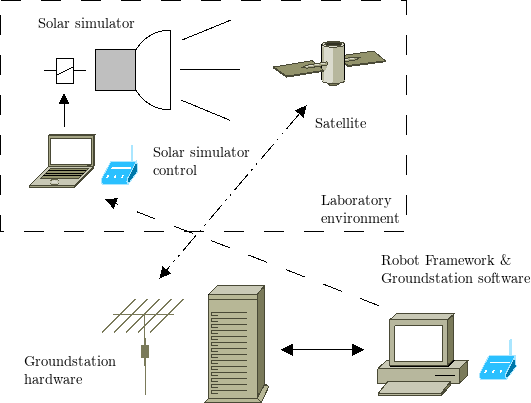
\includegraphics[scale=0.6]{dayinlifesetupdiagram}
\caption{Presentative diagram for a "Day in the life of a CubeSat" test with automated control of groundstation and solar simulator.}
\label{dayinlifediagram}
\end{figure}   
%Documentation for a "Day in the life of a CubeSat" is another aspect that should be considered. Perhaps, the rigorous methods used in NASA [source] could be avoided and a more subtle method could be devised. Starting from design for operational scenarios to features to be tested and finally to documentation of passed and failed test cases.\par
  
% Test suites like the ones were written could be run continuosly over several days even. Thus we could truly make tests for the life of the satellite and automate the whole testing. "Real" satellites could also benefit from this.
\subsubsection{Improved requirements and operational specifications}
Testing to validate the requirements of the Suomi100 mission was informal to some degree, as the requirements were not specified in more detail. Especially testing of the functionalities of the satellite platform was done in an informal manner. No requirements on that level were defined. In addition, in the interest of "Day in the life" testing, no formal documentation about satellite on-orbit operational scenarios were devised.\par 
Therefore, the need for a more detailed requirements and operational documentation was found out as a results of the testing of Suomi100. Yet, the rigour used by the traditional space missions could be avoided. In the vein of the ideology behind CubeSats, an easier and more writable approach towards documentation should also be considered.\par 
Definition of different operation modes and assembling different operational scenarios from them could be beneficial for the "Day in the life" testing. Each operation mode could be further described with more detail: \textit{What should the mode do? What it shouldn't do? Which commands are to be used? What happens on failure? Area of operation?}. Perhaps presenting each operation mode with a \textit{State diagram} or with some other modeling method. In fact, according to \cite{embeddedsofteng}, modeling of a system is preferred if not required for mission- and safety-critical applications.\par 
In conclusion, a design for "Day in the life of a CubeSat" test could consist of the following steps:
\begin{enumerate}
\item Design different on-orbit operational scenarios based on the mission definition.
\item Break different scenarios into different operation modes of the satellite. Modes for example such as \textit{downlink data}, \textit{use payload instrument}, \textit{stay idle} and so forth. Create state diagrams for the operation modes and derive functional requirements from the diagrams.
\item Run a scenario over a radio link and use a solar illuminator to simulate the Sun.
\item Verify battery charging and proper communication with the satellite over the radio link.
\item Based on the operation mode functional requirements, verify proper functionality of different operation modes in a scenario.
\item Perform steps 3-5 for all operational scenarios. 
\end{enumerate}
On the next page an example state diagram of \textit{Imaging mode} operation mode is presented in Figure \ref{imagingstate}. The operation mode is defined in Section 2.4.2. The different states are presented as circles and the status of each subsystem in the satellite is indicated within the circle. Transitions between states are indicated by arrow lines. \textit{Idle} state is the initial state of the system. When a critical failure is caused in the satellite by e.g. software error, the satellite goes into \textit{System shutdown} state and the satellite power cycles the EPS and restarts the OBC and other subsystems. The satellite finally returns to the Idle state after the reset.

\begin{figure}[h!]
\centering
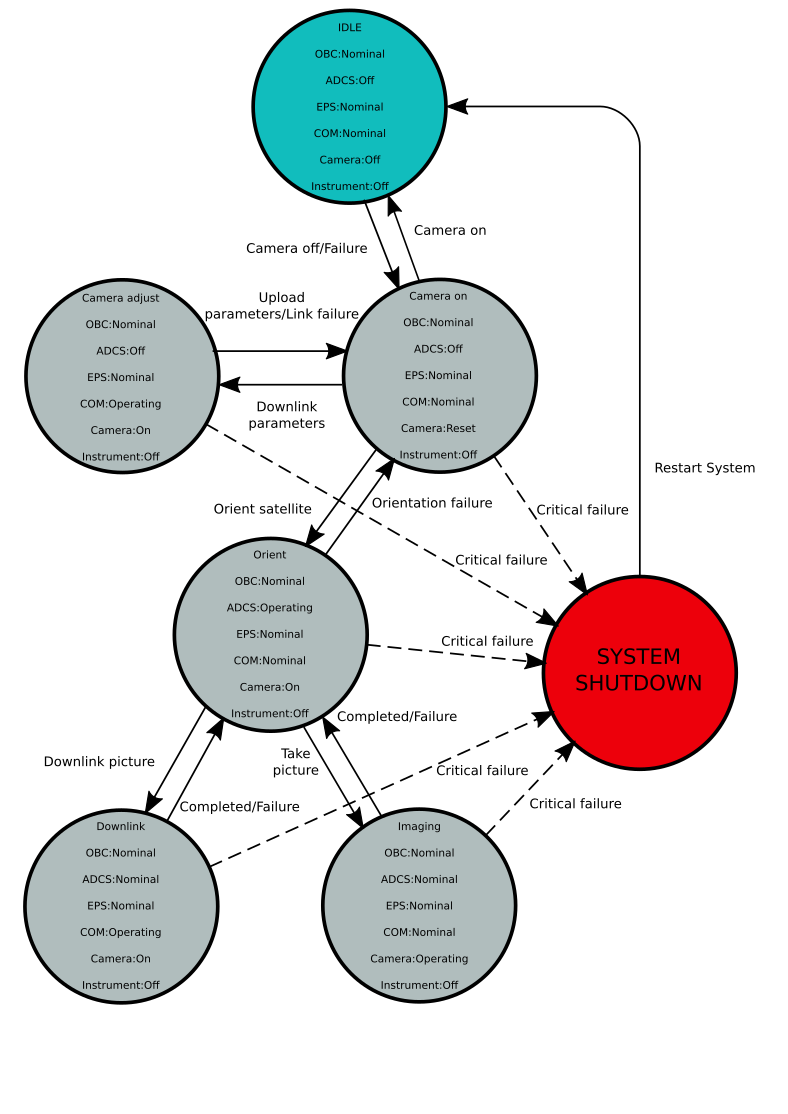
\includegraphics[scale=0.6]{imagingstate}
\caption{The \textit{Imaging mode} operation mode as a State diagram. Circles represent states of the satellite and arrow lines indicate transitions between each state. }
\label{imagingstate}
\end{figure}   
 


%% Huomaa seuraavassa kappaleessa lainausmerkkien ulkopuolella piste, 
%% koska piste ei lopeta lainattua tekstinp\"atk\"a\"a.
%% Jos lainattu tekstinp\"atk\"a loppuu v\"alimerkkiin, tulee v\"alimerkki
%% lainausmerkkien sis\"alle: 
%% "Et tu, Brute?" sanoi Caesar kuollessaan.


\clearpage

\section{Conclusions} 
%\section{Yhteenveto}
In this thesis automated functional system integration tests for Suomi100 CubeSat were performed with Robot Framework. The need for testing at this level was identified from surveys conducted for all CubeSat missions flown previously, which showed a high failure rate for University led missions in contrast to low failure rates for missions performed by organisations and companies with established practices in integration and testing. Thus, testing methods used by e.g. NASA at satellite integration level along with industry proven testing practices were applied in design of testing performed for Suomi100. The testing was automated with Robot Framework, which is an industry proven open source test automation framework. The framework can be freely obtained through \url{http://robotframework.org/#introduction}. It was felt that doing the testing with the help of an automated computer software would give the testing more rigour and reproducability. Reusable function libraries that were used in automation of the testing were written with Python programming language. Reusable version of the test automation software can be obtained from \url{https://github.com/Juha-MattiLukkari/cubesatautomation}.\par
First tests conducted for the satellite were functional tests for integrated Suomi100 payloads, which are an optical white light camera and an AM radio instrument for ionospheric measurements. Second test set included testing of the core satellite functions  such as housekeeping data collection, safe reboot handling, software updates and so forth. Final set consisted of tests for operational mission scenarios or "Day in the life of the satellite"-tests.\par 
The thesis described the work which was done to simulate the functional environment for testing of the payloads and the operational scenario tests. For testing of the camera payload, the satellite was taken to a balcony at Aalto University on a sunny day. During the testing of the integrated radio payload,  a HackRF software defined radio was used to simulate the noise signals found in the Ionosphere. A larger setup was used for the "Day in the life of the satellite"-tests. With this test, not just the proper functionality of the satellite software was tested but that the radio link to the satellite works and that the solar panels can charge the satellite. As such, the automated tests were performed via the radio link and a large Xenon lamp was used to simulate the Sun.\par 
With the performed tests, we proved proper functionality of the camera payload as well as proper functionality for almost all of the tests conducted for the core satellite functions.   The operational scenario tests showed that we can communicate with and send commands to the satellite via radio link and that the solar panels can charge the batteries in Suomi100. Only downside seemed to be the low downlink speed, yet this was to be expected.\par 
The tests for the radio payload on the other hand presented several defects and most importantly emergent problems in the integration with the rest of the satellite platform. The defects were resolved with consequent software updates, but certain problems with integration couldn't be overcome. The biggest one being the slow speed of reading and storing of data from the payload by the OBC. This demanded decreasement of the sample rate from the possible 32-48 kHz to just 1 kHz for reliable data measurement.\par  
Performing these tests proved to us that Robot Framework can work as a testing framework for CubeSats and that we could carry out automated testing of Suomi100 CubeSat. The software libraries doing the actual automation were developed into a generic testing library, which potentially could be used for testing and automation of any Linux terminal software, such as a satellite ground station control software.\par 
A solution for improving the success rate of CubeSat missions through testing was presented in this thesis as "Day in the life of a CubeSat" test. Furthermore, features that are to be tested are proposed to be defined through state diagrams. The diagrams would represent different operation modes of the satellite and functional requirements of the system could be derived from the state diagrams. In order to decrease failure rates of CubeSat missions, these two tasks are proposed to be added as part of the CubeSat concept as guidelines for system integration testing. \par 
The "Day in the life of a CubeSat" tests the functionalities which have from statistics been considered as causing the infant mortality of CubeSats. In the test mentioned, the ground station is used to control the satellite over the radio link and the satellite is situated in a laboratory with a solar illuminator. By executing nominal satellite operations with this setup, the proper on-orbit functionality of the satellite can be verified. As noted, technical solution for automating this test by automating the control of the groundstation software is presented in this thesis.




\clearpage
%% L\"ahdeluettelo
%%
%% \phantomsection varmistaa, ett\"a hyperref-paketti latoo hypertekstilinkit
%% oikein.
%%
%% The \phantomsection command is nessesary for hyperref to jump to the 
%% correct page, in other words it puts a hyper marker on the page.

\phantomsection
\addcontentsline{toc}{section}{\refname}
%\addcontentsline{toc}{section}{References}
\begin{thebibliography}{99}

%% Alla pilkun j\"alkeen on pakotettu oikea v\"ali \<v\"alily\"onti>-merkeill\"a.
\bibitem{aftersputnik} Collins, Martin,
  \textit{After Sputnik: 50 Years of the Space Age}, Smithsonian Books, HarperCollins, New York, USA, 2007.
\bibitem{rocketeers} Belfore, Michael,
  \textit{Rocketeers: How a Visionary Band of Business Leaders, Engineers, and Pilots Is Boldly Privatizing Space}, \nth{1} edition, Smithsonian Books, HarperCollins, New York, USA, 2007.
\bibitem{accesstospace} Herrell, Linda M.,
  \textit{Access to Space for Technology Validation Missions: A Practical Guide}, Jet Propulsion Laboratory, 2007 IEEE Aerospace Conference, Montana, USA, 3-10 March 2007. 
\bibitem{pluto} 
  \textit{http://pluto.jhuapl.edu/}, accessed 8th of March 2018. 
\bibitem{satcommunications} Pratt, Timothy, Charles W. Bostian \& Jeremy E. Allnutt,
  \textit{Satellite Communications}, \nth{2} edition, John Wiley \& Sons, New Jersey, USA, 2003.
\bibitem{bouwmeester} Bouwmeester J. et al.,
  \textit{Survey of worldwide pico- and nanosatellite missions, distributions
and subsystem technology}, Delft University of Technology, Acta Astronautica, Vol 67:7-8, 2010.
\bibitem{cubesatevolution} Poghosyan, Armen et al.,
  \textit{CubeSat evolution: Analyzing CubeSat capabilities for conducting science missions}, Skolkovo Institute of Science and Technology, Progress in Aerospace Sciences, Vol 88, 2017.
\bibitem{launchmarket} DePasquale J. et al.,
  \textit{Analysis of the Earth-to-Orbit Launch Market for Nano and Microsatellites}, American Institute of Aeronautics and Astronautics, AIAA SPACE 2010 Conference \& Exposition, California, USA, August 30 - September 2 2010.
\bibitem{cds} The CubeSat Program,
  \textit{CubeSat Design Specification Rev. 13}, California Polytechnic State University, 2014.
\bibitem{filaw} 
  \textit{https://tem.fi/en/spacelaw}, accessed 23rd of February 2018.
\bibitem{iceye}
  \textit{http://markets.businessinsider.com/news/stocks/iceye-successfully-launches-world-s-first-sar-microsatellite-and-establishes-finland-s-first-commercial-satellite-operations-1012996541}, accessed 23rd of February 2018.
\bibitem{Swart2017kalvo} Swartwout, Michael,
  \textit{CubeSats and Mission Success: 2017 Update (with a closer look at the effect of process management on outcome)}, NASA Electronic Parts and Packaging (NEPP) Program
2017 Electronics Technology Workshop, Maryland, USA, 26-29 June 2017.
\bibitem{SpaceWorks2017} Doncaster, Bill \& Williams Caleb \& Shulman Jordan,
  \textit{2017 Nano/Microsatellite Market Forecast}, SpaceWorks Enterprises, Inc. (SEI), Atlanta, USA, 2017.
\bibitem{Swart2016} Swartwout, Michael,
  \textit{Secondary Spacecraft in 2016: Why Some Succeed (And Too Many Do Not)}, Saint Louis University , 2016 IEEE Aerospace Conference, Montana, USA,  5-12 March 2016. 
\bibitem{Langer} Langer, Martin \& Bouwmeester Jasper,
  \textit{Reliability of CubeSats - Statistical Data, Developer's Beliefs and the Way Forward}, \nth{30} Annual AIAA/USU Conference on Small Satellites, 2016.
\bibitem{Swart1} Swartwout, Michael,
  \textit{The First One Hundred CubeSats: A Statistical Look}, Journal of small satellites, 2013.
\bibitem{Swart2015} Swartwout, Michael,
  \textit{Secondary Spacecraft in 2015: Analyzing Success and Failure}, Saint Louis University, 2015 IEEE Aerospace Conference, Montana, USA, 7-14 March 2015. 
\bibitem{s100blogi}
  \textit{http://www.suomi100satelliitti.fi/mika}, accessed 6th of March 2018.
\bibitem{robotmain}
  \textit{http://robotframework.org/}, accessed 28th of January 2018.
\bibitem{nasacubesat1}
  \textit{https://www.nasa.gov/mission\_pages/station/research/benefits/cubesat}, accessed 23rd of February 2018.
\bibitem{openorbiter} Straub, Jeremy et al.,
  \textit{OpenOrbiter: A Low-Cost, Educational Prototype CubeSat Mission Architecture}, Machines 1:1-32, 2013.
\bibitem{reliabilitycubesatelbus} Bouwmeester Jasper et al,
  \textit{Survey on the implementation and reliability of CubeSat electrical bus interfaces}, CEAS Space J, Vol 9:163-173, 2017.
\bibitem{spacesystemsengineering} Fortescue, Peter et al.,
  \textit{Spacecraft Systems Engineering}, \nth{4} edition, John Wiley \& Sons, USA, 2011.
\bibitem{radiohandbook} Silver, H. Ward,
   \textit{The ARRL Handbook for Radio Communications 2016}, \nth{93} edition, The American Radio Relay League, USA, 2015.
\bibitem{csdatabase}
  \textit{https://sites.google.com/a/slu.edu/swartwout/home/cubesat-database}, accessed 19th of March 2018. 
\bibitem{smallsatconf31}
  \textit{http://spacenews.com/cubesat-reliability-a-growing-issue-as-industry-matures/}, accessed 12th of December, 2017. 
\bibitem{ssvi}
  \textit{https://www.nasa.gov/smallsat-institute}, accessed 12th of December, 2017.
\bibitem{failureshistory}
  \textit{http://claudelafleur.qc.ca/Scfam-failures.html}, accessed 3rd of April 2018. 
\bibitem{marsfailures} 
  \textit{https://www.space.com/13558-historic-mars-missions.html}, accessed 23rd of February 2018.
\bibitem{schiaparelli} Tolker-Nielsen, Toni,
  \textit{EXOMARS 2016 - Schiaparelli Anomaly Inquiry}, European Space Agency, 2017.
\bibitem{onorbitfailures} Tafazoli, Mak,
  \textit{A study of on-orbit spacecraft failures}, Acta Astronautica, 64:195-205, 2009.
\bibitem{satsubsystems} Castet, Jean-Francois et al.,
  \textit{Satellite and satellite subsystems reliability: Statistical data analysis
and modeling}, Georgia Institute of Technology, Reliability Engineering and System Safety, Vol 94, 2009.
\bibitem{satverplanning} Tosney, William F. et al.,
  \textit{Satellite verification planning: Best practices and pitfalls related to testing}, Proceedings of the \nth{5} International Symposium on Environmental Testing for Space Programmes, Netherlands, 2004.
\bibitem{whenstandignored} Jackelen George. et al,
  \textit{When Standards and Best Practices are Ignored}, Fourth IEEE International Symposium and Forum on Software Engineering Standards, 1999.
\bibitem{embeddedjokusatellite} Williams, Brian C. et al.,
  \textit{Model-Based Programming of Intelligent
Embedded Systems and Robotic Space Explorers}, Proceedings of the IEEE, Vol 91:1, IEEE, 2003.
\bibitem{sularikurssi} Laplante, Phillip A. \& Ovaska Seppo J.,
  \textit{Real-Time Systems Design and Analysis}, \nth{4} edition, IEEE Press, USA 2012.
\bibitem{embeddedsofteng} Oshana, Robert et al.,
  \textit{Software Engineering for Embedded Systems: Methods, Practical Techniques and Applications}, Newnes, Elsevier, Massachusetts USA, 2013.
\bibitem{testingcomplex} Pries, Kim H. \& Quigley Jon M.,
  \textit{Testing Complex and Embedded Systems}, Taylor and Francis group, CRC Press, USA 2011.
\bibitem{artofsofttesting} Myers, Glenford J.,
  \textit{The Art of Software Testing}, \nth{3} edition, John Wiley \& Sons, New Jersey, USA, 2012.
\bibitem{ieeesofttesting1} ISO/IEC/IEEE 29119-1:2013(E),
  \textit{Software and systems engineering — Software testing — Part 1: Concepts and definitions}, IEEE 2013.
\bibitem{systinttesting1} Kandl, Susanne et al.,
  \textit{A Formal Approach to System Integration Testing}, European Dependable Computing Conference, United Kingdom, 2014.   
\bibitem{softacceptancespace} Wortman, Kristin,
  \textit{Management of Independent Software Acceptance Test in the Space Domain: A Practitioner's View}, 2012 IEEE Aerospace Conference, Montana, USA, 3-10 March 2012.
\bibitem{compinspace} Tomayko, James E.,
  \textit{Computers in Spaceflight: The NASA experience}, National Aeronautics and Space Administration, Wichita State University, USA 1988.
%https://ia800304.us.archive.org/19/items/nasa_techdoc_19880069935/19880069935.pdf
\bibitem{cassinitestbed} Badaruddin, Kareem S.,
  \textit{System Testbed Use on a Mature Deep Space Mission: Cassini}, 2008 IEEE Aerospace Conference, Montana, USA, 1-8 March 2008.
\bibitem{tor} White, Julia D.,
  \textit{Test Like You Fly: Assessment and Implementation Process}, Aerospace Report NO.
TOR-2010(8591)-6, Space and Missile Systems Center Air Force Space Command, El Segundo California, 2010.
\bibitem{ecss} European Cooperation For Space Standardization (ECSS) Secretariat,
  \textit{Space Engineering Verification}, ESA Requirements and Standards Division, ESTEC, Netherlands, 2009.
\bibitem{reliabilitylessonsfromnasa} Williams, W. C.,
  \textit{Lessons from NASA: Design reviews, failure analysis, and redundancy are favored over predictions and life testing for spacecraft success}, IEEE Spectrum, Vol. 18:10, 1981.
% USE THE JACKLIN SOMEWHERE, prolly good
%\bibitem{Jacklin} Jacklin, Stephen A.,
%  \textit{Survey of Verification and Validation Techniques for Small Satellite Software Development}, Space Tech Expo Conference USA, CA, 2015.
\bibitem{testautomationconf2013}, Tatsumi, Keizo,
  \textit{Test Automation - Past, Present and Future}, System Test Automation Conference 2013,  Tokyo, Japan, 1st of December 2013.
\bibitem{workshopontestautomation} Subramanyan, Rajesh et al.,
  \textit{\nth{10} International Workshop on Automation of Software Test (AST 2015)}, \nth{37} IEEE International Conference on Software Engineering, Firenze Italy, 16 May - 24 May 2015.
\bibitem{kasurinentesting} Kasurinen, Jussi et al.,
  \textit{Software Test Automation in Practice: Empirical Observations}, Lappeenranta University of Technology, Advances in Software Engineering, Vol. 2010, Hindawi Publishing Corporation, 2010.
\bibitem{exploringuseofta} Cervantes, Alex,
  \textit{Exploring the Use of a Test Automation Framework}, Jet Propulsion Laboratory, 2009 IEEE Aerospace Conference, Montana, USA, 7-14 March 2009.
\bibitem{modelbasedtesting} Pajunen, Tuomas et al.,
  \textit{Model-Based Testing with a General Purpose Keyword-Driven Test Automation
Framework}, Tampere University of Technology, 2011 IEEE Fourth International Conference on Software Testing, Verification and Validation Workshops, Berlin, Germany, 21-25 March 2011.  
\bibitem{klerkdippa} Laukkanen, Pekka,
  \textit{Data-Driven and Keyword-Driven Test Automation Frameworks}, Helsinki University of Technology, 2006.
\bibitem{robotuserguide}
  \textit{http://robotframework.org/robotframework/latest/RobotFrameworkUserGuide.html}, accessed 6th of March 2018.  
\bibitem{s1002015}
  \textit{http://www.aalto.fi/fi/current/news/2015-06-24/}, accessed 6th of March 2018.
\bibitem{gomspaceweb}
  \textit{https://gomspace.com/example-configurations.aspx}, accessed 6th of March 2018.
\bibitem{nasasmallsatstate}
  \textit{Small Spacecraft Technology State of the Art}, Mission Design Division 
Ames Research Center, NASA Center for AeroSpace Information, Maryland, USA 2016.
\bibitem{nanomindds}
  \textit{NanoMind A3200 datasheet}, gs-ds-nanomind-a3200-1.10, GomSpace A/S, 2016.
\bibitem{nanopowerds}
  \textit{NanoPower P31 Datasheet}, gs-ds-nanopower-p31u-17, GomSpace A/S, 2017.
\bibitem{nanocomds}
  \textit{NanoCom AX100 Datasheet}, gs-ds-nanocom-ax100-3.3.docx3.3, GomSpace A/S, 2016.
\bibitem{nanocamds}
  \textit{NanoCam C1U Datasheet}, gs-ds-nanocam-c1u-1.5, GomSpace A/S, 2017.
\bibitem{jakke1} Mäkelä, J.S. et al.,
  \textit{HF radiation emitted by chaotic leader processes}, Journal of Atmospheric and Solar-Terrestrial Physics, Vol 69, 2007.  
\bibitem{jakke2} Mäkelä, J.S. et al.,
  \textit{Using full-flash narrowband energy for ranging of lightning
ground strokes}, Journal of Atmospheric and Solar-Terrestrial Physics, Vol 70, 2008.  
\bibitem{jakke3} Mäkelä, Jakke S. et al.,
  \textit{Properties of preliminary breakdown processes in
Scandinavian lightning}, Journal of Atmospheric and Solar-Terrestrial Physics, Vol 70, 2008.
\bibitem{jakke4} Mäkelä, Jakke S. et al.,
  \textit{Single-station narrowband ranging of active storm cells without
lightning-type discrimination}, Journal of Atmospheric and Solar-Terrestrial Physics, Vol 71, 2009.
\bibitem{siinfo}
  \textit{Si4740/41/42/43/44/45-C10 Automotive AM/FM Radio
Receiver}, Silicon Laboratories, 2009.
\bibitem{sids}
  \textit{Si47xx Programming Guide}, Rev. 1.0 9/14, Silicon Laboratories, 2014.
\bibitem{petridippa} Koskimaa, Petri,
  \textit{Ferrite Rod Antenna in a Nanosatellite Medium and High Frequency Radio}, Aalto-University School of Electrical Engineering, 2016.
\bibitem{ultem}
  \textit{https://www.stratasysdirect.com/resources/case-studies/3d-printed-satellite-exterior-nasa-jet-propulsion-laboratory}, accessed 20th of April.
\bibitem{gomspacesdk}
  \textit{A3200 SDK}, gs-man-nanomind-a3200-sdk-v1.2, GomSpace A/S, 2017.
\bibitem{freertosref}
  \textit{The FreeRTOS Reference Manual}, version 10.0.0 issue 1, Amazon Web Services, 2017.
\bibitem{avrtoolchain} 
  \textit{AVR32 Tool Chain}, gs-man-avr32-toolchain-1.4, GomSpace A/S, 2016.
\bibitem{linuxproginterface} Kerrisk, Michael
  \textit{The Linux Programming Interface}, No Starch Press Inc., San Francisco, USA, 2010.
\bibitem{esanpapru} Kallio, Esa et al.,
  \textit{Feasibility study for a nanosatellite-based instrument for in-situ measurements of radio noise}, \nth{1} URSI Atlantic Radio Science Conference (URSI AT-RASC), Las Palmas, Spain, 16-24 May 2015.
\bibitem{solarradiation} Günther, Matthias
  \textit{Advanced CSP Teaching Materials: Chapter 2 Solar Radiation}, Deutsches Zentrum für Luft- und Raumfahrt. 
\bibitem{raspi3}
  \textit{https://www.raspberrypi.org/products/raspberry-pi-3-model-b/}, accessed 3rd of April 2018.
\bibitem{improvingcubesatsuccess} Venturini, Catherine C.
  \textit{Improving Mission Success of CubeSats}, Aerospace Report NO.
TOR-2017-01689, Space and Missile Systems Center Air Force Space Command, El Segundo California, 12th of June 2017.

\end{thebibliography}

%% Appendices
%% Liitteet
\clearpage

\thesisappendix

\section{CubeSatAutomation function library\label{LiiteA}}
The source code for the release version of the CubeSatAutomation test automation library is presented in this section. 
The library requires the following libraries to be installed: \textit{paramiko, psutil} and \textit{pyautogui} is imported at run time by the \textit{type\_ command} method.
\begin{minted}[fontsize=\small ,linenos,tabsize=2,breaklines]{python}
import socket
import sys
import os
import paramiko
import psutil
import signal
import subprocess
import thread
import time		
import robot
from fcntl import fcntl, F_GETFL, F_SETFL
from os import O_NONBLOCK, read
from ConfigParser import SafeConfigParser

class CubeSatAutomation(object):
	''' Function library for CubeSat test automation
		Provides low level methods to automate testing of both local terminal based programs
		and remote systems with networking capabilities.
		A local program would be e.g. groundstation software, a remote system could e.g.
		be a Hardware-in-the-loop, such as a satellite subsystem in a testbed.

		Stdin/Stdout of a local program is used for commanding and receiving responses 
		from the program.
		Socket connection is used for commanding and receiving responses from a remote
		program.
		
	'''

	ROBOT_LIBRARY_SCOPE = 'TEST_SUITE'
	proc = None
	server = None
	port = 0
	sock = None
	ssh = None
	writing = False
	writing_done = False
	reply_buffer = ""

	def __init__(self):
		self.parser = SafeConfigParser()

	def connect_socket(self, server, port, config_file=None, wait_time=2):
		'''	Connect to a network socket 
			Server is either the hostname or the IP address of the host.
			Server and port defined in a config file override the given settings.
		''' 
		if config_file:
			self.parser.read(str(config_file))
			self.server = self.parser.get('SOCKET', 'server')
			self.port = self.parser.get('SOCKET', 'port')

		print "Opening socket connection.."
		CubeSatAutomation.sock = socket.socket(socket.AF_INET, socket.SOCK_STREAM)
		server_address = (str(server), int(port))
		CubeSatAutomation.sock.connect(server_address)
		CubeSatAutomation.sock.setblocking(0) 		# For non-blocking network communication
		print "Connected to %s port %s" % server_address
		time.sleep(int(wait_time))

	def close_socket(self):
		''' Close the network socket
		'''
		if CubeSatAutomation.sock:
			print "Closing socket connection"
			CubeSatAutomation.sock.shutdown(socket.SHUT_RDWR)
			CubeSatAutomation.sock.close()
		else:
			print "No socket connection initialized!"

	def program_start(self, prog, params=None, config_file=None, wait_time=5):
		''' Start the program for automation
			Program and params defined in a config file override the given settings. 
		'''
		if config_file:
			self.parser.read(str(config_file))
			prog = self.parser.get('PROGRAM', 'path')
			params = self.parser.get('PROGRAM', 'params')

		print "Opening program for automated control.."
		CubeSatAutomation.proc = subprocess.Popen([str(prog) + " " + str(params)], stdin=subprocess.PIPE, 
			stdout=subprocess.PIPE, stderr=subprocess.STDOUT, shell=True)
		flags = fcntl(CubeSatAutomation.proc.stdout, F_GETFL) 		# get current process stdout flags
		fcntl(CubeSatAutomation.proc.stdout, F_SETFL, flags | O_NONBLOCK)	# For non-blocking stdout communication
		print "Started program " + str(prog) + " with parameters " + str(params)
		time.sleep(int(wait_time))

	def program_close(self):
		''' Close the program we were automating
			Close any existing socket connections as well.
			First tries to close the program in a neat way, if that fails
			then executes the 'kill' command from terminal. 

			Any program that stays alive and doesn't exit after tests have finished
			is a problem for the subsequent tests against the same program.
		'''
		self.close_socket()
		CubeSatAutomation.proc.terminate() 	# Doesn't close the program properly in some cases!

		if os.getpgid(CubeSatAutomation.proc.pid):
			print "Clean termination of the program wasn't successful."
			print "Attempting to terminate from OS.."
			pid = os.getpgid(CubeSatAutomation.proc.pid)
			kill_command = "kill -15 " + "-" + str(pid)
			subprocess.Popen([str(kill_command)], shell=True)	

	def remote_program_start(self, prog, server, port=22, 
						user=None, passw=None, config_file=None, wait_time=5):
		''' Start a program for testing at a remote location through SSH
			Using a config file for setup is preferred.
			Parameters for the program are not defined separatley, but
			should be included to the prog argument.
		'''
		ssh = paramiko.SSHClient()
		ssh.set_missing_host_key_policy(paramiko.AutoAddPolicy())
		if config_file:
			self.parser.read(str(config_file))
			prog = str(self.parser.get('REMOTE', 'prog'))
			server = str(self.parser.get('REMOTE', 'server'))
			port = int(self.parser.get('REMOTE', 'port'))
			user = str(self.parser.get('REMOTE', 'username'))
			passw = str(self.parser.get('REMOTE', 'password'))

		ssh.connect(hostname=str(server), port=int(port), username=user, password=passw)
		stdin, stdout, stderr = ssh.exec_command(str(prog), get_pty=True)
		print "Started program %s on remote server %s" % (str(prog), str(server))
		CubeSatAutomation.ssh = ssh
		time.sleep(int(wait_time))

	def remote_program_close(self):
		''' Close a remotely started program through SSH
			Simply closes the socket and as get_pty was used, the program should
			terminate on the remote system.
		'''
		CubeSatAutomation.ssh.close()

	def _send_socket(self, message):
		''' Send message through socket connection
		'''
		print "Sending command '%s' through socket connection" % str(message)
		command = str(message) + "\r"
		CubeSatAutomation.sock.sendall(command)

	def _send_console(self, message):
		''' Send message through Standard input
		'''
		print "Sending command '%s' through Standard input" % str(message)
		command = str(message) + '\r'
		CubeSatAutomation.proc.stdin.write(command)

	def _communicate(self, message):
		''' Choose the communication route for sending commands
		'''
		if CubeSatAutomation.sock:
			self._send_socket(str(message))
		else:
			self._send_console(str(message))

	def _receive(self, timeout, read_timeout):
		''' Choose the communication route for receiving replies
		'''
		if CubeSatAutomation.sock:
			console_lines = self._read_socket(int(timeout), int(read_timeout))
		else:
			console_lines = self._read_console(int(timeout), int(read_timeout))
		return console_lines

	def send_command(self, message, option="Store", timeout=2, read_timeout=2):
		'''	Send commands to the program via the socket connection
			Replies from the socket are read concurrently.
		'''
		self._send_socket(str(message))
		console_lines = self._read_socket(int(timeout), int(read_timeout))
		console_lines = str(console_lines).split("\\n")
		if "Store" in str(option):
			CubeSatAutomation.reply_buffer = console_lines
			print "Console lines"
			print CubeSatAutomation.reply_buffer

	def write_command(self, message, option="Store", timeout=2, read_timeout=2):
		'''	Send commands to the program via Standard input
			Replies from Standard output are read concurrently.
		'''
		self._send_console(str(message))
		console_lines = self._read_console(int(timeout), int(read_timeout))
		console_lines = str(console_lines).split("\\n")		
		if "Store" in str(option):
			CubeSatAutomation.reply_buffer = console_lines
			print "Console lines"
			print CubeSatAutomation.reply_buffer

	def type_command(self, message, option="Store", timeout=2, read_timeout=2):
		'''	Send commands to the program by simulating typing on a keyboard
			Uses pyautogui library to perform the simulated typing.
			Replies from Standard output are read concurrently.

			Use this keyword with caution! When using this keyword, the computer
			shouldn't be used for anything else than performing testing.
		'''
		import pyautogui
		pyautogui.typewrite(str(message))
		pyautogui.press('enter')
		console_lines = self._read_console(int(timeout), int(read_timeout))
		console_lines = str(console_lines).split("\\n")		
		if "Store" in str(option):
			CubeSatAutomation.reply_buffer = console_lines
			print "Console lines"
			print CubeSatAutomation.reply_buffer

	def _read_socket(self, timeout=5, read_timeout=5):
		''' Read messages through the socket
		'''
		print "Reading messages from socket connection"
		socket_lines = []
		time_count = 0
		while time_count < int(timeout):
			time.sleep(1)					# Wait for data to be 'cooked'
			time_count = time_count + 1
			try:
				line = CubeSatAutomation.sock.recv(1024)
			except socket.error:			# No data to be read, wait if more comes
				socket_lines.append("Waiting for more data from socket..\n")
				read_timecount = 0
				while read_timecount < int(read_timeout):
					try:
						line = CubeSatAutomation.sock.recv(1024)
					except socket.error:
						time.sleep(1)
						read_timecount = read_timecount + 1 
						time_count = time_count + 1
						continue
					else:
						break
				if read_timecount >= int(read_timeout): 
					socket_lines.append("Process data read timeout!\n")
					break
			print "sock:" + line.rstrip()
			if line != '':
				socket_lines.append(line)
		return socket_lines

	def _read_console(self, timeout, read_timeout=10):
		'''	Read messages through Standard output
		'''
		console_lines = []
		time_count = 0
		while time_count < int(timeout):
			time.sleep(1)					# Wait for data to be 'cooked'
			time_count = time_count + 1
			try:
				line = read(CubeSatAutomation.proc.stdout.fileno(), 1024)
			except OSError:					# No data to be read, wait if more comes
				console_lines.append("Waiting for more data from process..\n")
				read_timecount = 0
				while read_timecount < int(read_timeout):
					try:
						line = read(CubeSatAutomation.proc.stdout.fileno(), 1024)
					except OSError:
						time.sleep(1)
						read_timecount = read_timecount + 1 
						time_count = time_count + 1
						continue
					else:
						break
				if read_timecount >= int(read_timeout): 
					console_lines.append("Process data read timeout!\n")
					break
			print "term:" + line.rstrip()
			if line != '':
				console_lines.append(line)
		return console_lines

	def clear_messages(self, option="Stored", read_timeout=5):
		''' Empty messages that have come through socket connection 
		'''
		if "Stored" in str(option):
			CubeSatAutomation.reply_buffer = ""
		try:
			CubeSatAutomation.sock.recv(1024)
		except socket.error:				# No data to be read, wait if more comes
			read_timecount = 0
			while read_timecount < int(read_timeout):
				try:
					CubeSatAutomation.sock.recv(1024)
				except socket.error:
					time.sleep(1)
					read_timecount = read_timecount + 1 
					continue
				else:
					break	

	def clear_replies(self, option="Stored", read_timeout=5):
		''' Clear process replies
			Flush the stdout and read & discard messages during read_timeout.
			Additionally, empty the reply_buffer
		'''
		CubeSatAutomation.proc.stdout.flush()
		if "Stored" in str(option):
			CubeSatAutomation.reply_buffer = ""
		try:
			read(CubeSatAutomation.proc.stdout.fileno(), 1024)
		except OSError:						# No data to be read, wait if more comes
			read_timecount = 0
			while read_timecount < int(read_timeout):
				try:
					read(CubeSatAutomation.proc.stdout.fileno(), 1024)
				except OSError:
					time.sleep(1)
					read_timecount = read_timecount + 1 
					continue
				else:
					break	
		
	def clear_stored_messages(self):
		'''	Empty the reply_buffer of messages received from the program
		'''
		CubeSatAutomation.reply_buffer = ""

	def _save_program_replies_thread(self, filename, timeout=10, read_timeout=5):
		"""	Write the replies to a file
		"""
		time_count = 0
		while time_count < int(timeout):
			if CubeSatAutomation.writing is False:
				try:	
					f = open(str(filename), 'a')	# Creates a new file if the old one was moved already 
				except IOError:
					raise IOError ("Couldn't open %s" % str(filename)) 	# Joku jarki? Except ja Raise
				console_lines = []
				console_lines = self._receive(int(timeout), int(read_timeout))
				time_count = time_count + int(read_timeout)
				f.writelines(console_lines)
				f.close()
				CubeSatAutomation.writing = True	# Lock the file, implement a proper lock
			else:
				time.sleep(1)
				time_count = time_count + 1
			if CubeSatAutomation.writing_done is True:
				CubeSatAutomation.writing = False
				CubeSatAutomation.writing_done = False
				break

	def save_program_replies(self, filename, timeout=5, read_timeout=20):
		''' Save replies to a file
			Starts a thread that records replies from the system under test
			and saves them to a file.
		'''
		thread.start_new_thread(self._save_program_replies_thread, (filename, timeout, read_timeout))

	def verify_reply_contains(self, message, timeout=5, read_timeout=10):
		''' Read messages from the Standard output/socket
			Verify that the specified message is received.
		'''
		console_lines = self._receive(int(timeout), int(read_timeout))
		console_lines = str(console_lines).split("\\n")
		found = False
		for line in console_lines:
			if str(message) in line:
				found = True
				break
		if not found:
			print console_lines				
			raise ValueError ("Message %s was not found in the process replies!\n" % str(message))

	def verify_reply_contains_not(self, message, timeout=5, read_timeout=10):
		''' Read messages from the Standard output/socket
			Verify that the specified message isn't received.
		'''
		console_lines = self._receive(int(timeout), int(read_timeout))
		console_lines = str(console_lines).split("\\n")
		found = False
		for line in console_lines:
			if str(message) in line:
				found = True
				break
		if found:
			print console_lines			
			raise ValueError ("Message %s was not supposed to be found in the process replies!\n" % str(message))		

	def verify_reply_contained(self, message):
		'''	Verify if a specified message is contained in the reply_buffer
		'''
		console_lines = str(CubeSatAutomation.reply_buffer).split("\\n")
		found = False
		for line in console_lines:
			if str(message) in line:
				found = True
				break
		if not found:
			print console_lines				
			raise ValueError ("Message %s was not found in the recent process replies!\n" % str(message))

	def verify_reply_contained_not(self, message):
		'''	Verify that a specified message is not contained in the reply_buffer
		'''
		console_lines = str(CubeSatAutomation.reply_buffer).split("\\n")
		found = False
		for line in console_lines:
			if str(message) in line:
				found = True
				break
		if found:
			print console_lines				
			raise ValueError ("Message %s was not supposed to be found in the recent process replies!\n" % str(message))

	def wait_until_reply_contains(self, message, timeout=20, read_timeout=5):
		'''	Wait until a specified message is received
		'''
		completed = False
		found = False
		time_count = 0
		for line in CubeSatAutomation.reply_buffer:
			if str(message) in str(line):
				completed = True
				found = True
		while not completed:
			console_lines = self._receive(1, int(read_timeout))
			console_lines = str(console_lines).split("\\n")
			time_count = time_count + 1
			time.sleep(1)
			if time_count > int(timeout):
				completed = True
			for line in console_lines:
				if str(message) in line:
					found = True
					completed = True
					break
		if not found:
			print console_lines				
			raise ValueError ("Message %s was not found in the process replies!\n" % str(message))

	def verify_saved_reply(self, message, filename, timeout=30):
		''' Check if a desired reply is found from the replies stored to a file
			The file moving stuff is quite odd in this keyword
		'''
		completed = False
		time_count = 0
		while not completed:
			time_count = time_count + 1
			time.sleep(1)
			if time_count > int(timeout):
				print "Time count is larger? " + str(time_count) + " " + str(timeout)
				CubeSatAutomation.writing = False
				CubeSatAutomation.writing_done = True
				completed = True
				break
			if CubeSatAutomation.writing is True:
				try:
					f = open(str(filename), 'r')
				except IOError:
					raise IOError ("Couldn't open %s" % str(filename))
				console_lines = f.readlines()
				for line in console_lines:
					if str(message) in line:
						f.close()
						CubeSatAutomation.writing = False
						CubeSatAutomation.writing_done = True
						completed = True
						break
				f.close()
				CubeSatAutomation.writing = False	# Free the file
				#CubeSatAutomation.writing_done = True
			else:
				continue
		if completed:
			try:
				f = open(str(filename), 'r')
			except IOError:
				print "Verifying couldn't open %s\n" % str(filename)
			console_lines = f.readlines()			
		f.close()
		# Rename and move file
		new_filename = str(os.getcwd()) + "/stored_messages/"  + str(filename) + "_" + str(time.time())	# Unix time
		os.rename(str(filename), new_filename)	
		if time_count > int(timeout):
			raise ValueError("Message %s was not found in the stored process replies!\n" % str(message))	
            
	def persistent_command(self, message, exception_replies, end_reply="None", timeout=5, read_timeout=2):
		''' Sends a command persistently until either time runs out or a certain reply is received
 		'''
		time_count = 0
		completed = False
		found = False
		error_found = False
		command = str(message) + '\r'
		self._communicate(str(message))
		exception_replies = str(exception_replies)
		exception_replies = exception_replies.split(';')
		while not completed:
			if time_count >= int(timeout):
				completed = True
				break        
			console_lines = self._receive(int(timeout), int(read_timeout))
			console_lines = str(console_lines).split("\\n")
			CubeSatAutomation.reply_buffer = console_lines
			for line in console_lines:
				for exception_reply in exception_replies:
					print "exception_reply:" + str(exception_reply)
					print "reply line:" + str(line)
					if str(exception_reply) in str(line):
						print "Exception %s found, retrying to send command" % str(exception_reply)
						self._communicate(str(message))
						break
				# if len(end_reply) > 1:
				if str(end_reply) in str(line):
					completed = True
					found = True
					break
				if "None" in str(end_reply):
					completed = True
					found = True
					break
			time_count = time_count + 1
			time.sleep(1)
		if len(end_reply) > 1:
			if found:
				print "Desired reply %s was found in process replies" % str(end_reply)
			else:
				if str(end_reply) == "Timeout":
					pass
				else:
					raise ValueError ("Desired reply %s was not found in process replies" % str(end_reply))
		if "None" in str(end_reply) or "Timeout" in str(end_reply):
			console_lines = self._receive(1, int(read_timeout))
			console_lines = str(console_lines).split("\\n")
			CubeSatAutomation.reply_buffer = console_lines			
			for line in console_lines:
					print "exception_reply:" + str(exception_reply)
					print "reply line:" + str(line)
					if str(exception_reply) in str(line):
						raise ValueError ("Exception %s still found after timeout" % str(exception_reply)) 				
\end{minted}

A configuration file which can be used with certain keywords in the CubeSatAutomation library is presented here. \textbf{Note:} The format of the configuration files should follow the one presented here.
\begin{minted}[fontsize=\small ,linenos,tabsize=4,breaklines]{text}
[PROGRAM]
path:       /home/juha/S100/EGSE/EGSE/csp-client-v1.1/build/csp-client
params:     -a 8 -d /dev/ttyUSB0 -b 500000
[SOCKET]
server:     s100-juha
port:       5000
[REMOTE]
prog:       /home/pi/SUT/Socket/satprog
server:     169.254.57.130
port:       22
username:   pi
password:   raspberry

\end{minted}
\clearpage
\section{Socket API for CSP client\label{LiiteD}}
The C language code for socket connection API appended to the GomSpace CSP client is presented here.
\begin{minted}[fontsize=\small, linenos,tabsize=4,breaklines]{c}
#ifdef linux
#include <fcntl.h>
#include <sys/types.h>
#include <sys/socket.h>
#include <sys/stat.h>
#include <netinet/in.h>
#endif

void *api_server(void)
{
	// Here listen for connections
	// and use command_run to execute the commands
	int sockfd, newsockfd;
    char buffer[256];
	struct sockaddr_in serv_addr;
	sockfd = socket(AF_INET, SOCK_STREAM, 0);
	if (sockfd < 0) 
        	printf("ERROR opening socket\n");
	else
		printf("Socket started\n");
	bzero((char *) &serv_addr, sizeof(serv_addr));
    int portno = atoi("5000");
    serv_addr.sin_family = AF_INET;
    serv_addr.sin_addr.s_addr = INADDR_ANY;
	serv_addr.sin_port = htons(portno);
	if (bind(sockfd, (struct sockaddr *) &serv_addr,
              sizeof(serv_addr)) < 0) 
              printf("ERROR on binding\n");
	listen(sockfd, 5);
	newsockfd = accept(sockfd, 
                 (struct sockaddr *) NULL, 
                 NULL);
     if (newsockfd < 0) 
        printf("ERROR on accept\n");
	while(1)
	{
		bzero(buffer, 256);
		int n = read(newsockfd, buffer, 255);  //Read messages coming through socket
		if(n>0)
		{
			printf("SOCKET: Received %d bytes:%s\n", n, buffer);
			command_run(buffer); 
			write(newsockfd, reply_buffer, strlen(reply_buffer));
			//dup2(old, newsockfd);
		}
	}
	close(newsockfd);
	printf("Closed socket");
	close(sockfd);	
}

int main(int argc, char * argv[]) {

    /* API */
	static pthread_t handle_api;
	pthread_create(&handle_api, NULL, api_server, NULL);
	
	/* Wait here for console to end */
	pthread_join(handle_api, NULL);
	return 0;
}
\end{minted}
\clearpage
\section{Robot Framework test suites\label{LiiteB}}
Some of the Robot Framework test suites that were executed in testing of Suomi100 CubeSat are presented here. In total more than 20 test suites were executed. Given that some test suites are identical in structure to others, only the most essential test suites are listed here.\par
First the Robot Framework script file common to all test suites is presented. This file contains some additional keywords such as the \textit{Satellite State} keyword.
\begin{minted}[fontsize=\small, linenos,tabsize=2,breaklines]{robotframework}
#--------------s100_keywords.robot-------------

*** Keywords ***
Start Suite
	Client Start
	Sleep			5
	Connect Socket
	
End Suite
	Send Message		exit_client
	Close Connection	
	Client Close
		
Satellite State
	[Arguments]	${state}
	${state}=	Convert To Lowercase	${state}
	Run Keyword If	'${state}' == 'idle'
	...	Idle
	Run Keyword If	'${state}' == 'reboot'
	...	Reboot
	
Idle
	Send Message		fp delete telem
	Send Message		fp delete beacon
	Send Message		radio opmode_thread_terminate
	Verify Startup		Satellite

Reboot
	Send Message		fp delete telem
	Send Message		fp delete beacon
	Send Message		radio opmode_thread_terminate
	Send Message		reboot 2
	Sleep				30
	Verify Startup		Satellite

\end{minted} 
Next are certain test cases for the functional test of the camera presented.
\begin{minted}[fontsize=\small, linenos,tabsize=2,breaklines]{robotframework}

#--------------camera_tests.robot-------------

*** Settings ***
Library		String
Library		../CubeSatAutomation.py
Library		../NanoCam.py
Resource	../s100_keywords.robot
Suite Setup		Start Suite
Suite Teardown	Client Close

*** Test Cases ***

Imaging mode - Default parameters
	[Documentation] 	The onboard camera is used to take images of the earth.
	[Tags] 				OPMODE-IMAGING
	Satellite State 	Reboot
	Camera Startup		15
	Verify Startup 		Camera
	Verify Device Detected 		Camera 	5
	Set Satellite Parameter		Camera 	exposure-us 	10000
	Set Satellite Parameter		Camera 	gain-target 	30
	Set Satellite Parameter		Camera 	gain-global		2048
	Set Satellite Parameter		Camera 	jpeg-qual		85
	Set Satellite Parameter		Camera 	color-correct	true
	Set Satellite Parameter		Camera 	gamma-correct	true
	Set Satellite Parameter		Camera 	white-balance	false
	Send Satellite Parameters
	Camera Take Picture		5000	2	def.jpg 	-a
	Camera Load Picture		/mnt/data/images/def.jpg	def.jpg
	Log		<img src="def.jpg" width="500" height="500">	html=yes

Imaging mode - Exposure 10000 Gain-Target 60
	[Documentation]		The onboard camera is used to take images of the earth.
	[Tags]				OPMODE-IMAGING
	Satellite State		Idle
	Camera Startup		15
	Verify Startup		Camera
	Verify Device Detected		Camera 	5
	Set Satellite Parameter		Camera	exposure-us		10000
	Set Satellite Parameter		Camera	gain-target		60
	Set Satellite Parameter		Camera	gain-global		2048
	Set Satellite Parameter		Camera	jpeg-qual		85
	Set Satellite Parameter		Camera	color-correct	true
	Set Satellite Parameter		Camera	gamma-correct	true
	Set Satellite Parameter		Camera	white-balance	false
	Send Satellite Parameters
	Camera Take Picture		5000	2	def.jpg 		-a
	Camera Load Picture		/mnt/data/images/def.jpg	def1.jpg
	Log		<img src="def1.jpg" width="500" height="500">	html=yes

Imaging mode - Exposure 10000 Gain-Target 90
	[Documentation]		The onboard camera is used to take images of the earth.
	[Tags]				OPMODE-IMAGING
	Satellite State		Idle
	Camera Startup		15
	Verify Startup		Camera
	Verify Device Detected		Camera 	5
	Set Satellite Parameter		Camera	exposure-us		10000
	Set Satellite Parameter		Camera	gain-target		90
	Set Satellite Parameter		Camera	gain-global		2048
	Set Satellite Parameter		Camera	jpeg-qual		85
	Set Satellite Parameter		Camera	color-correct	true
	Set Satellite Parameter		Camera	gamma-correct	true
	Set Satellite Parameter		Camera	white-balance	false
	Send Satellite Parameters
	Camera Take Picture		5000	2	def.jpg 		-a
	Camera Load Picture		/mnt/data/images/def.jpg	def2.jpg
	Log		<img src="def2.jpg" width="500" height="500">	html=yes
	
Imaging mode - Exposure 10000, Jpeg quality 20
	[Documentation]		The onboard camera is used to take images of the earth.
	[Tags]				OPMODE-IMAGING
	Satellite State		Idle
	Camera Startup		15
	Verify Startup		Camera
	Verify Device Detected		Camera 	5
	Set Satellite Parameter		Camera	exposure-us		10000
	Set Satellite Parameter		Camera	gain-target		20
	Set Satellite Parameter		Camera	gain-global		2048
	Set Satellite Parameter		Camera	jpeg-qual		20
	Set Satellite Parameter		Camera	color-correct	true
	Set Satellite Parameter		Camera	gamma-correct	true
	Set Satellite Parameter		Camera	white-balance	false
	Send Satellite Parameters
	Camera Take Picture		5000	2	def.jpg
	Camera Load Picture		/mnt/data/images/def.jpg		def5.jpg
	Log		<img src="def5.jpg" width="500" height="500">	html=yes
	
Imaging mode - Exposure 10000, Gamma correct false
	[Documentation]		The onboard camera is used to take images of the earth.
	[Tags]				OPMODE-IMAGING
	Satellite State		Idle
	Camera Startup		15
	Verify Startup		Camera
	Verify Device Detected		Camera 	5
	Set Satellite Parameter		Camera	exposure-us		10000
	Set Satellite Parameter		Camera	gain-target		20
	Set Satellite Parameter		Camera	gain-global		2048
	Set Satellite Parameter		Camera	jpeg-qual		100
	Set Satellite Parameter		Camera	color-correct	true
	Set Satellite Parameter		Camera	gamma-correct	false
	Set Satellite Parameter		Camera	white-balance	false
	Send Satellite Parameters
	Camera Take Picture		5000	2	def.jpg
	Camera Load Picture		/mnt/data/images/def.jpg	def10.jpg
	Log		<img src="def10.jpg" width="500" height="500">	html=yes
	
Imaging mode - Exposure 30000, Default parameters
	[Documentation]		The onboard camera is used to take images of the earth.
	[Tags]				OPMODE-IMAGING
	Satellite State		Idle
	Camera Startup		15
	Verify Startup		Camera
	Verify Device Detected		Camera 	5
	Set Satellite Parameter		Camera	exposure-us		30000
	Set Satellite Parameter		Camera	gain-target		30
	Set Satellite Parameter		Camera	gain-global		2048
	Set Satellite Parameter		Camera	jpeg-qual		85
	Set Satellite Parameter		Camera	color-correct	true
	Set Satellite Parameter		Camera	gamma-correct	true
	Set Satellite Parameter		Camera	white-balance	false
	Send Satellite Parameters
	Camera Take Picture		5000	2	def.jpg 		-a
	Camera Load Picture		/mnt/data/images/def.jpg	def13.jpg
	Log		<img src="def13.jpg" width="500" height="500">	html=yes

Imaging mode - Exposure 30000 Gain-Target 60
	[Documentation]		The onboard camera is used to take images of the earth.
	[Tags]				OPMODE-IMAGING
	Satellite State		Idle
	Camera Startup		15
	Verify Startup		Camera
	Verify Device Detected		Camera 	5
	Set Satellite Parameter		Camera	exposure-us		30000
	Set Satellite Parameter		Camera	gain-target		60
	Set Satellite Parameter		Camera	gain-global		2048
	Set Satellite Parameter		Camera	jpeg-qual		85
	Set Satellite Parameter		Camera	color-correct	true
	Set Satellite Parameter		Camera	gamma-correct	true
	Set Satellite Parameter		Camera	white-balance	false
	Send Satellite Parameters
	Camera Take Picture		5000	2	def.jpg 		-a
	Camera Load Picture		/mnt/data/images/def.jpg	def14.jpg
	Log		<img src="def14.jpg" width="500" height="500">	html=yes

\end{minted}
\newpage
The following listing presents certain test cases from different test suites written for testing of the radio payload.
\begin{minted}[fontsize=\small, linenos,tabsize=2,breaklines]{robotframework}

#--------------payload_tests_rawmode_5.robot-------------

*** Settings ***
Library		String
Library		../libraries/CubeSatAutomation.py
Library		../libraries/RadioPayload.py
Resource	../resources/s100_keywords.robot
Suite Setup		Start Suite
Suite Teardown	Client Close

*** Test Cases ***

Raw Mode - 5 Mhz Default parameters
	[Documentation]		The payload radio performs several sweeps over the entire frequency range.
	[Tags]				OPMODE-RAW
	Satellite State		Reboot
	Radio Startup		3	0	1
	Verify Startup		Radio
	Verify Device Detected	Radio 	5
	Verify Radio Status
	Store Client Responses	Raw Mode		200		15
	Run Radio Mode			/flash/radio_params.cfg  /flash/radio_props.cfg  1  0;5000;100;100000;
	Sleep			2
	Get HK			30  2  1  1  5  2  /flash/hk_test_lom
	Send Beacon		10  4  1
	Sleep			10
	Verify Radio Results	Raw Mode		200
	Radio Power Down
	Radio Load Data 	/flash/data/m1_debug.dat 	m1_debug1.dat
	Radio Plot Data 	m1_debug1.dat 				m1_debug1.txt	 m1_debug1.png
	Log		<img src="m1_debug1.png" width="640" height="480">	html=yes

Raw Mode - 5 Mhz 1000000 times
	[Documentation]		The payload radio performs several sweeps over the entire frequency range.
	[Tags]				OPMODE-RAW
	Satellite State		Reboot
	Radio Startup		3	0	1
	Verify Startup		Radio
	Verify Device Detected	Radio 	5
	Verify Radio Status
	Store Client Responses	Raw Mode		820		25
	Run Radio Mode			/flash/radio_params.cfg  /flash/radio_props.cfg  1  0;5000;100;1000000;
	Sleep			2
	Get HK			30  2  1  1  5  2  /flash/hk_test_lom
	Send Beacon		10  4  1
	Sleep			10
	Verify Radio Results	Raw Mode	820
	Radio Power Down
	Sleep			30
	Radio Load Data 	/flash/data/m1_debug.dat 	m1_debug7.dat 		260
	Radio Plot Data 	m1_debug7.dat 	m1_debug7.txt	m1_debug7.png
	Log		<img src="m1_debug7.png" width="640" height="480">	html=yes
	
#--------------payload_tests_lowobsmode_5.robot-------------
	
*** Settings ***
Library		String
Library		../libraries/CubeSatAutomation.py
Library		../libraries/RadioPayload.py
Resource	../resources/s100_keywords.robot
Suite Setup		Start Suite
Suite Teardown	Client Close

*** Test Cases ***
	
Lowobs Mode - 5 Mhz Default parameters, output_type 3
	[Documentation]		The payload radio performs several sweeps over the entire frequency range.
	[Tags]				OPMODE-LOWOBS
	Satellite State		Idle
	Radio Startup		3	0	1
	Verify Startup		Radio
	Verify Device Detected	Radio 	5
	Verify Radio Status
	Store Client Responses	Lowobs Mode		80		15
	Run Radio Mode			/flash/radio_params.cfg  /flash/radio_props.cfg  2  0;5000;100;100;100;3;0;
	Sleep			2
	Get HK			30  2  1  1  5  2  /flash/hk_test_lom
	Send Beacon		10  4  1
	Sleep			10
	Verify Radio Results	Lowobs Mode	80
	Radio Power Down
	Radio Load Data 	/flash/data/m2_debug.dat 	m2_debug5.dat
	Radio Plot Data 	m2_debug5.dat 	m2_debug5.txt 	m2_debug5.png
	Log		<img src="m2_debug5.png" width="640" height="480">	html=yes
	
Lowobs Mode - 5 Mhz 100 times, 10 points in average
	[Documentation]		The payload radio performs several sweeps over the entire frequency range.
	[Tags]				OPMODE-LOWOBS
	Satellite State		Idle
	Radio Startup		3	0	1
	Verify Startup		Radio
	Verify Device Detected	Radio 	5
	Verify Radio Status
	Store Client Responses	Lowobs Mode		80		15
	Run Radio Mode			/flash/radio_params.cfg  /flash/radio_props.cfg  2  0;5000;100;10;100;3;0;
	Sleep			2
	Get HK			30  2  1  1  5  2  /flash/hk_test_lom
	Send Beacon		10  4  1
	Sleep			10
	Verify Radio Results	Lowobs Mode	80
	Radio Power Down
	Radio Load Data 	/flash/data/m2_debug.dat 	m2_debug8.dat
	Radio Plot Data 	m2_debug8.dat 	m2_debug8.txt	m2_debug8.png
	Log		<img src="m2_debug8.png" width="640" height="480">	html=yes
	
#--------------payload_tests_targetmode.robot-------------

*** Settings ***
Library		String
Library		../libraries/CubeSatAutomation.py
Library		../libraries/RadioPayload.py
Resource	../resources/s100_keywords.robot
Suite Setup		Start Suite
Suite Teardown	Client Close

*** Test Cases ***
	
Target Mode - Other antenna
	[Documentation]		The payload radio performs several sweeps over the entire frequency range.
	[Tags]				OPMODE-TARGET
	Satellite State		Idle
	Radio Startup		3	0	0
	Verify Startup		Radio
	Verify Device Detected	Radio 	5
	Verify Radio Status
	Store Client Responses	Target Mode		1420		15
	Run Radio Mode			/flash/radio_params.cfg  /flash/radio_props.cfg  3  0;1000;10000;10;10;1000;100;0;0;
	Sleep			2
	Get HK			30  2  1  1  5  2  /flash/hk_test_lom
	Send Beacon		10  4  1
	Sleep			10
	Verify Radio Results	Target Mode		1420
	Sleep					20
	Radio Power Down
	Radio Load Data 	/flash/data/m3_debug.dat 	m3_debug4.dat
	Radio Plot Data 	m3_debug4.dat 				m3_debug4.txt	 m3_debug4.png
	Log		<img src="m3_debug4.png" width="640" height="480">	html=yes

Target Mode - N_ave 1000
	[Documentation]		The payload radio performs several sweeps over the entire frequency range.
	[Tags]				OPMODE-TARGET
	Satellite State		Idle
	Radio Startup		3	0	1
	Verify Startup		Radio
	Verify Device Detected	Radio 	5
	Verify Radio Status
	Store Client Responses	Target Mode		1920		15
	Run Radio Mode			/flash/radio_params.cfg  /flash/radio_props.cfg  3  0;1000;10000;10;10;1000;1000;3;0;
	Sleep			2
	Get HK			30  2  1  1  5  2  /flash/hk_test_lom
	Send Beacon		10  4  1
	Sleep			10
	Verify Radio Results	Target Mode		1920
	Sleep					20
	Radio Power Down
	Radio Load Data 	/flash/data/m3_debug.dat 	m3_debug6.dat 	 260
	Radio Plot Data 	m3_debug6.dat 				m3_debug6.txt	 m3_debug6.png
	Log		<img src="m3_debug6.png" width="640" height="480">	html=yes
\end{minted}
\newpage
Certain test cases for NanoEye core features are presented next.
\begin{minted}[fontsize=\small, linenos,tabsize=2,breaklines]{robotframework}

#--------------flight_planner_tests.robot-------------

*** Settings ***
Library		String
Library		../libraries/CubeSatAutomation.py
Library		../libraries/RadioPayload.py
Library		../libraries/NanoCam.py
Resource	../resources/s100_keywords.robot
Suite Setup		Start Suite
Suite Teardown	Client Close

*** Test Cases ***

Simple Flight Planner
	[Documentation]		Create flight planner command
	[Tags]				OPMODE-COM
	Satellite State 	Reboot
	Create Flight Plan 	Ping1 	ping 1 	10
	Verify Reply Message	Reply in 	10 	10
	
Invalid Flight Planner
	[Documentation]		Create invalid flight planner command
	[Tags]				OPMODE-COM
	Satellite State 	Idle
	Run Keyword And Ignore Error 	Send Command 	fp delete Ping1
	Create Flight Plan 		Ping1 	ping 1 	abc 	def
	Verify Reply Contained	error

Delete Flight Planner
	[Documentation]		Delete flight planner command
	[Tags]				OPMODE-COM
	Satellite State 	Idle
	Run Keyword And Ignore Error 	Send Command 	fp delete Ping1
	Create Flight Plan 		Ping1 	ping 1 	10
	Send Command 			fp delete Ping1
	Send Command 			fp list
	Verify Reply Contained Not 	Ping1

Create Larger Flight Planner
	[Documentation]		Create flight planner with beacon and a payload command
	[Tags]				OPMODE-COM
	Satellite State 	Idle
	Run Keyword And Ignore Error	Send Command 	fp delete Ping1
	Run Keyword And Ignore Error	Send Command 	hk server 1
	Send Command 			hk server 1 21
	Create Flight Plan 		Beacon 		hk get 0 1 1 0 	5	5
	Create Flight Plan 		Picture 	cam snap -a 	30
	Sleep					30
	Verify Reply Message 	All
	
#--------------hk_tests.robot-------------
	
*** Settings ***
Library		String
Library		../libraries/CubeSatAutomation.py
Library		../libraries/RadioPayload.py
Library		../libraries/NanoCam.py
Resource	../resources/s100_keywords.robot
Suite Setup		Start Suite
Suite Teardown	Client Close

*** Test Cases ***

Download and verify housekeeping
	[Documentation]		Call EPS housekeeping routine
	[Tags]				OPMODE-POWER
	Satellite State 	Reboot
	Send Command 		cmp route_set 1 1000 8 1 KISS
	Send Command 		ftp server 1
	Run Keyword And Ignore Error 	Send Command 	ftp rm /flash/hk_robot.dat
	Send Command 				rparam download 1 19
	Set Satellite Parameter		Nanomind	col_en 	1
	Set Satellite Parameter		Nanomind	store_en 	1
	Send Satellite Parameters
	Send Command 		hk get 0 1 1 0 /flash/hk_robot.dat
	Sleep 				5
	Send Command 		ftp server 1
	Send Command 		ftp download_file /flash/hk_robot.dat hk_robot.dat
	Sleep 				5
	Verify Reply Contained	  	1/1

Get NanoComm HK
	[Documentation]		Call AX100 housekeeping routine
	[Tags]				OPMODE-POWER
	Satellite State 	Unknown
	Send Command 		cmp route_set 5 1000 8 1 CAN
	Send Command 			ax100 hk
	Verify Reply Contained 	last_contact
	Verify Reply Contained 	tot_tx_count
	Verify Reply Contained 	tot_rx_count
	Verify Reply Contained 	temp_brd

Get Telemetries
	[Documentation]		Get Telemetries for subsystems
	[Tags]				OPMODE-POWER
    Satellite State     Reboot
    Send Command        rparam download 1 18
    Set Satellite Parameter     Nanomind    col_obc     10
    Set Satellite Parameter     Nanomind    col_eps     10
    Set Satellite Parameter     Nanomind    col_com     10
    Set Satellite Parameter     Nanomind    col_cam     10
    Set Satellite Parameter     Nanomind    bcn_interval     10 10 10
    Send Satellite Parameters
    Send Command                rparam download 1 19
    Set Satellite Parameter     Nanomind    col_en  1
    Set Satellite Parameter     Nanomind    store_en    1
    Send Satellite Parameters
    Sleep           30
	Send Command 	ftp server 1
	Send Command 	ftp download_file /flash/hk/tbl-021.bin tbl-021.bin
    Wait Until Reply Contains   100.0%
    Send Command    ftp download_file /flash/hk/tbl-022.bin tbl-022.bin
    Wait Until Reply Contains   100.0%
    Send Command    ftp download_file /flash/hk/tbl-025.bin tbl-025.bin
    Wait Until Reply Contains   100.0%
    Send Command    ftp download_file /flash/hk/tbl-026.bin tbl-026.bin
    Wait Until Reply Contains   100.0%
	Parse HK       tbl-021.bin
    Parse HK       tbl-022.bin
    Parse HK       tbl-025.bin
    Parse HK       tbl-026.bin
    
#--------------reboot_tests.robot-------------
    
*** Settings ***
Library		String
Library		../libraries/CubeSatAutomation.py
Library		../libraries/RadioPayload.py
Library		../libraries/NanoCam.py
Resource	../resources/s100_keywords.robot
Suite Setup		Start Suite
Suite Teardown	Client Close

*** Test Cases ***

EPS reboot
	[Documentation]		Reboot satellite by rebooting EPS
	[Tags]				OPMODE-POWER
	Satellite State 	Unknown
	Send Command		reboot 2
	Verify Reply Contained 	Welcome to nanomind
    Wait Until Reply Contains   Mount ok
    
OBC reboot
	[Documentation]		Reboot nanomind OBC
	[Tags]				OPMODE-POWER
	Satellite State 	Unknown
	Send Command		reboot 1
	Verify Reply Contained 	Welcome to nanomind

Shutdown systems and verify their absence
	[Documentation]			Shutdown subsystems
	[Tags]					OPMODE-POWER
	Satellite State 		Reboot
	Send Command 			cmp route_set 6 1000 8 1 CAN
	Verify Device Detected 	Camera 	10
	Send Command 			shutdown 6
	Run Keyword And Ignore Error 	Send Command 			ping 6
	Verify Reply Contained 	Timeout after
	Send Command 			cmp route_set 5 1000 8 1 CAN
	Verify Device Detected 	Comm 	10
	Send Command 			shutdown 5
	Run Keyword And Ignore Error 	Send Command 			ping 5
	Verify Reply Contained 	Timeout after
	Send Command 			reboot 2
	Wait Until Reply Contains 	Mount ok
	
Reboot occuring during radio payload operation
	[Documentation]		Reboot EPS during payload measurement
	[Tags]				OPMODE-LOWOBS
	Satellite State 	Unknown
	Radio Startup		3	0	1
	Verify Startup		Radio
	Verify Device Detected	Radio 	5
	Verify Radio Status
	Run Radio Mode		/flash/radio_params.cfg  /flash/radio_props.cfg  2  0;5000;100;100;100;0;0;
	Send Command		reboot 2
	Verify Reply Contained	Welcome to nanomind
    Wait Until Reply Contains   Mount ok
	Verify Device Detected	Radio 	5
	
Reboot occuring during file download
	[Documentation]			Reboot satellite during file transfer
	[Tags]					OPMODE-COM
	Satellite State 		Reboot
    Send Command            cmp route_set 1 1000 8 1 KISS
    Send Command            fp server 1 18
    Create Flight Plan      Reboot   reboot 2  30
	Send Command 			ftp server 1
	Send Command 			ftp download_file /flash/nanomind.bin nanomind_down.bin
	Wait Until Reply Contains 	Welcome to nanomind
    Wait Until Reply Contains   Mount ok
    Wait Until Reply Contains   Timeout

#--------------softupdate_tests.robot-------------
    
*** Settings ***
Library		String
Library		../libraries/CubeSatAutomation.py
Library		../libraries/RadioPayload.py
Library		../libraries/NanoCam.py
Resource	../resources/s100_keywords.robot
Suite Setup		Start Suite
Suite Teardown	Client Close

*** Test Cases ***

Upload new software and reboot using it
	[Documentation]		Upload new software to Nanomind
	[Tags]				OPMODE-SOFTUPDATE
	Satellite State 	Reboot
	Send Command 		cmp route_set 1 1000 8 1 KISS
	Send Command 		ftp server 1
	Run Keyword And Ignore Error 	Send Command 	ftp rm /flash/nanomind2.bin
	Sleep 				5
	Send Command		ftp upload_file nanomind2.bin /flash/nanomind2.bin
	Wait Until Reply Contains   100.0% 		45
	Send Command 		rparam download 1 0
	Set Satellite Parameter		Nanomind 	swload_image	\"/flash/nanomind2.bin"\
	Set Satellite Parameter		Nanomind 	swload_count	10
	Send Satellite Parameters
	Send Command 		reboot 1
	Wait Until Reply Contains 	Ram image 	45 	20
	Sleep 				80
	Send Command 		radio on 0 1
	Verify Reply Contained 		radio reply size 1
	
Upload invalid software image and see that nanomind returns to the default software
	[Documentation]		Upload invalid file for software update
	[Tags]				OPMODE-SOFTUPDATE
	Satellite State 	Reboot
	Send Command 		cmp route_set 1 1000 8 1 KISS
	Send Command 		ftp server 1
	Run Keyword And Ignore Error 	Send Command    ftp rm /flash/m1_debug.bin
	Sleep 				5
	Send Command		ftp upload_file m1_debug1.dat /flash/m1_debug.bin
	Wait Until Reply Contains   100.0% 		45
	Send Command 				rparam download 1 0
	Set Satellite Parameter		Nanomind 	swload_image	\"/flash/m1_debug.bin"\
	Set Satellite Parameter		Nanomind 	swload_count	3
	Send Satellite Parameters
	Send Command 				reboot 1
	Wait Until Reply Contains 	Booting image in 10 seconds 	45 	30
	Verify Reply Message 		EXCEPTION
	Wait Until Reply Contains   1 times left 	180 	30
	Wait Until Reply Contains 	Welcome to nanomind 	45    30
	Clear Replies 				All
	Send Command 				ping 1
	Verify Reply Contained 		Reply in

\end{minted}
\newpage
Here is one test suite for a "Day in the life of a satellite" presented.
\begin{minted}[fontsize=\small, linenos,tabsize=2,breaklines]{robotframework}

#--------------dayinthelife1_mod.robot-------------

*** Settings ***
Library		String
Library		../libraries/CubeSatAutomation.py
Library		../libraries/RadioPayload.py
Library		../libraries/NanoCam.py
Resource	../resources/s100_keywords.robot
Suite Setup		Client Start   None    /home/petri/s100/EGSE/csp-client-v1.1/build/csp-client  -a 10 -z localhost
Suite Teardown	Client Close   None


*** Test Cases ***

Come from eclipse - Verify charging
    [Documentation]     Day in the life operations
    [Tags]              OPMODE-POWER
    Wait and Notify     Coming from eclipse     5   /resources/notify.wav
    Notify After        Going to eclipse        600     /resources/notify2.wav
    Satellite State     Unknown
    Clear Replies       All
    Persistent Command  reboot 1   error
    Sleep               10
    Persistent Command  rdpopt 5 30000 16000 1 2000 3     error   Setting
    Persistent Command  hk get 0 10 10 0 /flash/hk_robot.dat           error
    Persistent Command  gssbcsp addr 6     error
    Persistent Command  gssbcsp interstage sensors  error   Panel
    Verify Reply Contained Not  Coarse Sunsensor: 0
    Persistent Command          gssbcsp addr 7     error
    Persistent Command          gssbcsp interstage sensors  error   Panel
    Verify Reply Contained Not  Coarse Sunsensor: 0
    Persistent Command          eps hk     error   Voltage
    Persistent Command          eps hksub vi    error   Vbatt
    Verify Reply Contained      Vbatt
    Verify Reply Contained      Isun
    Verify Reply Contained      Isys
    Verify Reply Contained Not  boost[1] 0mV
    Verify Reply Contained Not  boost[2] 0mV
    Persistent Command      ftp server 1       error
    Run Keyword And Ignore error    Persistent Command    ftp rm /flash/hk_robot.dat    error   No such file
    Persistent Command      rparam download 1 19    error   Wrote
    Persistent Command      rparam set col_en 1     error   Result
    Persistent Command      rparam set store_en 1   error   Result
    Persistent Command      rparam send     error   REP
    Persistent Command      rparam download 1 18    error  Wrote
    Persistent Command      rparam set bcn_interval 10 10 10    error  Result
    Persistent Command      rparam send     error   REP
    Verify Reply Contained Not  error
    Persistent Command      hk get 0 10 10 0 /flash/hk_robot.dat    error

Come from eclipse - Take image
    [Documentation]     Day in the life operations
    [Tags]              OPMODE-IMAGING
    Satellite State     Communicating
    Clear Replies       All
    Persistent Command  hk get 0 10 10 0 /flash/hk_robot.dat   error
    Persistent Command  rparam download 1 19    error   Wrote
    Persistent Command  rparam set col_en 0     error   Result
    Persistent Command  rparam set store_en 0   error   Result
    Persistent Command  rparam send             error   REP
    Persistent Command  rparam download 1 18    error   Wrote
    Persistent Command  rparam set bcn_interval 0 0 0   error   Result
    Persistent Command  rparam send             error   REP
    Persistent Command  adcs server 1 20        error
    Persistent Command  adcs ephem tle new      error
    Persistent Command  adcs run start          error
    Persistent Command  adcs set nadir          error
    Persistent Command  cmp route_set 6 1000 8 1 CAN    error   Success
    Persistent Command  cam snap -a   Snap error        All
    Persistent Command  cam store test.jpg      error   Result
    Persistent Command  hk get 0 10 10 0 /flash/hk_robot.dat  error

Come from eclipse - Record radio signals
    [Documentation]     Day in the life operations
    [Tags]              OPMODE-LOWOBS
    Satellite State     Communicating
    Clear Replies       All
    Persistent Command  hk get 0 10 10 0 /flash/hk_robot.dat  error
    Persistent Command  adcs run fullstop       error
    Persistent Command  rparam download 1 19    error   Wrote
    Persistent Command  rparam set col_en 1     error   Result
    Persistent Command  rparam set store_en 1   error   Result
    Persistent Command  rparam send             error   REP
    Persistent Command  rparam download 1 18    error   Wrote
    Persistent Command  rparam set bcn_interval 10 10 10    error   Result
    Persistent Command  rparam send             error   REP
    Persistent Command  hk get 0 10 10 0 /flash/hk_robot.dat    error
    Write Command       radio operation /flash/radio_params.cfg /flash/radio_props.cfg 2 0;0;0;0;0;0;0;
    Sleep               120
    Persistent Command  hk get 0 10 10 0 /flash/hk_robot.dat  error

Come from eclipse - Downlink data
    [Documentation]     Day in the life operations
    [Tags]              OPMODE-COM
    Satellite State     Communicating
    Clear Replies       All
    Persistent Command  rdpopt 6 30000 16000 1 2000 3   error   Setting
    Persistent Command  rparam download 1 19    error   Wrote
    Persistent Command  rparam set col_en 0     error   Result
    Persistent Command  rparam set store_en 0   error   Result
    Persistent Command  rparam send             error   REP
    Persistent Command  rparam download 1 18    error   Wrote
    Persistent Command  rparam set bcn_interval 0 0 0   error   Result
    Persistent Command  rparam send             error   REP
    Persistent Command  ftp server 1            error
    Persistent Command  ftp download_file /flash/data/m2_debug.dat m2_debug.dat     error   100.0%      45    10
    Persistent Command  hk get 0 10 10 0 /flash/hk_robot.dat    error
    Persistent Command  ftp server 1            error
    Persistent Command  ftp download_file /flash/hk_robot.dat hk_robot.dat  error   100.0%  45  10
    Wait Until Time Event   Going to eclipse    600
    Parse HK            hk_robot.dat  None      True    hk_plot1.png    timestamps  eps_hk_vbatt
    Parse HK            hk_robot.dat  None      True    hk_plot2.png    timestamps  eps_hk_cursys
    Log                 <img src="hk_plot1.png" width="500" height="500">   html=yes
    Log                 <img src="hk_plot2.png" width="500" height="500">   html=yes
\end{minted}
\clearpage
\section{Robot Framework Test Results\label{LiiteC}}
The log files for majority of executed test suites are presented in this section.
Keywords of the test cases are not shown, only the titles and Pass/Fail status of the test cases are presented. For demonstration, below in Figure \ref{logexample} is an example of how the test result logs appear when the test cases and the keywords are expanded in the HTML file. Responses from the CSP client are visible under the two keywords expanded in the example.\par
\begin{center}
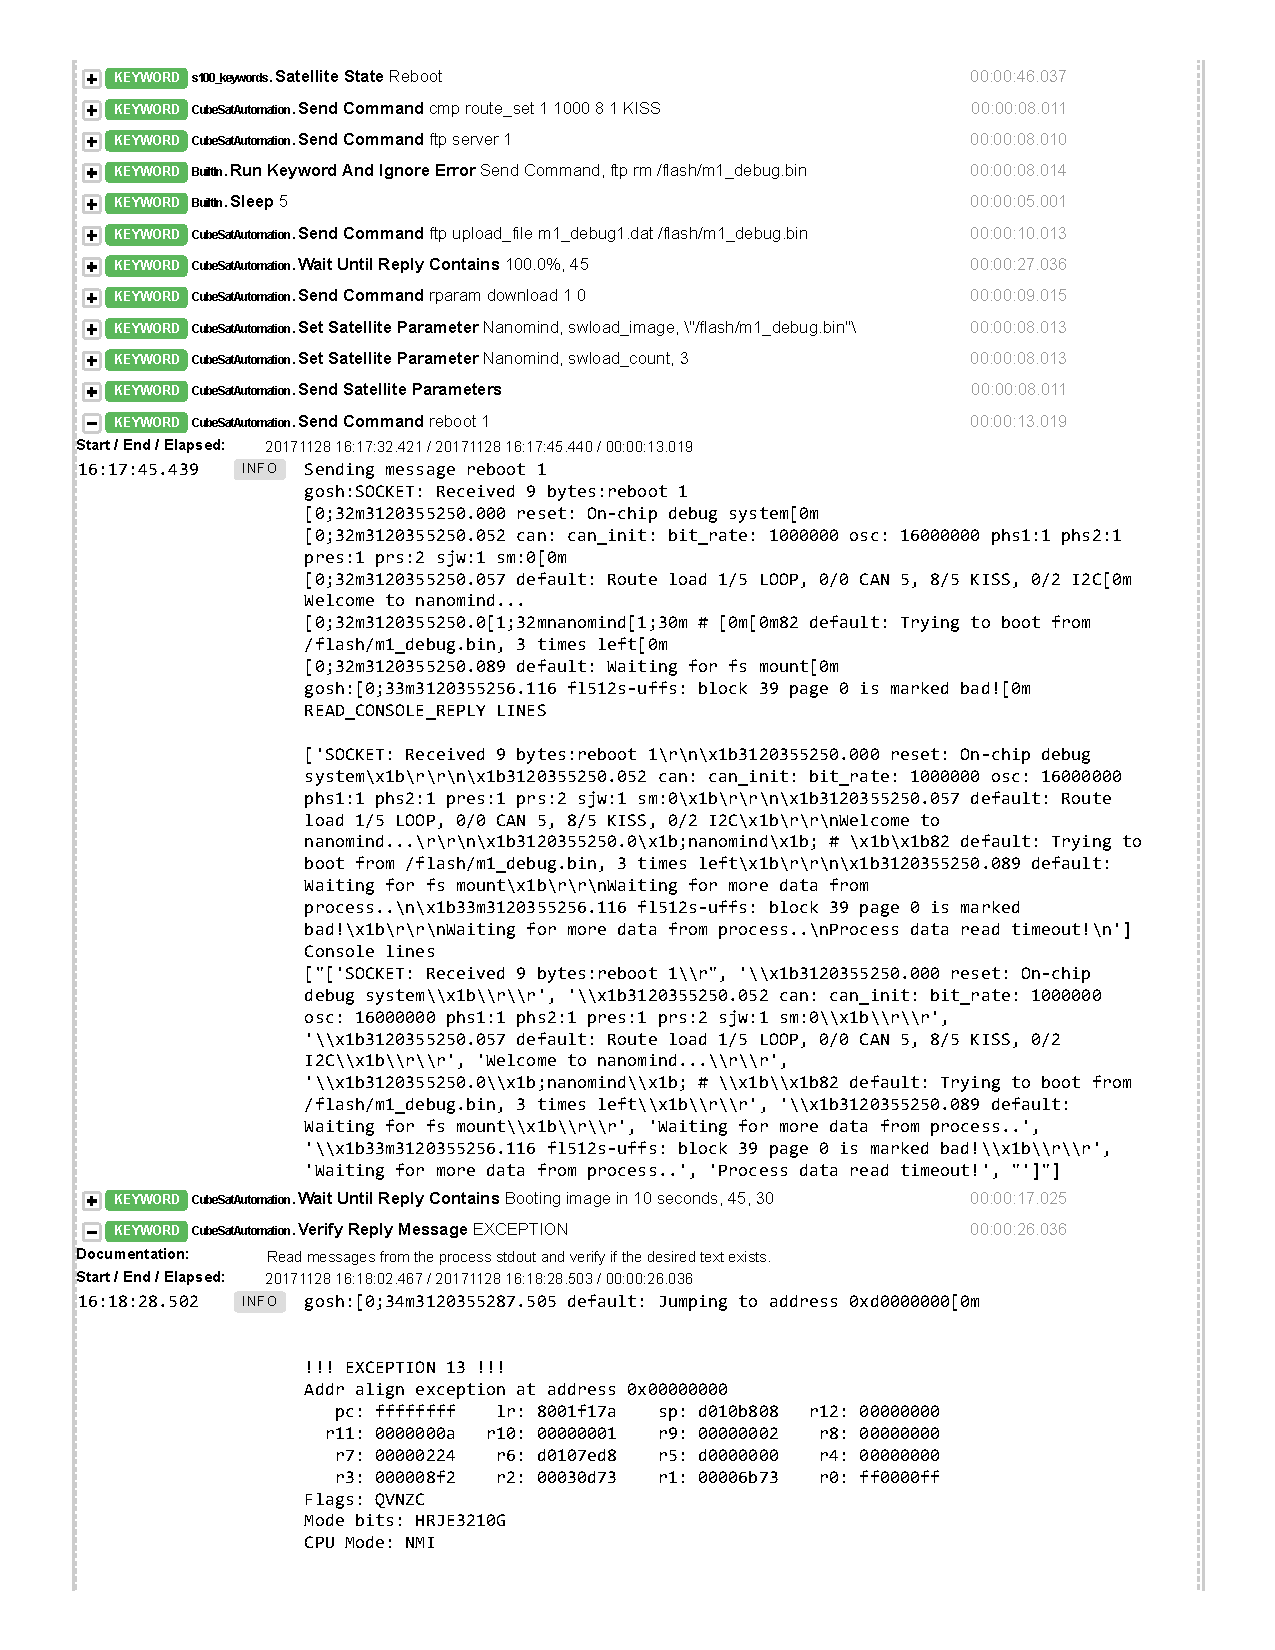
\includegraphics[scale=0.63]{result_pdf/example.pdf}\\
Figure D: Expanded Robot Framework test log file.
\label{logexample}
\end{center}
\begin{center}
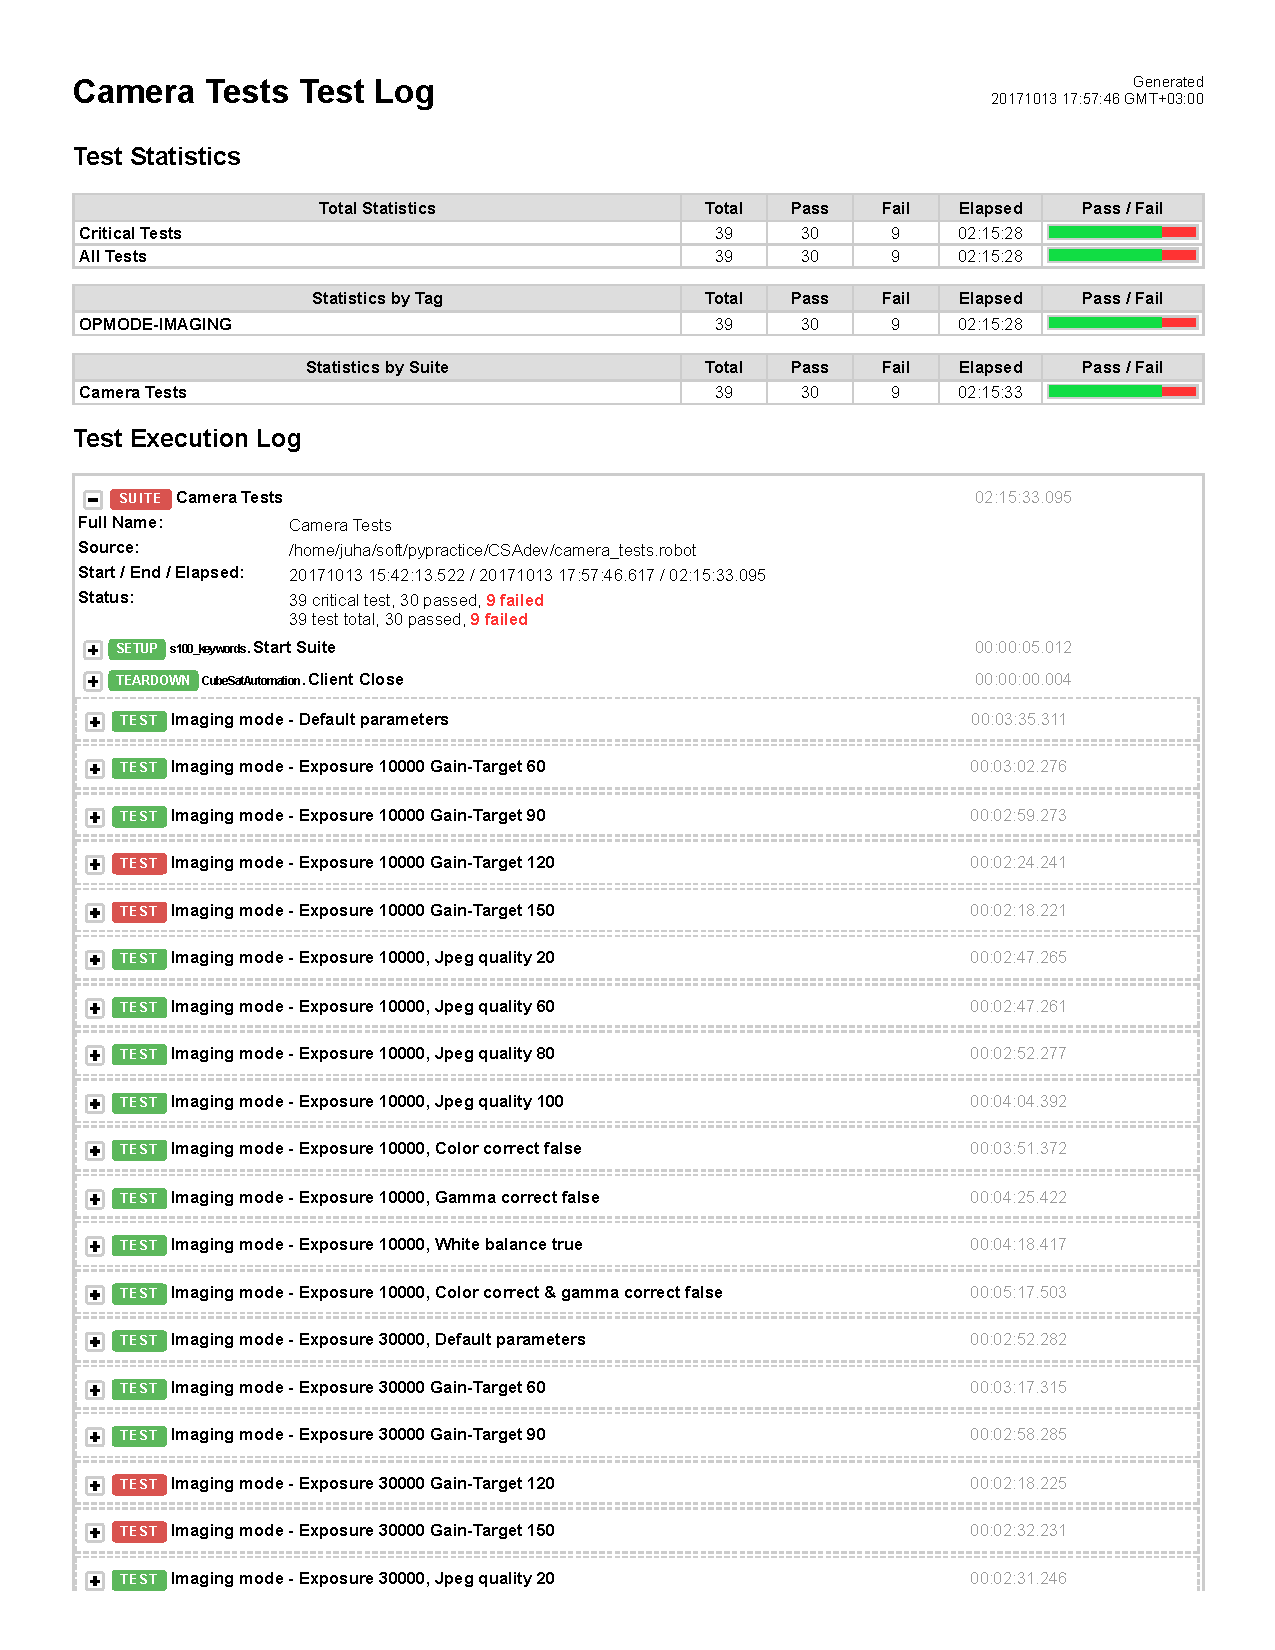
\includepdf[pages=1-2, pagecommand={}, width=\textwidth, offset=73pt 0pt]{result_pdf/Camera_Tests_Test_Log.pdf}
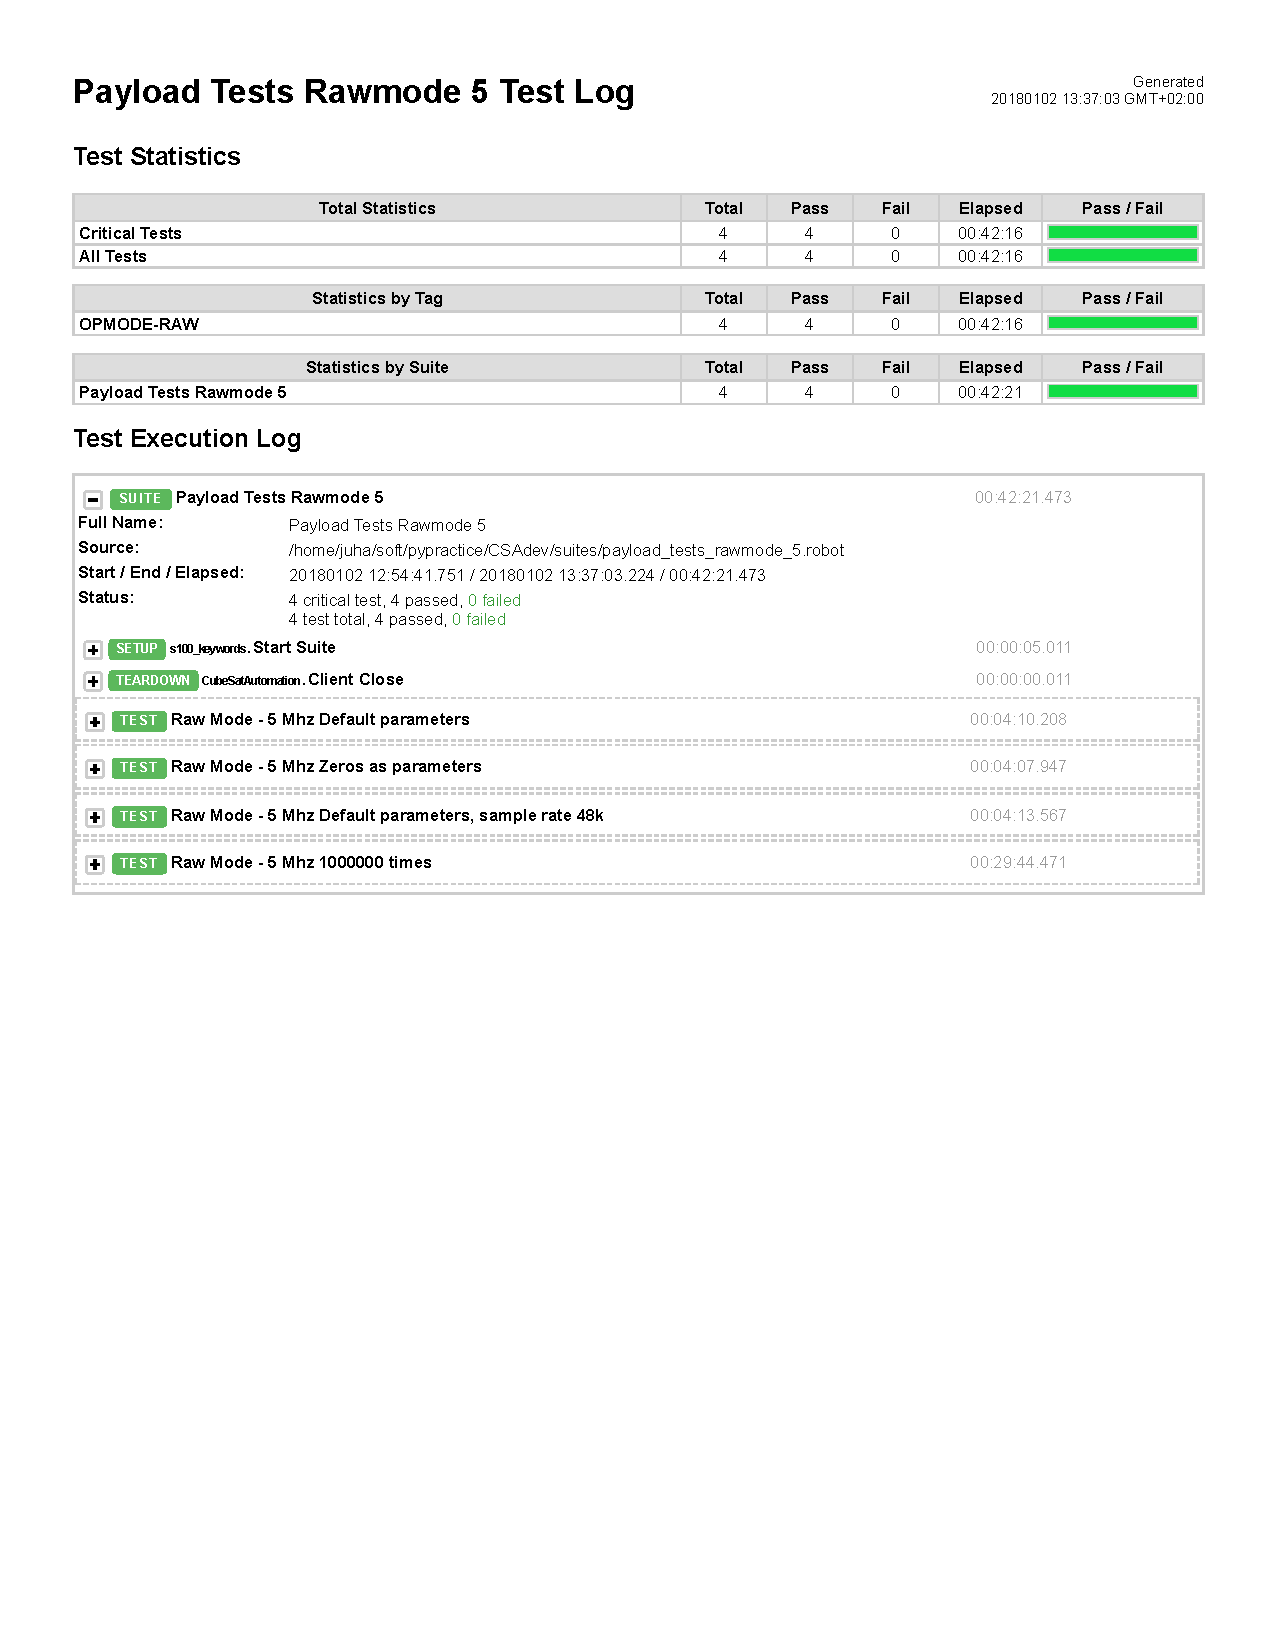
\includepdf[pagecommand={}, width=\textwidth, offset=73pt 0pt]{result_pdf/Payload_Tests_Rawmode_5_Test_Log.pdf}
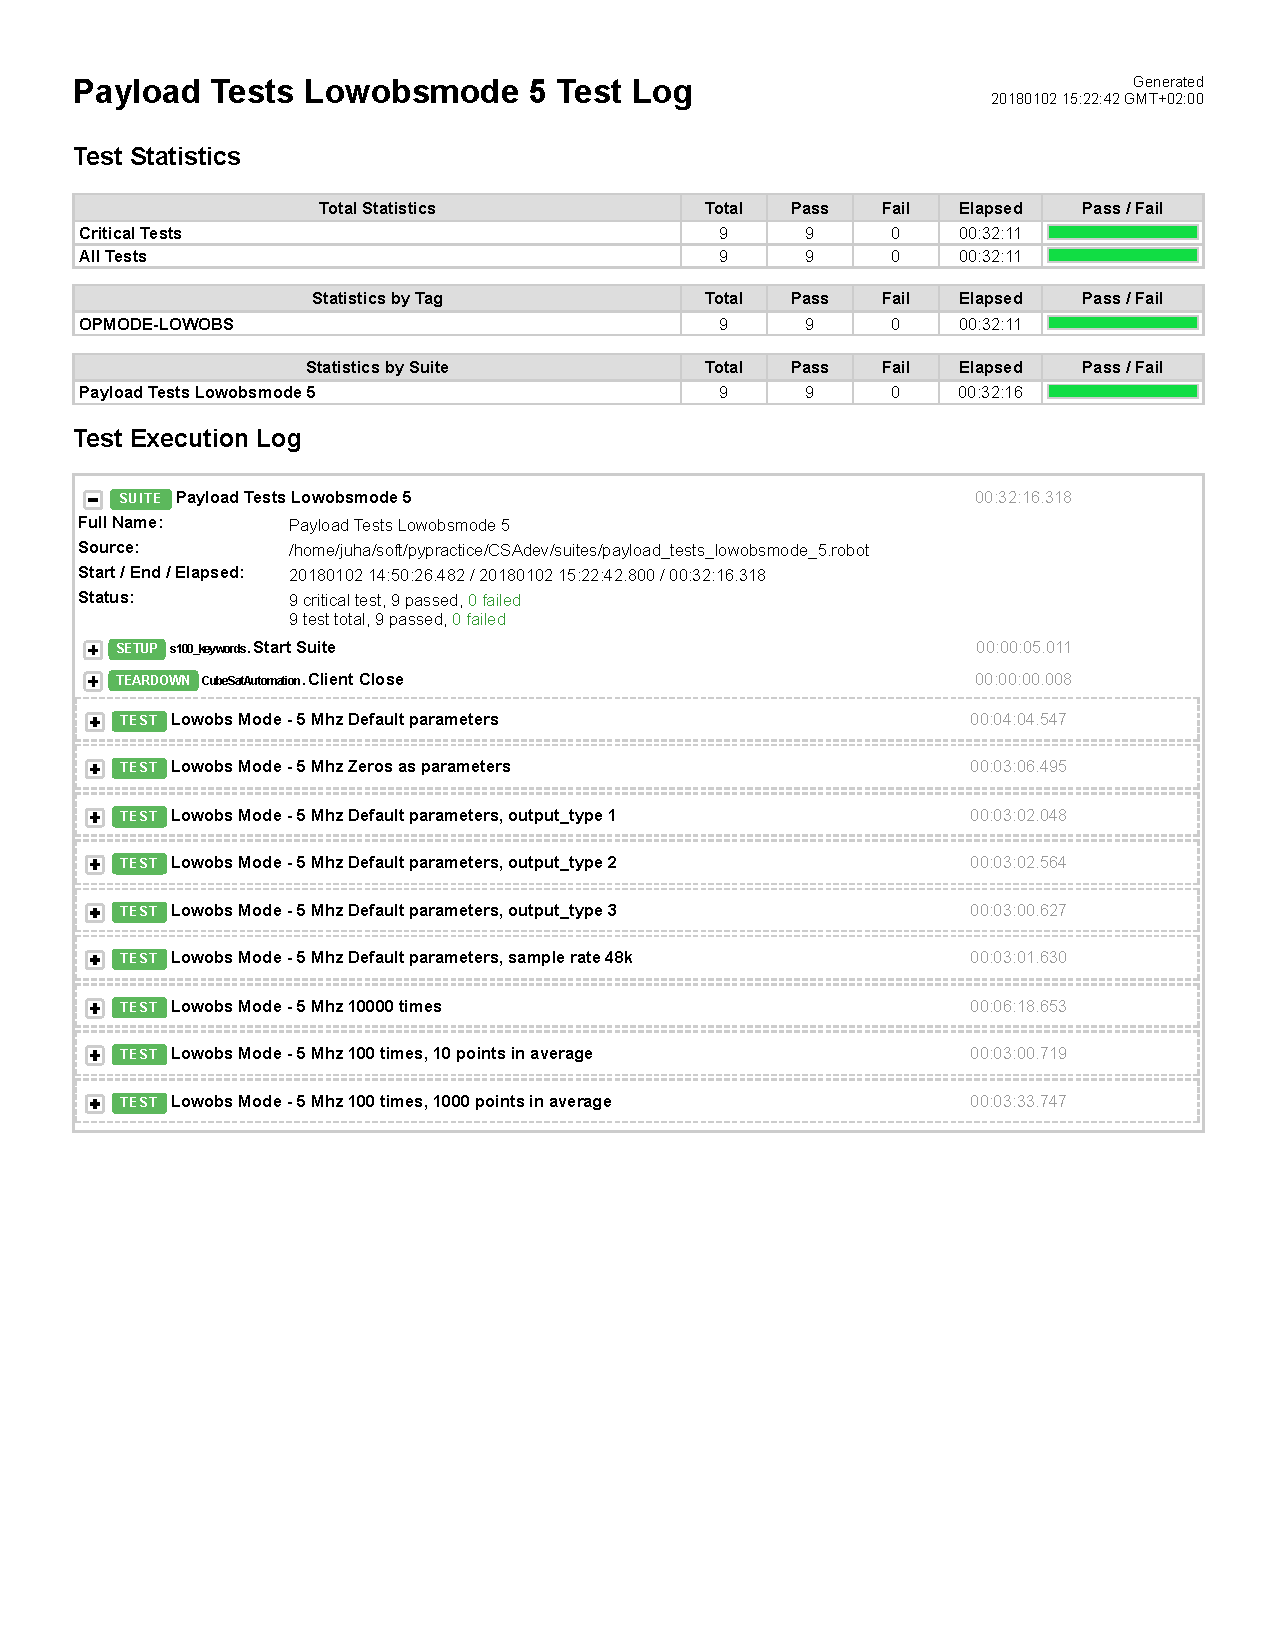
\includepdf[pagecommand={}, width=\textwidth, offset=73pt 0pt]{result_pdf/Payload_Tests_Lowobsmode_5_Test_Log.pdf}
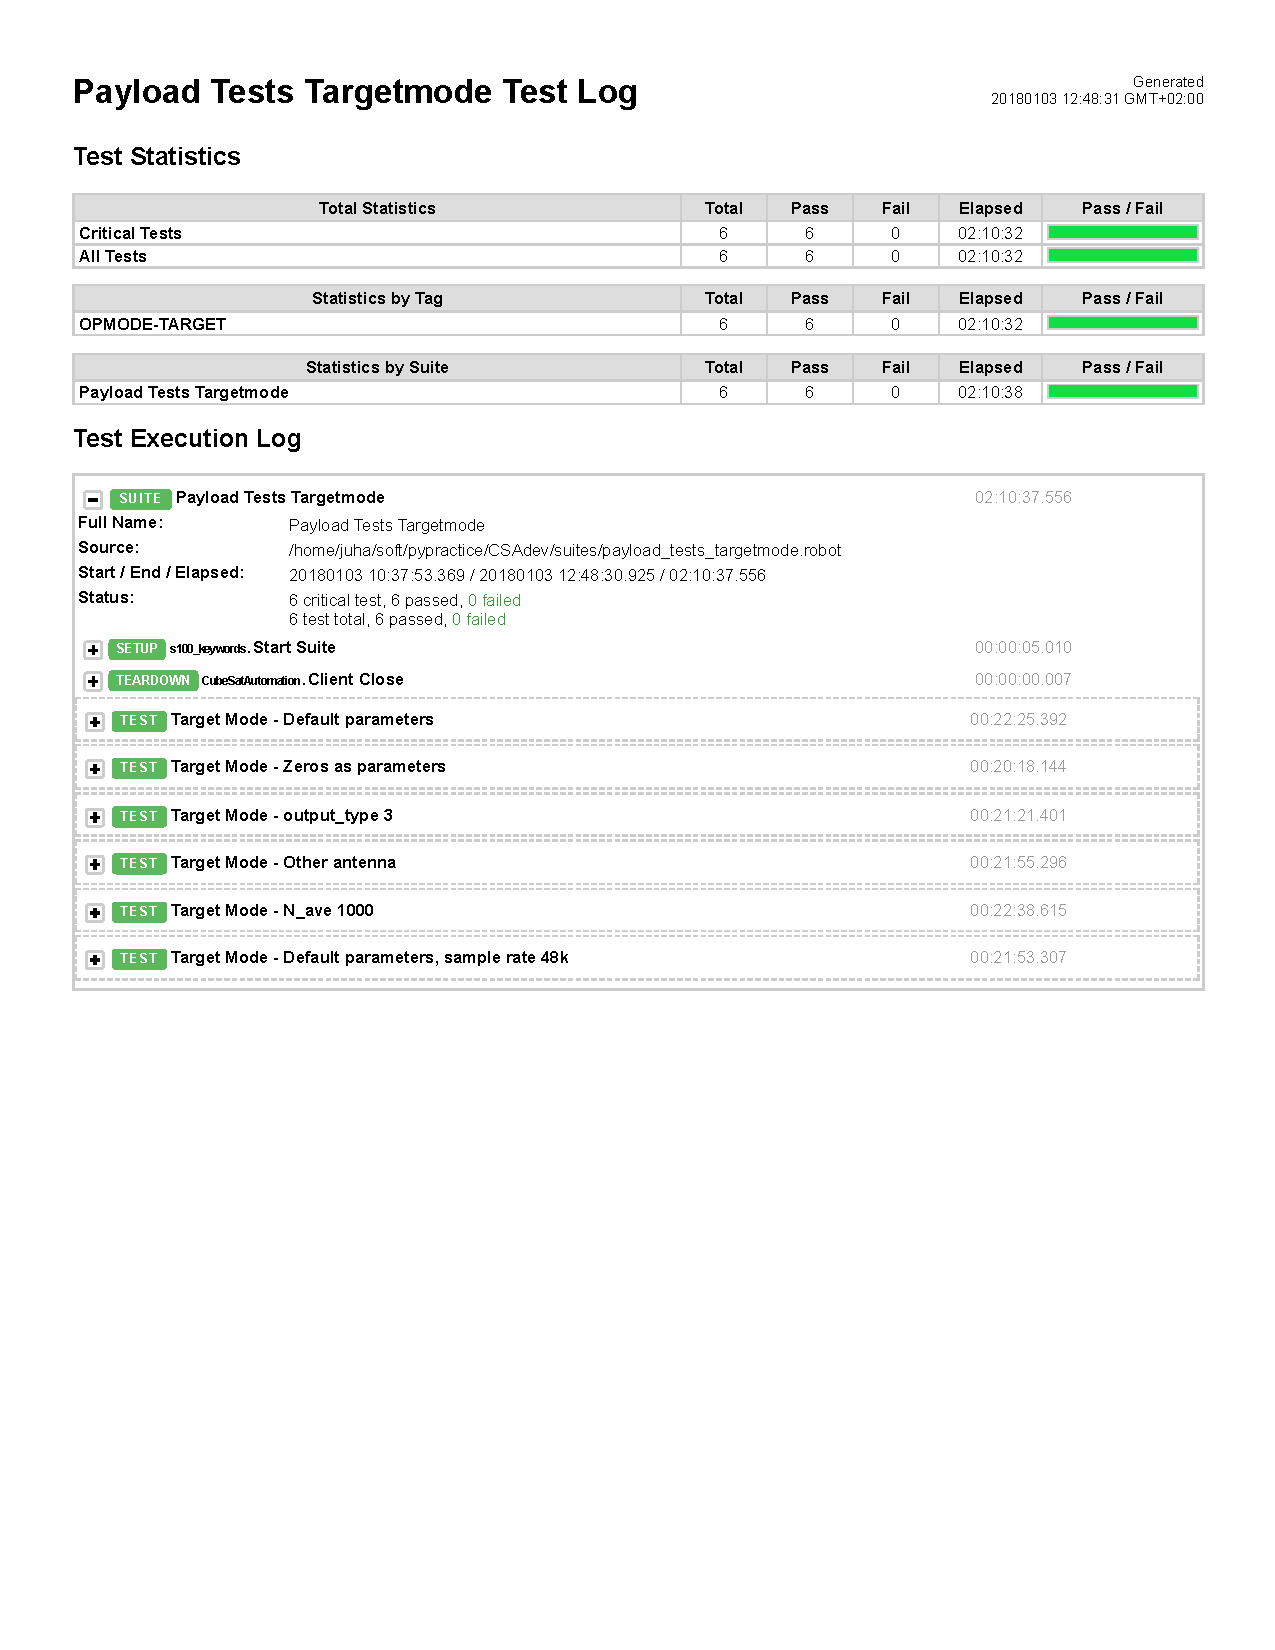
\includepdf[pagecommand={}, width=\textwidth, offset=73pt 0pt]{result_pdf/Payload_Tests_Targetmode_Test_Log.pdf}
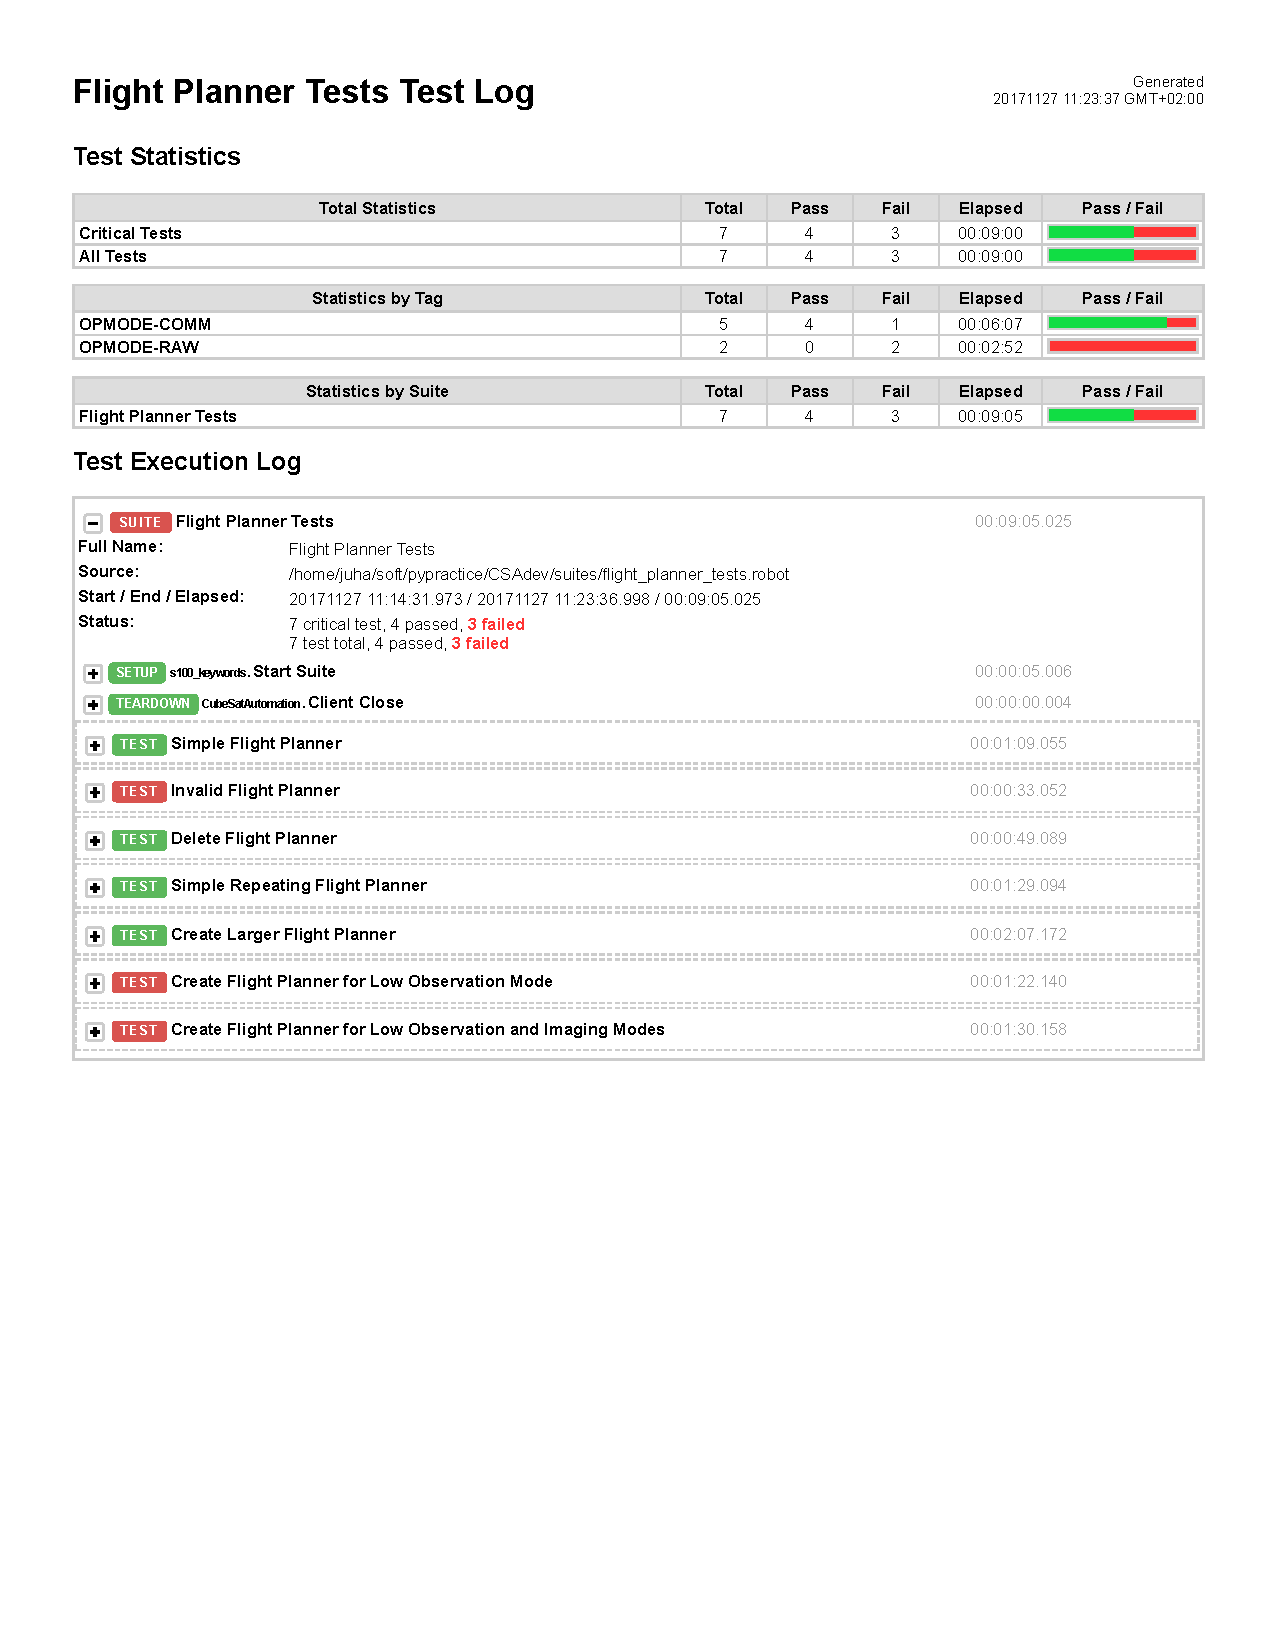
\includepdf[pagecommand={}, width=\textwidth, offset=73pt 0pt]{result_pdf/Flight_Planner_Tests_Test_Log.pdf}
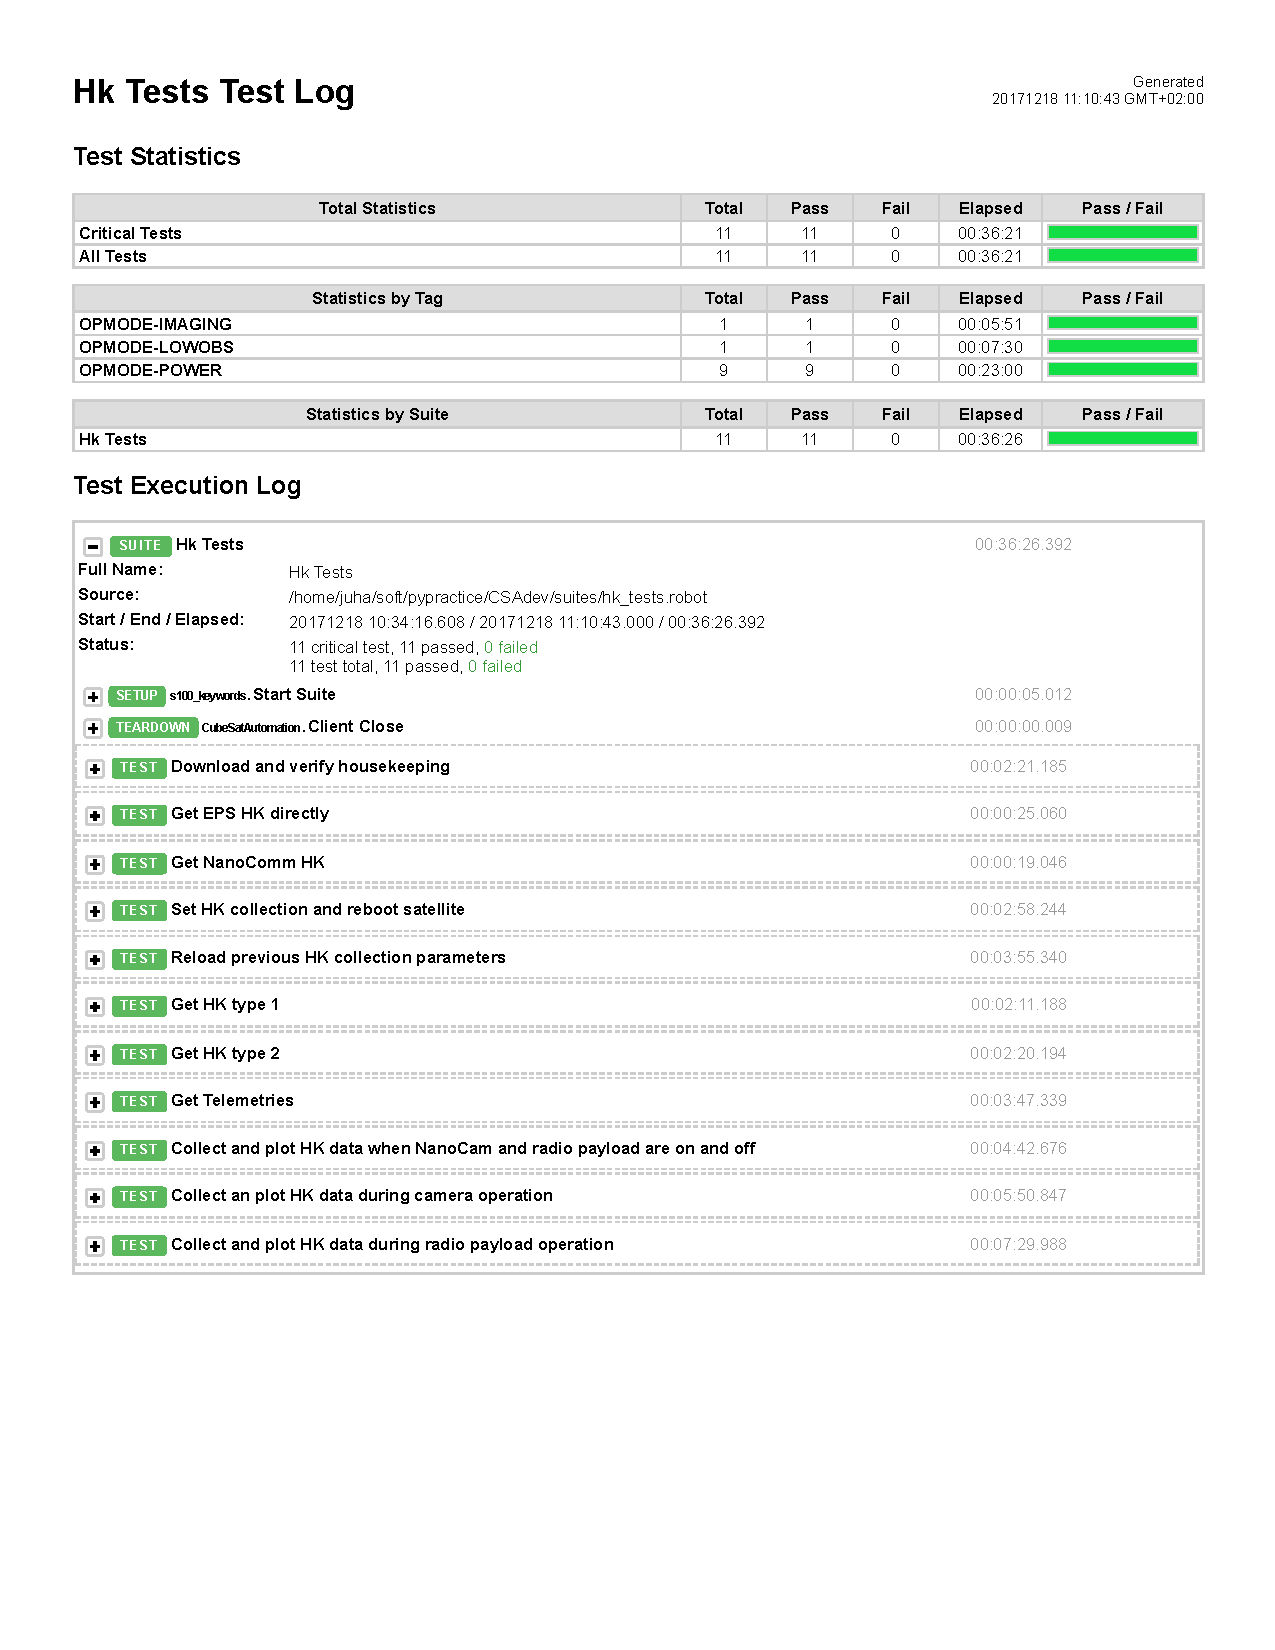
\includepdf[pagecommand={}, width=\textwidth, offset=73pt 0pt]{result_pdf/Hk_Tests_Test_Log.pdf}
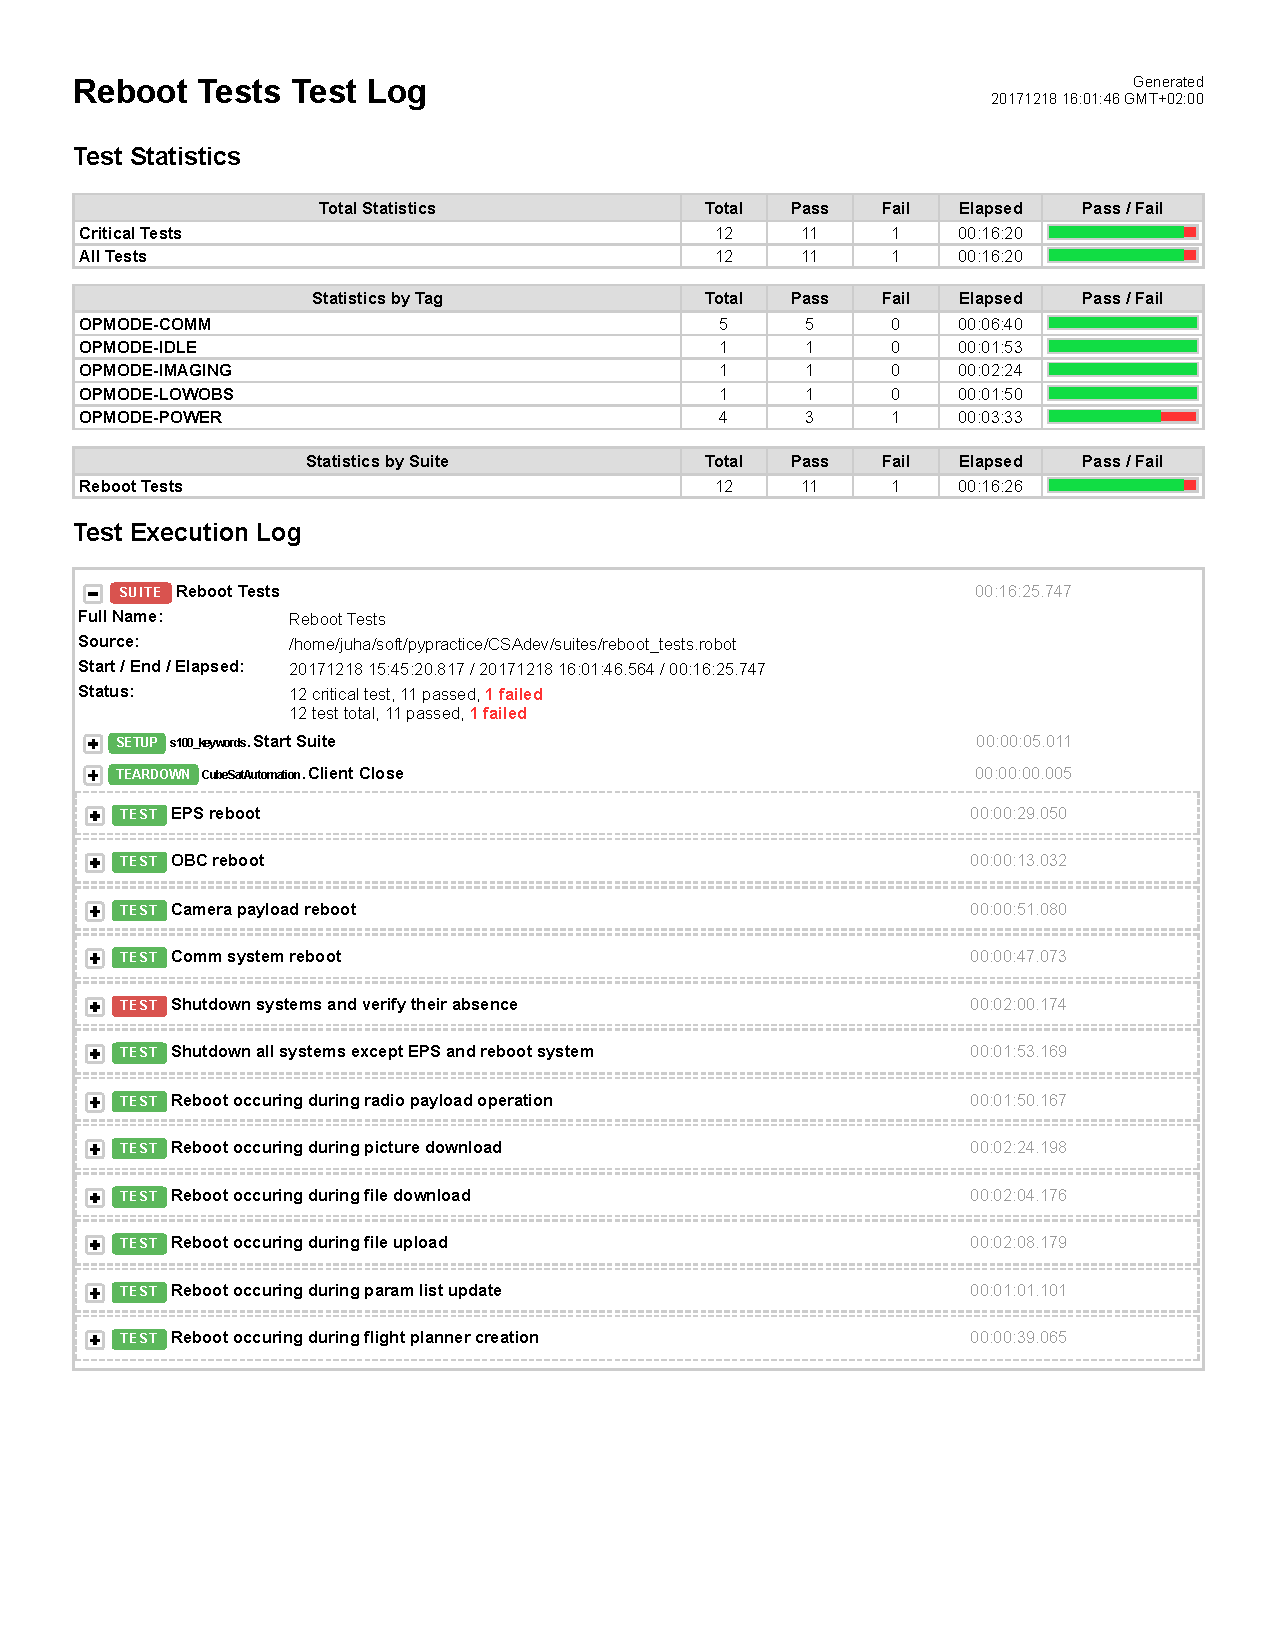
\includepdf[pagecommand={}, width=\textwidth, offset=73pt 0pt]{result_pdf/Reboot_Tests_Test_Log.pdf}
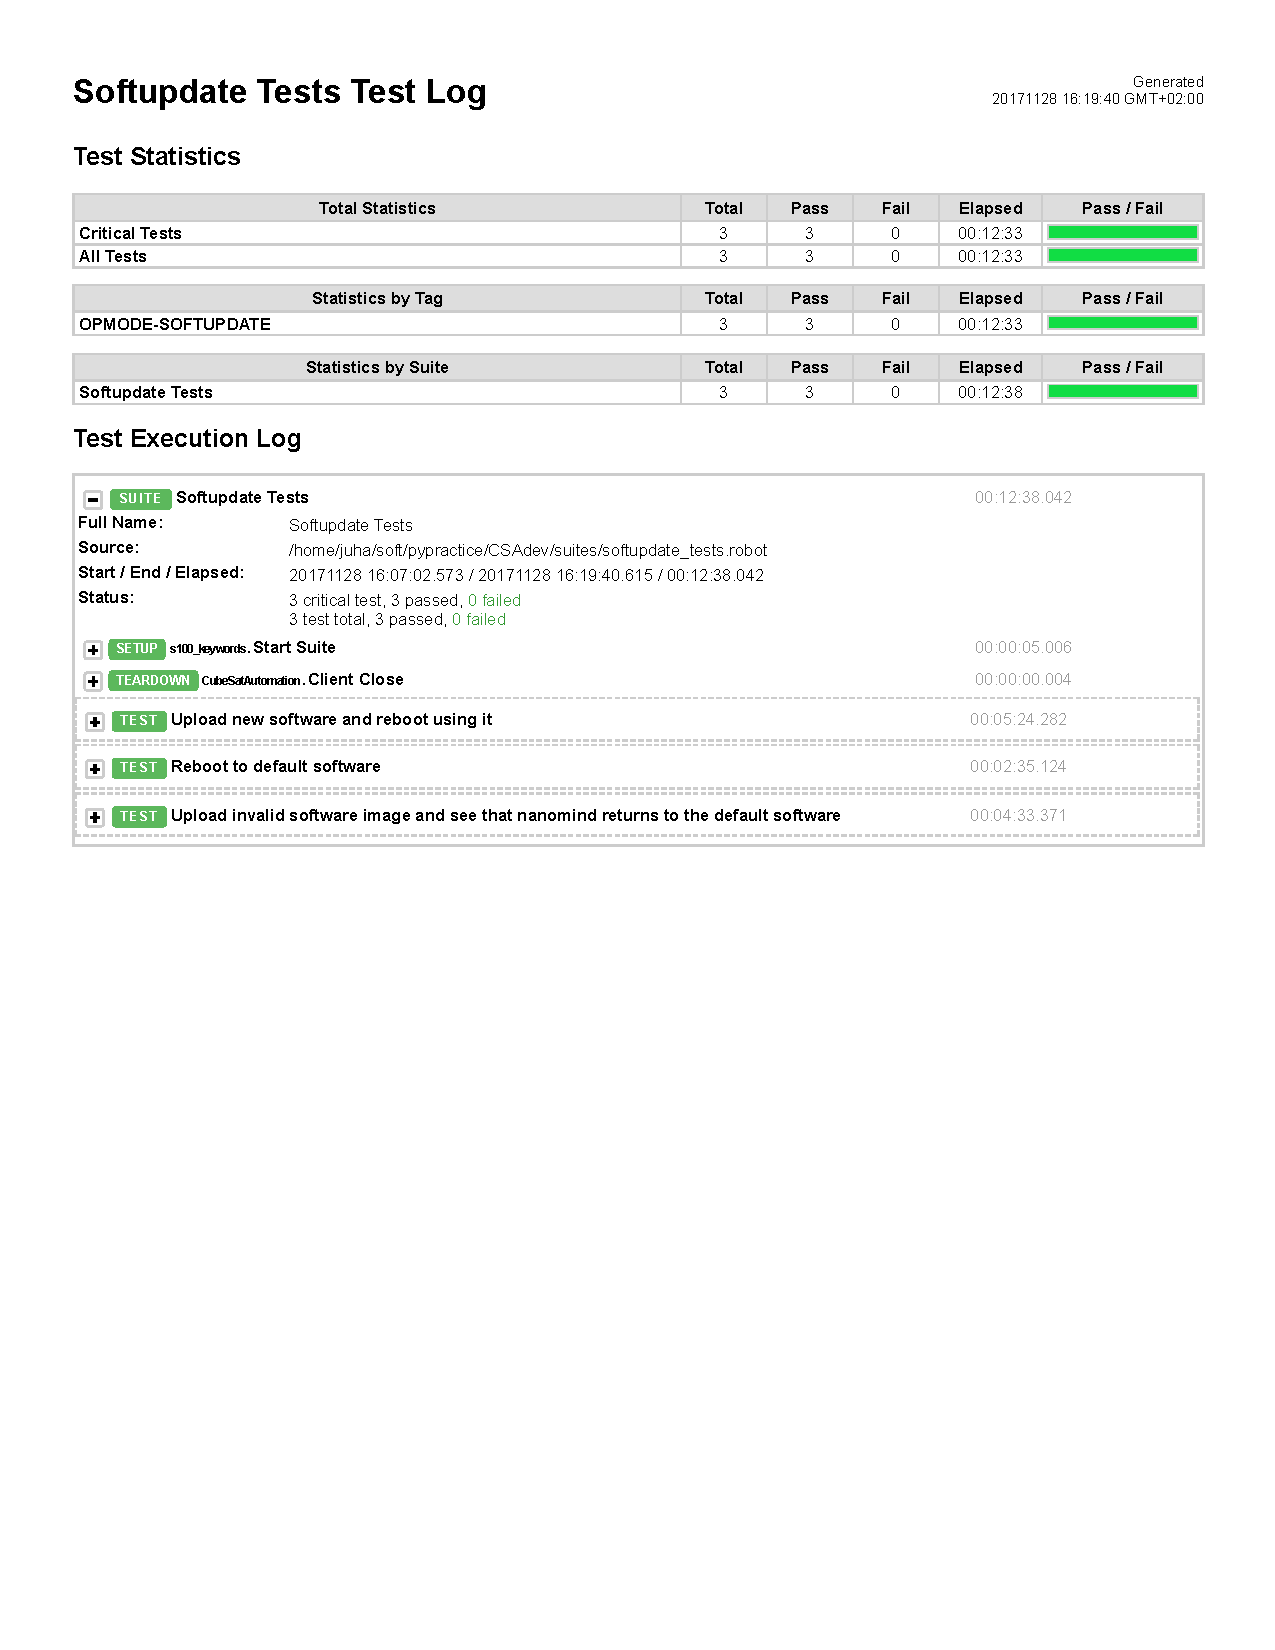
\includepdf[pagecommand={}, width=\textwidth, offset=73pt 0pt]{result_pdf/Softupdate_Tests_Test_Log.pdf}
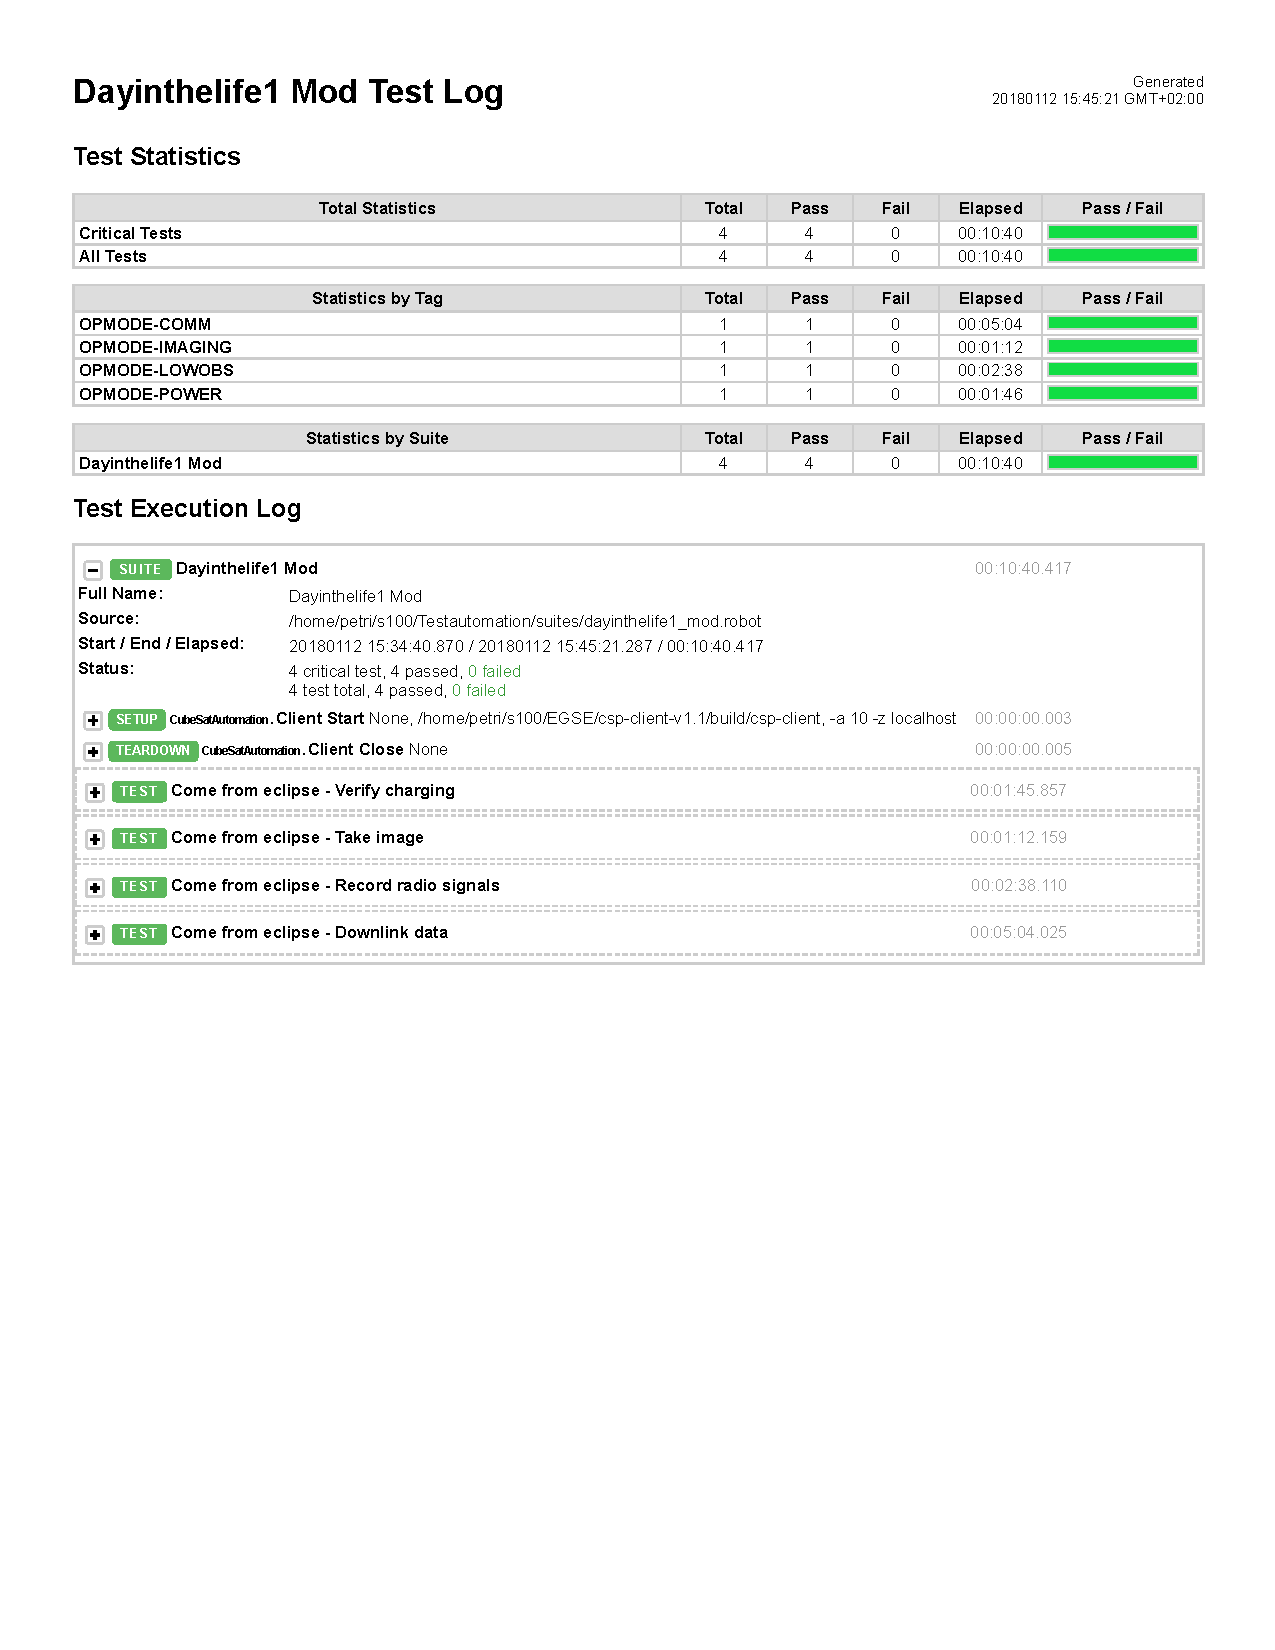
\includepdf[pagecommand={}, width=\textwidth, offset=73pt 0pt]{result_pdf/Dayinthelife1_Mod_Test_Log.pdf}
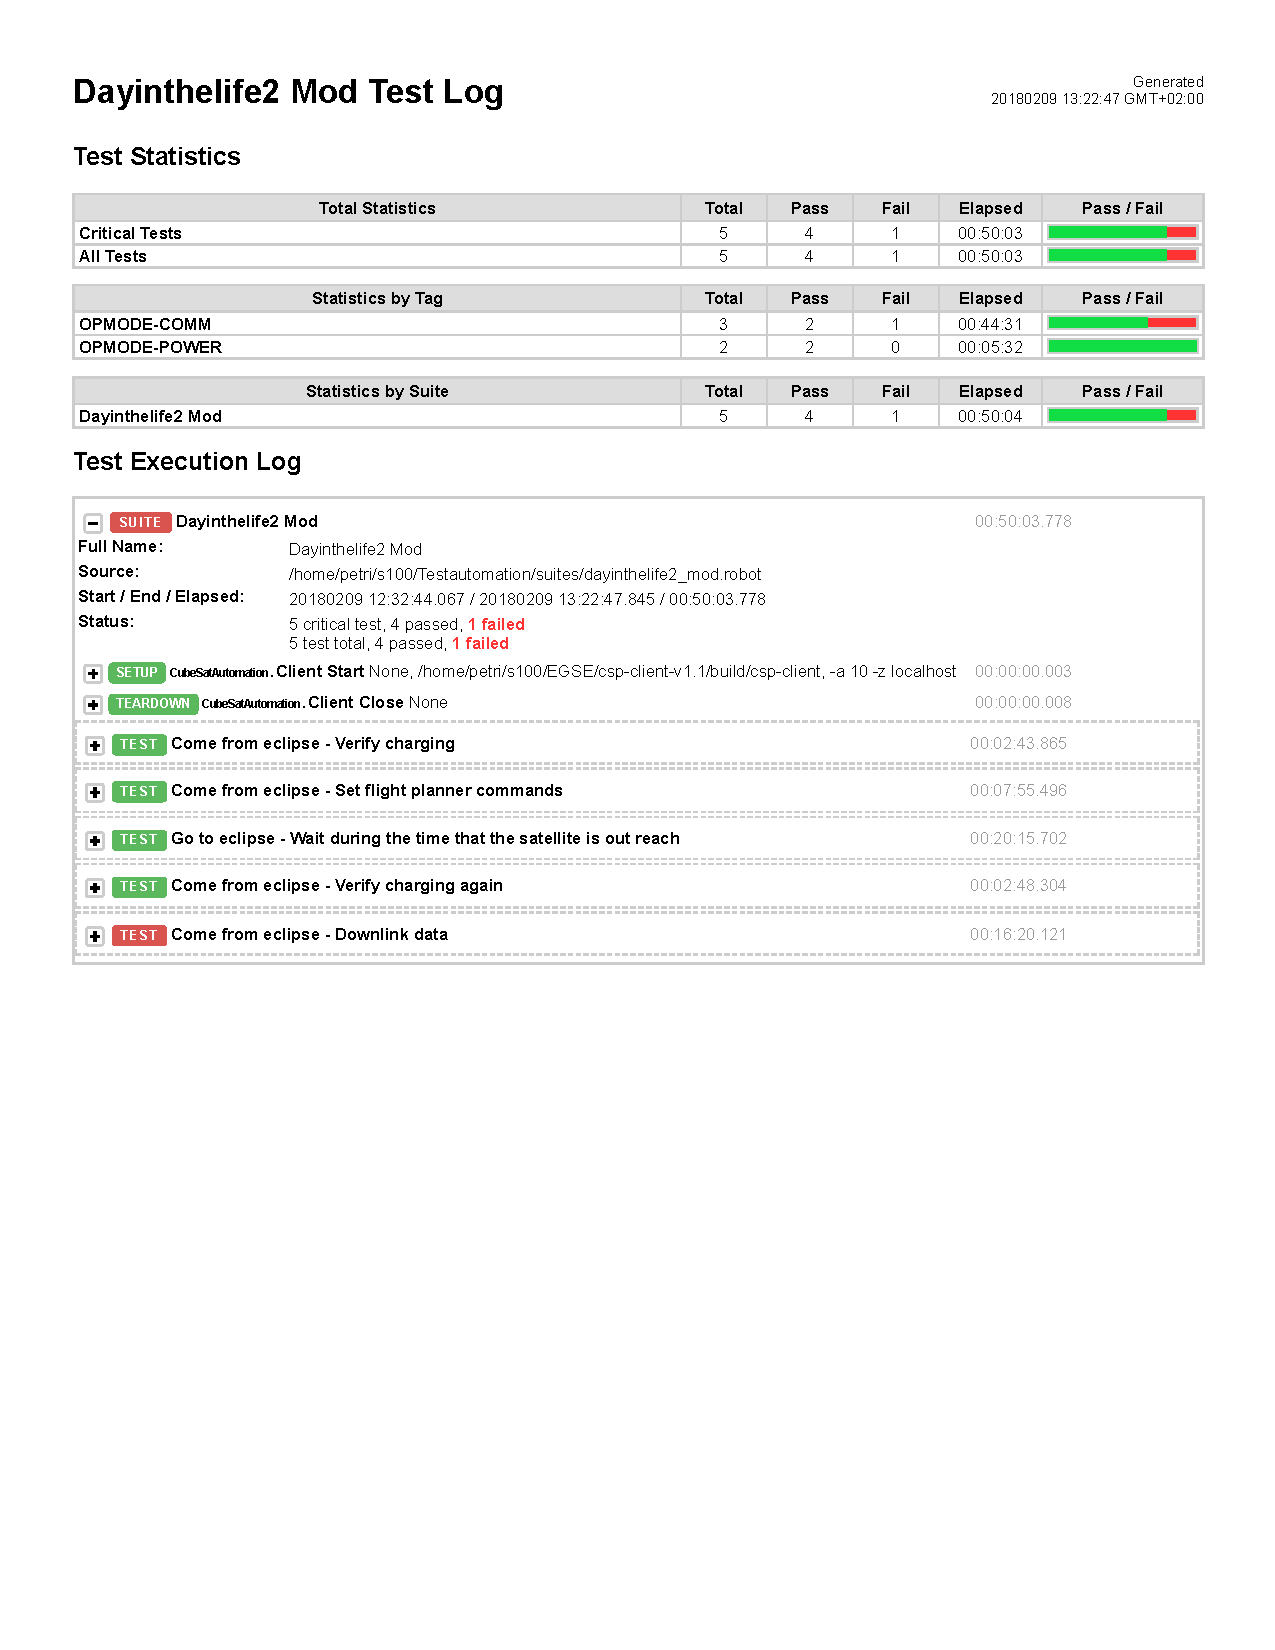
\includepdf[pagecommand={}, width=\textwidth, offset=73pt 0pt]{result_pdf/Dayinthelife2_Mod_Test_Log.pdf}
%\includepdf[pagecommand={}, width=\textwidth, offset=73pt 0pt]{result_pdf/%Dayinthelife3_Test_Log.pdf}
%\includepdf[pagecommand={}, width=\textwidth, offset=73pt 0pt]{result_pdf/%Dayinthelife4_Test_Log.pdf}
\end{center} 

\end{document}
